\documentclass[11pt]{article}

\usepackage[T1]{fontenc}
\usepackage[utf8]{inputenc}
\IfFileExists{libertinus.sty}{\usepackage{libertinus}}{\usepackage{lmodern}}
\usepackage{microtype}
\usepackage[a4paper,margin=27mm,headheight=15pt]{geometry}
\usepackage{amsmath,amssymb,amsthm,mathtools}
\usepackage{booktabs,longtable,array,tabularx}
\usepackage{graphicx}
\usepackage{float}
\usepackage{caption}
\usepackage{enumitem}
\usepackage{xcolor}
\usepackage{listings}
\usepackage{xurl}
\usepackage{hyperref}
\usepackage[nameinlink,noabbrev,capitalise]{cleveref}
\usepackage{aliascnt}

% Canonical project-wide mathematical notation.
% Canonical mathematical notation for active FabiusFunction LaTeX documents.
%
% This file is intentionally a plain TeX input rather than a LaTeX package.
% Every standalone document loads it by an explicit path relative to that
% document's directory; included fragments inherit the definitions from their
% root document.  Keep this file independent of document layout and metadata.
%
% Contract:
%   * one command has one mathematical meaning throughout the active corpus;
%   * names encode semantic roles rather than a document-local choice of letter;
%   * visually similar but differently normalized objects have different print;
%   * every command below is defined normatively in the notation catalogue.
%
% The active corpus excludes docs/archive/.  Historical sources may retain
% their original notation only inside an explicitly labelled quotation.

\makeatletter
\@ifundefined{mathbb}{%
  \PackageError{fabius-notation}{The amssymb package must be loaded first}%
    {Load amsmath and amssymb before inputting fabius-notation.tex.}%
}{}
\@ifundefined{operatorname}{%
  \PackageError{fabius-notation}{The amsmath package must be loaded first}%
    {Load amsmath before inputting fabius-notation.tex.}%
}{}
\makeatother

% Version stamp used by the catalogue and by static audits.
\newcommand{\FabiusNotationVersion}{2026-08-31}

% Number systems.  NaturalNumbers is explicitly the nonnegative convention.
\newcommand{\NaturalNumbers}{\mathbb{N}_{0}}
\newcommand{\PositiveIntegers}{\mathbb{N}_{>0}}
\newcommand{\IntegerNumbers}{\mathbb{Z}}
\newcommand{\RationalNumbers}{\mathbb{Q}}
\newcommand{\RealNumbers}{\mathbb{R}}
\newcommand{\ComplexNumbers}{\mathbb{C}}
\newcommand{\ExtendedRealNumbers}{\overline{\mathbb{R}}}

% The three principal Fabius--Rvachev functions.  Subscripts are deliberate:
% a bare F and a calligraphic F have several unrelated uses in the corpus.
\newcommand{\FabiusBounded}{F_{\mathrm{bd}}}
\newcommand{\FabiusGlobal}{F_{\mathrm{gl}}}
\newcommand{\FabiusQuantile}{Q_{F}}
\newcommand{\FabiusClampedQuantile}{Q_{F,\mathrm{cl}}}
\newcommand{\RvachevUp}{\operatorname{up}}

% Constants, elementary operators, and delimiters.
\newcommand{\EulerE}{\mathrm{e}}
\newcommand{\ImaginaryUnit}{\mathrm{i}}
\newcommand{\Differential}{\mathop{}\!\mathrm{d}}
\newcommand{\AbsoluteValue}[1]{\left\lvert #1\right\rvert}
\newcommand{\Norm}[1]{\left\lVert #1\right\rVert}
\newcommand{\Floor}[1]{\left\lfloor #1\right\rfloor}
\newcommand{\Ceiling}[1]{\left\lceil #1\right\rceil}
\newcommand{\FractionalPart}[1]{\left\{#1\right\}}
\newcommand{\PositivePart}[1]{\left(#1\right)_{+}}
\newcommand{\IndicatorOf}[1]{\mathbf{1}_{#1}}
\newcommand{\SetOf}[1]{\left\{#1\right\}}
\newcommand{\InnerProduct}[1]{\left\langle #1\right\rangle}
\newcommand{\CardinalityOf}[1]{\left\lvert #1\right\rvert}
\newcommand{\DefinitionEquals}{\mathrel{\coloneqq}}
\newcommand{\Sign}{\operatorname{sgn}}
\newcommand{\IdentityOperator}{\operatorname{id}}
\newcommand{\SpanOperator}{\operatorname{span}}
\newcommand{\TraceOperator}{\operatorname{tr}}
\newcommand{\RankOperator}{\operatorname{rank}}
\newcommand{\DiagonalOperator}{\operatorname{diag}}
\newcommand{\ResidueOperator}{\operatorname*{Res}}
\newcommand{\LeastCommonMultiple}{\operatorname{lcm}}
\newcommand{\OrderOperator}{\operatorname{ord}}
\newcommand{\PrincipalLogarithm}{\operatorname{Log}}
\newcommand{\FallingFactorial}[2]{\left(#1\right)^{\underline{#2}}}
\newcommand{\RisingFactorial}[2]{\left(#1\right)^{\overline{#2}}}

% Support, topology, convolution, and metric notation.
\newcommand{\SupportOperator}{\operatorname{supp}}
\newcommand{\SupportOf}[1]{\SupportOperator\!\left(#1\right)}
\newcommand{\TopologicalSupportOf}[1]{\operatorname{tsupp}\!\left(#1\right)}
\newcommand{\Convolution}{\mathbin{*}}
\newcommand{\MetricDistance}{\operatorname{dist}}
\newcommand{\TotalVariationDistance}{d_{\mathrm{TV}}}

% Probability.  Equality and convergence in law are not metric distance.
\newcommand{\Probability}{\mathbb{P}}
\newcommand{\Expectation}{\mathbb{E}}
\newcommand{\Variance}{\operatorname{Var}}
\newcommand{\Covariance}{\operatorname{Cov}}
\newcommand{\LawOperator}{\operatorname{Law}}
\newcommand{\LawOf}[1]{\LawOperator\!\left(#1\right)}
\newcommand{\EqualInLaw}{\mathrel{\overset{\mathrm{law}}{=}}}
\newcommand{\ConvergesInLaw}{\mathrel{\xrightarrow{\mathrm{law}}}}

% Fourier and integral transforms.  The printed labels expose normalization.
% FourierTwoPi uses exp(-2*pi*i*x*xi); FourierAngular uses exp(-i*x*omega).
\newcommand{\FourierTwoPi}[1]{\widehat{#1}_{\,2\pi}}
\newcommand{\FourierAngular}[1]{\widehat{#1}_{\,\mathrm{ang}}}
\newcommand{\LaplaceTransformSymbol}{\mathcal{L}}
\newcommand{\MellinTransformSymbol}{\mathcal{M}}
\newcommand{\LaplaceTransformOf}[1]{\LaplaceTransformSymbol\!\left[#1\right]}
\newcommand{\MellinTransformOf}[1]{\MellinTransformSymbol\!\left[#1\right]}
\newcommand{\MomentGeneratingFunction}[1]{M_{#1}}
\newcommand{\CharacteristicFunction}[1]{\varphi_{#1}}

% The two standard sinc functions must never share one symbol.
\newcommand{\SincRad}{\operatorname{sinc}_{\mathrm{rad}}}
\newcommand{\SincPi}{\operatorname{sinc}_{\pi}}

% Binary arithmetic and Thue--Morse notation.
\newcommand{\BinaryDigitSum}{\operatorname{wt}_{2}}
\newcommand{\ThueMorseSignSymbol}{\varepsilon}
\newcommand{\ThueMorseSign}[1]{\varepsilon_{#1}}
\newcommand{\PadicValuation}[1]{\nu_{#1}}
\newcommand{\TwoAdicValuation}{\nu_{2}}

% q-series notation.  Every base is an explicit argument.
\newcommand{\QPochhammer}[3]{\left(#1;#2\right)_{#3}}
\newcommand{\GaussianBinomial}[3]{%
  \genfrac{[}{]}{0pt}{}{#1}{#2}_{#3}%
}
\newcommand{\QInteger}[2]{\left[#1\right]_{#2}}

% Named special functions.
\newcommand{\Polylogarithm}{\operatorname{Li}}
\newcommand{\LambertW}{W}
\newcommand{\GammaFunction}{\Gamma}
\newcommand{\RiemannZeta}{\zeta}

% Asymptotics.  BigO and LittleO are operator tokens for existing formula
% grammar; prefer the At forms so that the limiting regime is printed.
\newcommand{\BigO}{\mathcal{O}}
\newcommand{\LittleO}{o}
\newcommand{\BigOAt}[2]{\mathcal{O}_{#2}\!\left(#1\right)}
\newcommand{\LittleOAt}[2]{o_{#2}\!\left(#1\right)}


\graphicspath{{figures/}}
\allowdisplaybreaks
\setcounter{tocdepth}{2}
\setcounter{secnumdepth}{3}
\setlist{nosep}
\hypersetup{
  colorlinks=true,
  linkcolor=blue!55!black,
  citecolor=green!35!black,
  urlcolor=blue!55!black,
  pdftitle={The Lambert W Function: A Real-Variable Guide with Proofs},
  pdfauthor={},
  pdfsubject={Lambert W function, real branches, asymptotics, approximations, numerical methods}
}

% ed.: these share the `theorem' counter for a single numbering sequence, but
% ed.: declared as \newtheorem{X}[theorem]{...} they also report that counter
% ed.: name to cleveref, so every \Cref to a lemma, proposition, corollary,
% ed.: definition, example, algorithm, remark, literature note or branch
% ed.: warning printed ``Theorem''.  aliascnt keeps the shared numbering and
% ed.: restores the true type.
\newtheorem{theorem}{Theorem}[section]

\newaliascnt{lemma}{theorem}
\newtheorem{lemma}[lemma]{Lemma}
\aliascntresetthe{lemma}

\newaliascnt{proposition}{theorem}
\newtheorem{proposition}[proposition]{Proposition}
\aliascntresetthe{proposition}

\newaliascnt{corollary}{theorem}
\newtheorem{corollary}[corollary]{Corollary}
\aliascntresetthe{corollary}

\newaliascnt{definition}{theorem}
\newtheorem{definition}[definition]{Definition}
\aliascntresetthe{definition}

\newaliascnt{example}{theorem}
\newtheorem{example}[example]{Example}
\aliascntresetthe{example}

\newaliascnt{algorithm}{theorem}
\newtheorem{algorithm}[algorithm]{Algorithm}
\aliascntresetthe{algorithm}

\theoremstyle{remark}
\newaliascnt{remark}{theorem}
\newtheorem{remark}[remark]{Remark}
\aliascntresetthe{remark}

\newaliascnt{literaturenote}{theorem}
\newtheorem{literaturenote}[literaturenote]{Literature note}
\aliascntresetthe{literaturenote}

\newaliascnt{warning}{theorem}
\newtheorem{warning}[warning]{Branch warning}
\aliascntresetthe{warning}

\crefname{lemma}{lemma}{lemmas}
\Crefname{lemma}{Lemma}{Lemmas}
\crefname{proposition}{proposition}{propositions}
\Crefname{proposition}{Proposition}{Propositions}
\crefname{corollary}{corollary}{corollaries}
\Crefname{corollary}{Corollary}{Corollaries}
\crefname{definition}{definition}{definitions}
\Crefname{definition}{Definition}{Definitions}
\crefname{example}{example}{examples}
\Crefname{example}{Example}{Examples}
\crefname{algorithm}{algorithm}{algorithms}
\Crefname{algorithm}{Algorithm}{Algorithms}
\crefname{remark}{remark}{remarks}
\Crefname{remark}{Remark}{Remarks}
\crefname{literaturenote}{literature note}{literature notes}
\Crefname{literaturenote}{Literature note}{Literature notes}
\crefname{warning}{branch warning}{branch warnings}
\Crefname{warning}{Branch warning}{Branch warnings}

\newcommand{\Wz}{\LambertW_{0}}
\newcommand{\Wm}{\LambertW_{-1}}
% Crosswalk macros, as in the other frontier volumes: a Lean module or
% declaration name, typeset verbatim.
\newcommand{\lean}[1]{%
  \ifmmode\text{\texttt{\detokenize{#1}}}\else\nolinkurl{#1}\fi}
\newcommand{\leansubtwo}[2]{%
  \nolinkurl{#1}\texttt{\textsubscript{2}}\nolinkurl{#2}}
\newcommand{\decl}[1]{\nolinkurl{#1}}
\newcommand{\stirling}[2]{\genfrac{[}{]}{0pt}{}{#1}{#2}}
\newcommand{\brak}[1]{\left(#1\right)}
% LOCAL-NON-FOURIER-HAT: \LambertRootApproximation denotes a numerical approximation to the exact Lambert root on the selected real branch.
\newcommand{\LambertRootApproximation}{\widehat w}

\lstdefinestyle{pythonstyle}{
  language=Python,
  basicstyle=\ttfamily\small,
  breaklines=true,
  showstringspaces=false,
  frame=single,
  columns=fullflexible,
  keywordstyle=\bfseries,
  commentstyle=\itshape
}
\lstset{style=pythonstyle}

\title{\textbf{The Lambert \(W\) Function}\\
\large A Real-Variable Guide to Its Branches, Identities, Series,
Asymptotics, Bounds, Approximations, and Computation\\[0.5em]
\normalsize Consolidated edition merging four independent treatments}
\author{}
\date{Consolidated 28 August 2026}

\begin{document}
\maketitle

\begin{abstract}
The Lambert \(W\) function is the inverse of the elementary-looking map
\(w\mapsto w\EulerE^w\).  It is the natural language for equations in which an
unknown occurs both outside and inside an exponential.  This article develops
the function from first principles, at a level intended to be accessible after
a standard sophomore course in calculus and a first course in proof.  Special
attention is paid to the two real branches: the principal branch \(\Wz\) and
the nonprincipal branch \(\Wm\).  We prove their domains, ranges,
monotonicity, curvature, derivative formulas, integral identities, power
series, square-root expansions at the common branch point, complete
logarithmic asymptotic expansions, rigorous elementary bounds, and
branch-safe Newton iterations.  We also derive rational and continued
fraction approximations, contour and real integral representations, and
closed forms for representative transcendental equations.

The supplied source archive contains the foundational paper of Corless,
Gonnet, Hare, Jeffrey, and Knuth~\cite{corless1996}, the NIST Digital Library
of Mathematical Functions entry~\cite{dlmf}, papers on analytic approximations, continued fractions,
certified high-precision evaluation, bounds for \(\Wm\), Schroeder-type
series, and applications in circuits, biochemical kinetics, ecology, and
prime asymptotics.  Those sources inform the presentation and bibliography.
All principal results used in the exposition are proved here.  Results that
are mentioned only as historical or bibliographical context are explicitly
labelled as such.  A fully commented Python program supplied with the article
reproduces the numerical figures.

This consolidated edition merges three further independently written treatments of the same material: their shared core agreed with the text theorem for theorem and constant for constant, and their unique layers --- the complete power-tower convergence theorem, inverse-Taylor corrections, the branch-exchange involution, a transcendence theorem, a practitioner's toolkit, additional worked applications, and the \(r\)-Lambert outlook --- are preserved in a dedicated complements section, with a four-way concordance appendix and a note on the role of \(W_{-1}\) in the surrounding Fabius--Rvachev corpus.
\end{abstract}

\subsection*{Provenance}
This volume is the 2026-08-28 editorial consolidation of four independently
written treatments of the Lambert $W$ function that arrived together in the
corpus inbox.  The body of the volume is the most complete of the four; the
unique layers of the other three are merged in
\cref{sec:complements}, and the four-way agreement record is
\cref{app:concordance}.  The verification material of all four --- figures,
data, and deterministic scripts --- is preserved under \path{assets/}; the
absorbed source documents themselves are deleted once merged (git history is
the archive, pinned by the SHA-256 hashes below).
Each synchronized source checkpoint is validated by exactly three successful
serial halt-on-error passes and the repository's PDF gates.  Later source changes
do not inherit an earlier checkpoint's render validation.  Exact page-count,
byte-count, and SHA-256 receipts for validated source/PDF pairs are kept externally
in the repository documentation so that neither artifact embeds a self-invalidating
fingerprint. No
\nolinkurl{SHA256SUMS*} ledger exists or participates in validation.
\begin{itemize}
\item \path{Lambert_W_Function_Article/Lambert_W_Function_Article.tex} (the spine)\\
{\footnotesize SHA-256 \path{5bca61c4e906ca8a92f283bc92913355ccd4aee26d65112b41474fd16862c6ba}}
\item \path{Lambert-W-Article/lambert_w_monograph.tex} (the monograph treatment)\\
{\footnotesize SHA-256 \path{7459739452dd0c5cce41328f395d5826f0910f9f4d1ee055dfa56c18044c68b1}}
\item \path{Lambert_W_article/lambert_w_article.tex} (the third treatment)\\
{\footnotesize SHA-256 \path{44126ef919f4f29f8f28554fc2c7a8c177f74db01fea135c90188dce84eeabd6}}
\item \path{Lambert-W-Function-article-4/Lambert-W-Function.tex} (the fourth treatment)\\
{\footnotesize SHA-256 \path{4b732dbafdb9c4c48ed999a1cfe4b9b06fb39fd248bb8fa6aa4cf4d0365c8302}}
\end{itemize}

\tableofcontents
\clearpage

\section{Why a new function is needed}

Elementary algebra teaches us how to undo addition, multiplication, integer
powers, and exponentials.  Difficulty appears when the unknown occupies two
different roles at once.  For example,
\[
   y\EulerE^y=7,\qquad
   \EulerE^{3t}=5t+2,\qquad
   s+\log s=10
\]
cannot generally be solved by a finite combination of the usual elementary
functions.  The first equation is so basic that it is sensible to name its
inverse.

\begin{definition}[Lambert \(W\) function]
A value \(w\) of the Lambert \(W\) function at \(z\) is any solution of
\begin{equation}\label{eq:defining}
       w\EulerE^w=z.
\end{equation}
Thus
\[
       w=W(z)\quad\Longleftrightarrow\quad w\EulerE^w=z.
\]
Because the complex exponential is periodic and the map \(w\mapsto w\EulerE^w\)
is not one-to-one, \(W\) has branches.  The branches are denoted \(W_k\),
where \(k\in\IntegerNumbers\).  On the real line only \(W_0\) and \(W_{-1}\) can
take real values.
\end{definition}

The symbol \(W\) is not an unexplained trick: it records an inverse operation,
just as \(\sqrt{\phantom{x}}\), \(\log\), and \(\arcsin\) do.  Once the branch
has been selected, every manipulation must be checked against
\eqref{eq:defining}.  This simple habit prevents most branch errors.

\subsection{A first numerical example}

The equation \(w\EulerE^w=1\) has a unique real solution
\[
      \Omega:=W_0(1)=0.567143290409783872999968\ldots,
\]
sometimes called the \emph{omega constant}.  Indeed,
\(\Omega\EulerE^\Omega=1\), or equivalently \(\Omega=\EulerE^{-\Omega}\).
The number is not mysterious once one sees it as the fixed point of
\(w\mapsto \EulerE^{-w}\).

\subsection{Reading guide and prerequisites}

Sections~\ref{sec:realbranches}--\ref{sec:calculus} require only calculus.
The power-series sections use coefficient comparison and a proved version of
Lagrange inversion.  The asymptotic section introduces unsigned Stirling
numbers of the first kind and proves the coefficient formula.  The integral
representation section uses a short, self-contained application of residues;
it can be skipped without affecting the real-variable narrative.  Numerical
methods are developed from the mean value theorem and elementary logarithm
inequalities.

Throughout, \(\log\) means the real natural logarithm when its argument is
positive.  The complex principal logarithm is written \(\PrincipalLogarithm\).  At the point
\(-1/\EulerE\), both real branches equal \(-1\).  The notation
\(\Wm(0)=-\infty\) is occasionally useful as an \emph{extended} endpoint
convention, but \(\Wm(0)\) is not a finite real number.

\section{The two real branches}\label{sec:realbranches}

Everything begins with the graph of
\[
       f(w)=w\EulerE^w.
\]
Its derivative and second derivative are
\[
       f'(w)=\EulerE^w(1+w),\qquad
       f''(w)=\EulerE^w(2+w).
\]
The derivative vanishes only at \(w=-1\), where
\[
       f(-1)=-\frac1\EulerE.
\]

\begin{theorem}[Real branches, domains, and ranges]\label{thm:realbranches}
The real solutions of \(w\EulerE^w=x\) are as follows.
\begin{enumerate}[label=\textup{(\roman*)}]
\item If \(x<-1/\EulerE\), there is no real solution.
\item If \(x=-1/\EulerE\), there is one real solution, \(w=-1\).
\item If \(-1/\EulerE<x<0\), there are exactly two real solutions:
\[
  \Wz(x)\in(-1,0),\qquad \Wm(x)\in(-\infty,-1).
\]
\item If \(x\geq0\), there is exactly one real solution,
\(\Wz(x)\in[0,\infty)\).
\end{enumerate}
More precisely,
\[
 \Wz:[-1/\EulerE,\infty)\longrightarrow[-1,\infty)
\]
is a strictly increasing bijection, while
\[
 \Wm:[-1/\EulerE,0)\longrightarrow(-\infty,-1]
\]
is a strictly decreasing bijection.
\end{theorem}

\begin{proof}
Because \(\EulerE^w>0\), the sign of \(f(w)=w\EulerE^w\) is the sign of \(w\).
Moreover,
\[
 f'(w)<0\quad(w<-1),\qquad f'(w)>0\quad(w>-1).
\]
Thus \(f\) is strictly decreasing on \((-\infty,-1]\) and strictly
increasing on \([-1,\infty)\).  The endpoint limits are
\[
 \lim_{w\to-\infty}w\EulerE^w=0^-,
 \quad f(-1)=-1/\EulerE,\quad f(0)=0,\quad
 \lim_{w\to\infty}w\EulerE^w=\infty.
\]
Consequently the restriction of \(f\) to \([-1,\infty)\) maps that interval
bijectively onto \([-1/\EulerE,\infty)\), and its inverse is \(\Wz\).  The
restriction to \((-\infty,-1]\) maps that interval bijectively, with reversed
orientation, onto \([-1/\EulerE,0)\), and its inverse is \(\Wm\).  The listed
numbers of solutions follow immediately.
\end{proof}

\begin{remark}[Formalized real-branch package]
The project records the exact nonpositive principal-branch image
\[
 \Wz\bigl([-1/\EulerE,0]\bigr)=[-1,0]
\]
as \path{principalLambertW_image_Icc} in
\path{PrincipalLambertW.lean}.  Together with the lower-branch image and
strict antitonicity in \path{LowerLambertW.lean}, the global lower bound and
the exhaustive declaration
\path{eq_principalLambertW_or_eq_lowerLambertW} in
\path{LambertBranchDichotomy.lean}, this formalizes the complete real
existence, range, and two-solution classification of
\cref{thm:realbranches}.  The endpoint-inclusive principal restriction is
also the range theorem used by the formal two-branch power--exponential
inverse package below.
The endpoint continuity now has theorem-level names as well:
\path{principalLambertW_continuousWithinAt_branchPoint} and
\path{principalLambertW_continuousOn_Ici} cover the principal branch at the
branch point and on its full real domain, while
\path{lowerLambertW_continuousWithinAt_branchPoint} and
\path{lowerLambertW_continuousOn_Ico} do the same for the lower branch.  These
continuity declarations are inputs to the compiled one-sided derivative and
leading square-root layers recorded in
\cref{rem:formal-branchpoint-crosswalk}.
\end{remark}

\begin{figure}[H]
\centering

\includegraphics[width=.82\textwidth]{real_branches.pdf}
\caption{The principal branch \(\Wz\) and the nonprincipal real branch
\(\Wm\).  They meet at the square-root branch point
\((-1/\EulerE,-1)\).}
\label{fig:realbranches}
\end{figure}

\begin{warning}[The subscript matters]\label{warn:branch}
For \(-1/\EulerE<x<0\), the notation \(W(x)\) is incomplete unless the branch is
understood.  For example,
\[
 \Wz(-0.1)\approx-0.1118326,\qquad
 \Wm(-0.1)\approx-3.5771521.
\]
Both numbers satisfy \(w\EulerE^w=-0.1\).
\end{warning}

\begin{corollary}[Branch-aware inverse identities]\label{cor:inverse}
For real \(a\),
\[
 \Wz(a\EulerE^a)=a\quad\text{when }a\geq-1,
\]
and
\[
 \Wm(a\EulerE^a)=a\quad\text{when }a\leq-1.
\]
At \(a=-1\), both formulas hold.
\end{corollary}

\begin{proof}
The first statement says that \(\Wz\) undoes the restriction of
\(f(a)=a\EulerE^a\) to \([-1,\infty)\); the second says the same about the
restriction to \((-\infty,-1]\).  This is precisely
\cref{thm:realbranches}.
\end{proof}

\begin{example}[A useful logarithmic identity]\label{ex:xlogx}
Let \(x>0\).  Taking \(a=\log x\) in \cref{cor:inverse} gives
\[
 \Wz(x\log x)=\log x\quad\text{if }x\geq\EulerE^{-1},
\]
whereas
\[
 \Wm(x\log x)=\log x\quad\text{if }0<x\leq\EulerE^{-1}.
\]
The same expression \(x\log x\) therefore selects different inverse branches
on opposite sides of \(x=\EulerE^{-1}\).
\end{example}

\section{Elementary identities and transformations}\label{sec:identities}

Let \(w=W_k(x)\) on any branch on which the displayed quantities are defined.
The defining equation immediately yields
\begin{equation}\label{eq:basicidentities}
 \EulerE^w=\frac{x}{w},\qquad
 \EulerE^{-w}=\frac{w}{x},\qquad
 \log\AbsoluteValue{x}=w+\log\AbsoluteValue{w}
\end{equation}
for real \(x\neq0\).  The last identity is often more stable numerically than
\(w\EulerE^w=x\), because it avoids overflow and underflow.

\begin{proposition}[An addition identity]\label{prop:addition}
Suppose \(a=W_j(x)\), \(b=W_\ell(y)\), and \(a,b,ab\neq0\).  Then
\begin{equation}\label{eq:addition}
 (a+b)\EulerE^{a+b}
   =xy\left(\frac1a+\frac1b\right).
\end{equation}
Consequently
\[
 a+b=W_m\left(xy\left(\frac1a+\frac1b\right)\right)
\]
for whichever branch \(m\) contains the value \(a+b\).
\end{proposition}

\begin{proof}
Since \(\EulerE^a=x/a\) and \(\EulerE^b=y/b\),
\[
 (a+b)\EulerE^{a+b}
 =(a+b)\frac{x}{a}\frac{y}{b}
 =xy\frac{a+b}{ab}
 =xy\left(\frac1a+\frac1b\right).
\]
Applying the inverse branch containing \(a+b\) proves the second statement.
\end{proof}

The final branch qualification is essential.  Identities involving an
inverse function cannot determine a branch merely by algebra.

\subsection{The Wright omega viewpoint}

For \(t\in\RealNumbers\), define
\[
       \omega(t):=\Wz(\EulerE^t).
\]
Then \(\omega(t)>0\) and
\begin{equation}\label{eq:omega}
       \omega(t)+\log\omega(t)=t.
\end{equation}
Conversely, a positive solution of \eqref{eq:omega} is \(\omega(t)\).
This reparametrization is valuable when \(\EulerE^t\) is too large to store.

There is an equally natural two-branch negative analogue.  For \(u\geq1\),
the equation
\begin{equation}\label{eq:vminuslogv}
       v-\log v=u
\end{equation}
has two positive solutions, one in \((0,1]\) and one in \([1,\infty)\):
\[
 v_0(u)=-\Wz(-\EulerE^{-u}),\qquad
 v_1(u)=-\Wm(-\EulerE^{-u}).
\]

\begin{proof}
Writing \(w=-v\) in \(w\EulerE^w=-\EulerE^{-u}\) gives
\(v\EulerE^{-v}=\EulerE^{-u}\).  Taking logarithms gives
\(v-\log v=u\).  The function \(v-\log v\) decreases on \((0,1]\),
increases on \([1,\infty)\), and has minimum \(1\) at \(v=1\), so the two
solutions and their locations follow.
\end{proof}


\section{Exact relations between the two real branches}\label{sec:pairing}

On the interval \((-1/\EulerE,0)\), the two real branches are not independent.
They are the two preimages of the same number under \(w\mapsto w\EulerE^w\).
The following parametrization describes the pair exactly and, in particular,
places Bernoulli numbers naturally into the theory.

\begin{theorem}[Exact branch-pair parametrization]\label{thm:pairing}
Let \(x\in(-1/\EulerE,0)\), and define the positive branch gap
\begin{equation}\label{eq:branchgap}
       \Delta=\Wz(x)-\Wm(x)>0.
\end{equation}
Then
\begin{align}
 \Wz(x)&=-\frac{\Delta}{\EulerE^\Delta-1},
 \label{eq:W0-gap}\\
 \Wm(x)&=-\frac{\Delta}{1-\EulerE^{-\Delta}}
       =-\frac{\Delta\EulerE^\Delta}{\EulerE^\Delta-1},
 \label{eq:Wm-gap}\\
 x&=-\frac{\Delta}{\EulerE^\Delta-1}
       \exp\left(-\frac{\Delta}{\EulerE^\Delta-1}\right).
 \label{eq:x-gap}
\end{align}
Conversely, every \(\Delta>0\) inserted into these formulas produces one
and only one \(x\in(-1/\EulerE,0)\), with the displayed values equal to
\(\Wz(x)\) and \(\Wm(x)\).

Equivalently, if \(t=\EulerE^\Delta>1\), then
\begin{align}
 \Wz(x)&=-\frac{\log t}{t-1},&
 \Wm(x)&=-\frac{t\log t}{t-1},
 \label{eq:t-pair-W}\\
 x&=-\frac{\log t}{t-1}\,t^{-1/(t-1)}.
 \label{eq:t-pair-x}
\end{align}
\end{theorem}

\begin{proof}
Put \(a=\Wz(x)\) and \(b=\Wm(x)\).  Then
\(a-b=\Delta\), and the equality \(a\EulerE^a=b\EulerE^b=x\) gives
\[
       \frac{a}{b}=\EulerE^{b-a}=\EulerE^{-\Delta}.
\]
Thus \(a=b\EulerE^{-\Delta}\), and subtraction yields
\[
 \Delta=a-b=b(\EulerE^{-\Delta}-1).
\]
Solving first for \(b\), and then for \(a\), proves
\eqref{eq:W0-gap} and \eqref{eq:Wm-gap}.  Substitution into
\(x=a\EulerE^a\) proves \eqref{eq:x-gap}.  Replacing
\(\EulerE^\Delta\) by \(t\) gives \eqref{eq:t-pair-W} and
\eqref{eq:t-pair-x}.

It remains to justify the converse and the stated range of \(x\).  For
\(\Delta>0\), the elementary inequality \(\EulerE^\Delta>1+\Delta\)
gives
\[
       -1<-\frac{\Delta}{\EulerE^\Delta-1}<0.
\]
Also
\[
 -\frac{\Delta}{1-\EulerE^{-\Delta}}<-1,
\]
because \(1-\EulerE^{-\Delta}<\Delta\).  The two displayed numbers have
positive gap \(\Delta\), and direct substitution shows that their products
with their exponentials are equal.  Their common value is therefore in
\((-1/\EulerE,0)\) by \cref{thm:realbranches}, and the branch ranges identify
them uniquely as \(W_0\) and \(W_{-1}\).  This also proves that every
\(\Delta>0\) gives exactly one paired input.
\end{proof}

\begin{corollary}[Exact symmetric identities]\label{cor:pair-symmetric}
For \(-1/\EulerE<x<0\), with \(\Delta\) as in
\eqref{eq:branchgap},
\begin{align}
 \frac{\Wm(x)}{\Wz(x)}&=\EulerE^\Delta,
 \label{eq:pair-ratio}\\
 \Wz(x)+\Wm(x)&=-\Delta\coth\left(\frac\Delta2\right),
 \label{eq:pair-sum}\\
 \Wz(x)\Wm(x)&=
 \frac{\Delta^2}{4\sinh^2(\Delta/2)}.
 \label{eq:pair-product}
\end{align}
In particular,
\begin{equation}\label{eq:pair-inequalities}
       \Wz(x)+\Wm(x)<-2,
       \qquad 0<\Wz(x)\Wm(x)<1.
\end{equation}
\end{corollary}

\begin{proof}
The ratio follows immediately from
\eqref{eq:W0-gap}--\eqref{eq:Wm-gap}.  Adding and multiplying those
formulas, and using
\[
 \coth(y)=\frac{\EulerE^{2y}+1}{\EulerE^{2y}-1},
 \qquad
 4\sinh^2(y)=\EulerE^{2y}-2+\EulerE^{-2y},
\]
gives \eqref{eq:pair-sum} and \eqref{eq:pair-product}.

For \(y>0\), \(\sinh y>y\), so the product in
\eqref{eq:pair-product} lies strictly between \(0\) and \(1\).  Also
\(y\cosh y-\sinh y\) vanishes at \(0\) and has derivative
\(y\sinh y>0\); hence \(y\coth y>1\).  Taking \(y=\Delta/2\)
proves the sum inequality.
\end{proof}

\subsection{Bernoulli-number expansions of the paired branches}

The Bernoulli numbers \(B_n\) are defined by the generating function
\begin{equation}\label{eq:bernoulli-gen}
       \frac{z}{\EulerE^z-1}
       =\sum_{n=0}^{\infty}B_n\frac{z^n}{n!},
       \qquad |z|<2\pi.
\end{equation}
At \(z=0\), the left side of \eqref{eq:bernoulli-gen} is understood in the
standard removable-origin sense, with value \(1\).  The Lean crosswalk below
represents that convention by
\(\lean{complexExpm1Div}(z)^{-1}\): this is \(1\) at the origin and is the
literal quotient \(z/(\exp z-1)\) when \(z\ne0\).  It does not identify the
series with Lean's totalized literal quotient at zero, whose value is \(0\).
Thus \(B_0=1\), \(B_1=-1/2\), \(B_2=1/6\),
\(B_4=-1/30\), and all odd \(B_n\) beyond \(B_1\) vanish.

\begin{corollary}[Bernoulli expansion in the branch gap]
For \(0<\Delta<2\pi\),
\begin{align}
 \Wz(x)
 &=-1+\frac\Delta2-\frac{\Delta^2}{12}
   +\frac{\Delta^4}{720}-\frac{\Delta^6}{30240}+\cdots,
 \label{eq:W0-Bernoulli}\\
 \Wm(x)
 &=-1-\frac\Delta2-\frac{\Delta^2}{12}
   +\frac{\Delta^4}{720}-\frac{\Delta^6}{30240}+\cdots.
 \label{eq:Wm-Bernoulli}
\end{align}
More compactly,
\begin{equation}\label{eq:pair-Bernoulli-general}
 \Wz(x)=-\sum_{n=0}^{\infty}B_n\frac{\Delta^n}{n!},
 \qquad
 \Wm(x)=-\Delta-
          \sum_{n=0}^{\infty}B_n\frac{\Delta^n}{n!}.
\end{equation}
\end{corollary}

\begin{proof}
The first formula in \eqref{eq:pair-Bernoulli-general} is
\eqref{eq:W0-gap} together with \eqref{eq:bernoulli-gen}.  The identity
\[
       \frac{\Delta}{1-\EulerE^{-\Delta}}
       =\Delta+\frac{\Delta}{\EulerE^\Delta-1}
\]
gives the second.  Substitution of the first Bernoulli numbers gives the
expanded forms.  The convergence radius is \(2\pi\), because the nearest
nonzero zeros of \(\EulerE^z-1\) are \(z=\pm2\pi\ImaginaryUnit\).
\end{proof}

\begin{remark}
The gap variable \(\Delta\) is different from the square-root variable used
near the branch point in \cref{sec:branchpoint}.  They are asymptotically
equivalent up to a factor: by \eqref{eq:branchdifference},
\(\Delta\sim2\sqrt{2(1+\EulerE x)}\).  The square-root variable is best for
evaluating a single branch near \(-1/\EulerE\); the gap variable is best for
relations that involve both branches at once.
\end{remark}

\section{Differential calculus and geometry}\label{sec:calculus}

\subsection{First and second derivatives}

\begin{theorem}[Derivative formulas]\label{thm:derivatives}
For the principal branch assume \(x>-1/\EulerE\), and for the lower real
branch assume \(-1/\EulerE<x<0\).  On these respective smooth real domains,
\begin{align}
 W_k'(x)
   &=\frac{1}{\EulerE^{W_k(x)}(1+W_k(x))},\label{eq:firstder}\\
 W_k''(x)
   &=-\frac{\EulerE^{-2W_k(x)}(W_k(x)+2)}
              {(1+W_k(x))^3}.\label{eq:secondder-exp}
\end{align}
If in addition \(x\neq0\), these may be rewritten as
\begin{align}
 W_k'(x)
   &=\frac{W_k(x)}{x(1+W_k(x))},\label{eq:firstder-x}\\
 W_k''(x)
   &=-\frac{W_k(x)^2(W_k(x)+2)}
              {x^2(1+W_k(x))^3}.\label{eq:secondder}
\end{align}
At the regular principal-branch point \(x=0\), stated separately rather
than through an expression with a zero denominator,
\[
 \Wz'(0)=1,\qquad \Wz''(0)=-2.
\]
\end{theorem}

\begin{proof}
Write \(w=W_k(x)\).  Differentiating \(w\EulerE^w=x\) gives
\[
 \EulerE^w(1+w)w'=1,
\]
which proves \eqref{eq:firstder}.  Since \(\EulerE^{-w}=w/x\) when
\(x\neq0\), this also proves \eqref{eq:firstder-x}.

Now regard \(w'\) as a function of \(w\):
\[
       w'=\frac{\EulerE^{-w}}{1+w}.
\]
Differentiate with respect to \(w\), then multiply by \(w'\):
\[
 w''=\left(-\frac{\EulerE^{-w}}{1+w}
           -\frac{\EulerE^{-w}}{(1+w)^2}\right)
           \frac{\EulerE^{-w}}{1+w}
     =-\frac{\EulerE^{-2w}(w+2)}{(1+w)^3}.
\]
When \(x\neq0\), substituting \(\EulerE^{-w}=w/x\) proves
\eqref{eq:secondder}.
At \(x=0\) on the principal branch, \(w=0\), so the exponential-denominator
formulas give the two stated values directly; they also follow from the power
series proved in \cref{sec:maclaurin}.
\end{proof}

\begin{corollary}[Monotonicity recovered from the derivative]
On \((-1/\EulerE,\infty)\), \(\Wz'(x)>0\).  On
\((-1/\EulerE,0)\), \(\Wm'(x)<0\).  Moreover,
\[
 \lim_{x\downarrow-1/\EulerE}\Wz'(x)=+\infty,\qquad
 \lim_{x\downarrow-1/\EulerE}\Wm'(x)=-\infty.
\]
\end{corollary}

\begin{proof}
Use \eqref{eq:firstder} and the ranges in
\cref{thm:realbranches}.  At the common endpoint, \(1+W_k(x)\to0\), with
positive sign on the principal branch and negative sign on the
nonprincipal branch.  The remaining factors tend to nonzero finite values.
\end{proof}

\begin{remark}[Formalized real-branch curvature]
The first-derivative identities and their strict signs on the two branch
interiors are formalized in \path{PrincipalLambertW.lean} and
\path{LowerLambertW.lean}; the scaled power--exponential specializations are
in \path{PowerExponentialLambertCalculus.lean}.  The endpoint identity
\(\Wz'(0)=1\) is \path{deriv_principalLambertW_zero}.

The complete raw second-order package is now
\path{LambertWCurvature.lean}.  On the open principal domain,
\path{deriv_principalLambertW},
\path{deriv_principalLambertW_hasDerivAt}, and
\path{deriv_deriv_principalLambertW} give the nonsingular exponential forms
in \eqref{eq:firstder} and \eqref{eq:secondder-exp};
\path{deriv_deriv_principalLambertW_zero} gives \(\Wz''(0)=-2\), and
\path{deriv_deriv_principalLambertW_neg} gives strict negativity.
The theorem \path{strictConcaveOn_principalLambertW} strengthens the open
interval statement below to strict concavity on the full closed domain
\([-1/\EulerE,\infty)\).

For the lower branch, \path{deriv_lowerLambertW_hasDerivAt} and
\path{deriv_deriv_lowerLambertW} give the exact second derivative on
\((-1/\EulerE,0)\).  The declarations
\path{deriv_deriv_lowerLambertW_pos_iff},
\path{deriv_deriv_lowerLambertW_neg_iff}, and
\path{deriv_deriv_lowerLambertW_eq_zero_iff} give its complete sign and
unique-zero classification at \(-2/\EulerE^2\).  Finally,
\path{strictConvexOn_lowerLambertW_left} proves strict convexity on
\([-1/\EulerE,-2/\EulerE^2]\), and
\path{strictConcaveOn_lowerLambertW_right} proves strict concavity on
\([-2/\EulerE^2,0)\).

The raw one-sided endpoint limits, their secant forms, and the resulting
failure of finite differentiability are now packaged in
\path{LambertWBranchPointGeometry.lean}; the exact declaration crosswalk and
the boundary between the leading equivalent and the stronger Puiseux theorem
appear in \cref{rem:formal-branchpoint-crosswalk}.
\end{remark}

\begin{theorem}[Concavity and the inflection point]\label{thm:curvature}
The principal branch \(\Wz\) is strictly concave on
\((-1/\EulerE,\infty)\).  The branch \(\Wm\) is
\begin{itemize}
\item strictly convex on \((-1/\EulerE,-2/\EulerE^2)\),
\item has an inflection point at \(x=-2/\EulerE^2\), where \(\Wm(x)=-2\),
\item strictly concave on \((-2/\EulerE^2,0)\).
\end{itemize}
\end{theorem}

\begin{proof}
For \(\Wz\), one has \(w>-1\), hence \(w+2>0\) and
\((1+w)^3>0\).  Formula \eqref{eq:secondder-exp} therefore gives \(w''<0\).

For \(\Wm\), one has \(w<-1\), so \((1+w)^3<0\).  If \(-2<w<-1\), then
\(w+2>0\), and \eqref{eq:secondder-exp} gives \(w''>0\).  If \(w<-2\),
then \(w+2<0\), and \(w''<0\).  The value \(w=-2\) corresponds to
\(x=w\EulerE^w=-2/\EulerE^2\).  The branch is decreasing, so the stated
\(x\)-intervals follow.
\end{proof}

\subsection{Higher derivatives}

Repeated differentiation produces a structured family of polynomials.

\begin{theorem}[Polynomial recurrence for all derivatives]\label{thm:higherder}
Define polynomials \(P_n\) by
\[
 P_1(w)=1,\qquad
 P_{n+1}(w)=(1+w)P_n'(w)-(nw+3n-1)P_n(w).
\]
Then, for every \(n\geq1\),
\begin{equation}\label{eq:higherder}
 \frac{\Differential^n}{\Differential x^n}W_k(x)
 =\frac{\EulerE^{-nW_k(x)}P_n(W_k(x))}
        {(1+W_k(x))^{2n-1}}.
\end{equation}
The first polynomials are
\[
 P_1=1,\qquad P_2=-(w+2),\qquad
 P_3=2w^2+8w+9,
\]
\[
 P_4=-(6w^3+36w^2+79w+64).
\]
\end{theorem}

\begin{proof}
The formula for \(n=1\) is \eqref{eq:firstder}.  Assume
\eqref{eq:higherder} holds for \(n\), and differentiate it first with
respect to \(w\):
\[
 \frac{\Differential}{\Differential w}
 \left(\frac{\EulerE^{-nw}P_n(w)}{(1+w)^{2n-1}}\right)
 =
 \frac{\EulerE^{-nw}}{(1+w)^{2n}}
 \left((1+w)P_n'(w)-(nw+3n-1)P_n(w)\right).
\]
Multiplication by
\(\Differential w/\Differential x=\EulerE^{-w}/(1+w)\) yields
\[
 \frac{\EulerE^{-(n+1)w}P_{n+1}(w)}
 {(1+w)^{2n+1}},
\]
which is \eqref{eq:higherder} with \(n+1\).  The displayed polynomials follow
by direct substitution into the recurrence.
\end{proof}

\subsection{Conditioning}

Suppose \(x\) is perturbed by a small amount \(\Delta x\).  Linearization
suggests
\[
       \Delta W\approx W'(x)\Delta x.
\]
For nonzero \(x\) and \(W\), the relative condition number is
\begin{equation}\label{eq:condition}
 \kappa_{\mathrm{rel}}(x)
 =\AbsoluteValue{\frac{xW'(x)}{W(x)}}
 =\frac1{\AbsoluteValue{1+W(x)}}.
\end{equation}

\begin{proof}
Insert \eqref{eq:firstder-x} into the definition of relative condition number.
\end{proof}

Thus both real branches are badly conditioned near \(-1/\EulerE\), where
\(W=-1\).  By contrast, \(\kappa_{\mathrm{rel}}\to0\) both as
\(x\to+\infty\) on \(\Wz\) and as \(x\to0^-\) on \(\Wm\).  This distinction
is important: the branch point is intrinsically sensitive, while the
logarithmic singularity of \(\Wm\) at zero is comparatively well conditioned
in a relative sense.


\section{Integral calculus and exact moments}\label{sec:integrals}

The substitution
\[
       w=W_k(x),\qquad x=w\EulerE^w,\qquad
       \Differential x=\EulerE^w(1+w)\Differential w
\]
turns many apparently non-elementary integrals into an exponential times a
polynomial.

\begin{theorem}[Two basic antiderivatives]\label{thm:antiderivatives}
On any interval contained in a differentiable branch,
\begin{align}
 \int W_k(x)\Differential x
   &=\EulerE^{W_k(x)}
       \left(W_k(x)^2-W_k(x)+1\right)+C\label{eq:intW}\\
   &=x\left(W_k(x)-1+\frac1{W_k(x)}\right)+C,\label{eq:intW-x}
\end{align}
where the second form is used away from \(x=0\).  Also, away from \(x=0\),
\begin{equation}\label{eq:intWoverx}
 \int\frac{W_k(x)}x\Differential x
    =W_k(x)+\frac12W_k(x)^2+C.
\end{equation}
\end{theorem}

\begin{proof}
With \(x=w\EulerE^w\),
\[
 \int W_k(x)\Differential x
 =\int w\EulerE^w(1+w)\Differential w
 =\int (w+w^2)\EulerE^w\Differential w.
\]
Direct differentiation shows that
\[
 \frac{\Differential}{\Differential w}
 \left[\EulerE^w(w^2-w+1)\right]
 =\EulerE^w(w+w^2),
\]
which proves \eqref{eq:intW}.  Since \(\EulerE^w=x/w\), it also proves
\eqref{eq:intW-x}.  Furthermore,
\[
 \frac{\Differential x}{x}=\frac{1+w}{w}\Differential w,
\]
and therefore
\[
 \int\frac{W_k(x)}x\Differential x
 =\int w\frac{1+w}{w}\Differential w
 =\int(1+w)\Differential w
 =w+\frac12w^2+C.
\]
\end{proof}

\begin{corollary}[Two branch-dependent definite integrals]\label{cor:defints}
The two real branches give
\begin{align}
 \int_{-1/\EulerE}^{0}\Wz(x)\Differential x&=1-\frac3\EulerE,\label{eq:defintW0}\\
 \int_{-1/\EulerE}^{0}\Wm(x)\Differential x&=-\frac3\EulerE.\label{eq:defintWm}
\end{align}
Both integrals are improper only in the harmless sense that
\(\Wm(x)\to-\infty\) at \(0\); the second integral nevertheless converges.
\end{corollary}

\begin{proof}
Use the antiderivative
\(F(w)=\EulerE^w(w^2-w+1)\).  On the principal branch,
\(w\) runs from \(-1\) to \(0\), so
\[
 F(0)-F(-1)=1-\frac3\EulerE.
\]
On the nonprincipal branch, \(w\) runs from \(-1\) to \(-\infty\).
Since \(\EulerE^w\) decreases faster than every polynomial grows,
\(\lim_{w\to-\infty}F(w)=0\).  Hence the integral is
\(0-3/\EulerE\).
\end{proof}

\subsection{A finite formula for polynomial moments}

For \(a\neq0\) and an integer \(q\geq0\), define
\begin{equation}\label{eq:Qpoly}
 Q_q^{(a)}(w)
 =\sum_{j=0}^{q}
   \frac{(-1)^j q!}{(q-j)!\,a^{j+1}}w^{q-j}.
\end{equation}

\begin{lemma}\label{lem:exp-poly}
For \(a\neq0\) and \(q\geq0\),
\[
       \frac{\Differential}{\Differential w}
       \left(\EulerE^{aw}Q_q^{(a)}(w)\right)
       =\EulerE^{aw}w^q.
\]
\end{lemma}

\begin{proof}
Differentiate the finite sum.  The term \(aQ_q^{(a)}\) contributes
\[
 \sum_{j=0}^q
 \frac{(-1)^j q!}{(q-j)!\,a^j}w^{q-j}.
\]
The derivative \(Q_q^{(a)\prime}\) contributes
\[
 \sum_{j=0}^{q-1}
 \frac{(-1)^j q!}{(q-j-1)!\,a^{j+1}}w^{q-j-1}.
\]
Replace \(j\) by \(j-1\) in the second sum.  Every term except \(w^q\)
cancels with the corresponding term of the first sum.
\end{proof}

\begin{theorem}[All nonnegative integral moments]\label{thm:moments}
Let \(m,n\) be nonnegative integers, put \(a=m+1\) and \(q=m+n\).
Then
\begin{equation}\label{eq:momentformula}
 \int x^m W_k(x)^n\Differential x
 =\EulerE^{aW_k(x)}
 \left(
  Q_q^{(a)}(W_k(x))
  +Q_{q+1}^{(a)}(W_k(x))
 \right)+C.
\end{equation}
Thus every integral of a nonnegative integer power of \(x\) times a
nonnegative integer power of \(W_k(x)\) has an elementary expression in
\(W_k(x)\).
\end{theorem}

\begin{proof}
With \(x=w\EulerE^w\),
\[
 x^mW_k(x)^n\Differential x
 =w^{m+n}\EulerE^{mw}\EulerE^w(1+w)\Differential w
 =\EulerE^{aw}(w^q+w^{q+1})\Differential w.
\]
Apply \cref{lem:exp-poly} to the two terms.
\end{proof}

\begin{remark}
The same method works when the exponent of \(x\) is an integer less than
\(-1\), provided the corresponding powers of \(w\) can be integrated.
The special case \(m=-1\) is simpler and leads to
\eqref{eq:intWoverx}.  Fractional powers require a consistent choice of
the real or complex power and generally lead to incomplete gamma functions.
\end{remark}


\subsection{Mellin-type definite integrals on the unbounded ends}

The same substitution also evaluates a continuous family of improper
integrals.  Recall
\[
 \Gamma(s)=\int_0^\infty t^{s-1}\EulerE^{-t}\Differential t
 \quad(s>0),
\]
and define the upper incomplete gamma integral by
\[
 \Gamma(s,c)=\int_c^\infty t^{s-1}\EulerE^{-t}\Differential t
 \quad(c>0).
\]
Because the latter integral starts at a positive number, it converges for
every real \(s\).

\begin{theorem}[Mellin integrals for both unbounded real ends]
\label{thm:mellin-integrals}
Let \(\alpha,\beta\in\RealNumbers\).
\begin{enumerate}[label=\textup{(\roman*)}]
\item If \(\beta>1\) and \(\alpha-\beta>-1\), then
\begin{align}
 \int_0^\infty \frac{\Wz(x)^\alpha}{x^\beta}\Differential x
 &=\frac{\Gamma(\alpha-\beta+1)}
       {(\beta-1)^{\alpha-\beta+1}}
  +\frac{\Gamma(\alpha-\beta+2)}
       {(\beta-1)^{\alpha-\beta+2}}
 \label{eq:mellin-W0}\\
 &=\frac{\alpha\,\Gamma(\alpha-\beta+1)}
 { (\beta-1)^{\alpha-\beta+2}}.
 \label{eq:mellin-W0-simple}
\end{align}
\item If \(\beta>-1\), then
\begin{align}
 &\int_{-1/\EulerE}^{0}
   [-\Wm(x)]^\alpha(-x)^\beta\Differential x\notag\\
 &\qquad=
 \frac{\Gamma(\alpha+\beta+2,\beta+1)}
      {(\beta+1)^{\alpha+\beta+2}}
 -\frac{\Gamma(\alpha+\beta+1,\beta+1)}
      {(\beta+1)^{\alpha+\beta+1}}.
 \label{eq:mellin-Wm}
\end{align}
Equivalently, using the incomplete-gamma recurrence,
\begin{equation}\label{eq:mellin-Wm-simple}
 \int_{-1/\EulerE}^{0}
   [-\Wm(x)]^\alpha(-x)^\beta\Differential x
 =\frac{\alpha\,\Gamma(\alpha+\beta+1,\beta+1)}
       {(\beta+1)^{\alpha+\beta+2}}
  +\frac{\EulerE^{-(\beta+1)}}{\beta+1}.
\end{equation}
\end{enumerate}
\end{theorem}

\begin{proof}
For part (i), put \(w=\Wz(x)\).  As \(x\) runs from \(0\) to
\(\infty\), \(w\) runs from \(0\) to \(\infty\), and
\[
 x=w\EulerE^w,\qquad \Differential x=\EulerE^w(1+w)\Differential w.
\]
Consequently, with \(c=\beta-1>0\) and
\(\nu=\alpha-\beta>-1\),
\begin{align*}
 \int_0^\infty \frac{\Wz(x)^\alpha}{x^\beta}\Differential x
 &=\int_0^\infty w^\nu(1+w)\EulerE^{-cw}\Differential w\\
 &=\frac{\Gamma(\nu+1)}{c^{\nu+1}}
   +\frac{\Gamma(\nu+2)}{c^{\nu+2}}.
\end{align*}
This proves \eqref{eq:mellin-W0}.  Since
\(\Gamma(\nu+2)=(\nu+1)\Gamma(\nu+1)\), the two terms combine to
\eqref{eq:mellin-W0-simple}.  The hypotheses are also exactly what is
needed for convergence at \(w=0\) and at \(w=\infty\).

For part (ii), put \(y=-\Wm(x)\).  Then \(y\) runs from \(1\) to
\(\infty\),
\[
       x=-y\EulerE^{-y},\qquad
       \Differential x=(y-1)\EulerE^{-y}\Differential y.
\]
Writing \(p=\alpha+\beta\) and \(c=\beta+1>0\), we obtain
\begin{align*}
 \int_{-1/\EulerE}^{0}[-\Wm(x)]^\alpha(-x)^\beta\Differential x
 &=\int_1^\infty y^p(y-1)\EulerE^{-cy}\Differential y\\
 &=\int_1^\infty
   \left(y^{p+1}-y^p\right)\EulerE^{-cy}\Differential y.
\end{align*}
In each term let \(t=cy\).  This gives \eqref{eq:mellin-Wm}.
Finally, integration by parts proves
\[
       \Gamma(s+1,c)=s\Gamma(s,c)+c^s\EulerE^{-c},
\]
and substitution with \(s=\alpha+\beta+1\) gives
\eqref{eq:mellin-Wm-simple}.
\end{proof}

\begin{example}
Taking \((\alpha,\beta)=(1,3/2)\) in
\eqref{eq:mellin-W0-simple} gives the attractive identity
\begin{equation}\label{eq:classic-mellin-example}
       \int_0^\infty\frac{\Wz(x)}{x\sqrt{x}}\Differential x
       =2\sqrt{2\pi}.
\end{equation}
It is an exact evaluation of an integral whose integrand contains a
non-elementary inverse function.
\end{example}

\section{Taylor series at an arbitrary regular point}\label{sec:localTaylor}

The derivative recurrence of \cref{thm:higherder} immediately gives a local
series about any point away from the branch point.

\begin{theorem}[Local Taylor expansion]\label{thm:generalTaylor}
Let \(x_0\) be a point on a branch \(W_k\), and let
\(w_0=W_k(x_0)\neq-1\).  In a sufficiently small neighborhood of \(x_0\),
\begin{equation}\label{eq:generalTaylor}
 W_k(x)=w_0+
 \sum_{n=1}^{\infty}
 \frac{\EulerE^{-nw_0}P_n(w_0)}
      {n!(1+w_0)^{2n-1}}(x-x_0)^n,
\end{equation}
where the polynomials \(P_n\) are those of
\cref{thm:higherder}.  This formula applies without change to \(W_0\) and
\(W_{-1}\), provided \(x_0\) belongs to the selected branch.
\end{theorem}

\begin{proof}
The inverse function theorem gives a differentiable, in fact analytic, local
inverse of \(w\EulerE^w\) at \(w_0\), because
\(\EulerE^{w_0}(1+w_0)\neq0\).  Taylor's formula therefore applies, and
\cref{thm:higherder} supplies its coefficients.
\end{proof}

\begin{example}
At \(x_0=1\), \(w_0=\Omega\).  The first two terms are
\[
 W_0(1+h)=\Omega+
 \frac{\EulerE^{-\Omega}}{1+\Omega}h
 -\frac{\EulerE^{-2\Omega}(\Omega+2)}
        {2(1+\Omega)^3}h^2+\BigO(h^3).
\]
Since \(\EulerE^{-\Omega}=\Omega\), every coefficient can be written as a
rational function of \(\Omega\).
\end{example}

The singular point \(w_0=-1\) is deliberately excluded.  There the inverse
has a square-root, not an ordinary Taylor, expansion; this is the subject of
\cref{sec:branchpoint}.

\section{The Maclaurin series of the principal branch}\label{sec:maclaurin}

The principal branch is analytic at the origin.  Its coefficients have an
unexpectedly simple closed form.

For a formal power series \(A(t)\), the notation \([t^n]A(t)\) means the
coefficient of \(t^n\).  We use the following form of Lagrange inversion,
proved in \cref{app:lagrange}.

\begin{theorem}[Lagrange--Buer\-mann inversion]\label{thm:lagrange}
Suppose \(y=x\phi(y)\), where \(\phi(0)\neq0\), and let \(H\) be a formal
power series.  For \(n\geq1\),
\begin{equation}\label{eq:lagrange}
 [x^n]H(y(x))
 =\frac1n[t^{n-1}]H'(t)\phi(t)^n.
\end{equation}
In particular, for integers \(m\geq1\) and \(n\geq m\),
\begin{equation}\label{eq:lagrange-power}
 [x^n]y(x)^m
 =\frac{m}{n}[t^{n-m}]\phi(t)^n.
\end{equation}
\end{theorem}

The defining equation for \(W\) can be written
\[
       W=x\EulerE^{-W}.
\]
Thus \(\phi(t)=\EulerE^{-t}\).

\begin{theorem}[Maclaurin series and powers]\label{thm:maclaurin}
For \(\AbsoluteValue{x}<1/\EulerE\),
\begin{equation}\label{eq:Wseries}
 \boxed{\displaystyle
 \Wz(x)=\sum_{n=1}^{\infty}
       \frac{(-n)^{n-1}}{n!}x^n}
 =x-x^2+\frac32x^3-\frac83x^4
  +\frac{125}{24}x^5-\cdots.
\end{equation}
More generally, for every integer \(m\geq1\),
\begin{equation}\label{eq:Wpower-series}
 \Wz(x)^m
 =\sum_{n=m}^{\infty}
   \frac{m}{n}\frac{(-n)^{n-m}}{(n-m)!}x^n.
\end{equation}
Consequently
\begin{equation}\label{eq:derivatives-zero}
       \Wz^{(n)}(0)=(-n)^{n-1}\qquad(n\geq1).
\end{equation}
The radius of convergence is exactly \(1/\EulerE\).
\end{theorem}

\begin{proof}
Apply \eqref{eq:lagrange-power} with
\(\phi(t)=\EulerE^{-t}\):
\[
 [x^n]W(x)^m
 =\frac{m}{n}[t^{n-m}]\EulerE^{-nt}
 =\frac{m}{n}\frac{(-n)^{n-m}}{(n-m)!}.
\]
This proves \eqref{eq:Wpower-series}, and \(m=1\) gives
\eqref{eq:Wseries}.  The derivative formula follows by multiplying the
coefficient of \(x^n\) by \(n!\).

Let
\[
       a_n=\frac{n^{n-1}}{n!}.
\]
Then
\[
 \frac{a_{n+1}}{a_n}
 =\left(1+\frac1n\right)^{n-1}\longrightarrow\EulerE.
\]
The ratio test therefore gives radius \(1/\EulerE\).  Within that disk, the
series produced by Lagrange inversion satisfies \(W=x\EulerE^{-W}\) and has
\(W(0)=0\).  The local inverse is unique, so it is the principal branch.
\end{proof}

\begin{remark}[What the radius means]
The nearest singularity to the origin is the branch point \(-1/\EulerE\).
The coefficient calculation detects exactly that distance without requiring
us to know the complex geometry in advance.
\end{remark}

\subsection{Rigorous remainder estimates}

Let
\[
 T_n(x)=\frac{(-n)^{n-1}}{n!}x^n.
\]
A direct calculation gives
\begin{equation}\label{eq:termratio}
 \AbsoluteValue{\frac{T_{n+1}(x)}{T_n(x)}}
 =\AbsoluteValue{x}\left(1+\frac1n\right)^{n-1}
 <\EulerE\AbsoluteValue{x}.
\end{equation}

\begin{theorem}[Geometric tail bound]\label{thm:taylortail}
If \(\AbsoluteValue{x}<1/\EulerE\), \(q=\EulerE\AbsoluteValue{x}<1\), and
\(S_N(x)=\sum_{n=1}^NT_n(x)\), then
\begin{equation}\label{eq:tailbound}
 \AbsoluteValue{\Wz(x)-S_N(x)}
 \leq\frac{\AbsoluteValue{T_{N+1}(x)}}{1-q}.
\end{equation}
If \(0\leq x\leq1/\EulerE\), the terms alternate with decreasing magnitudes, so
the sharper estimate
\begin{equation}\label{eq:alternatingtail}
 \AbsoluteValue{\Wz(x)-S_N(x)}\leq\AbsoluteValue{T_{N+1}(x)}
\end{equation}
holds, and the error has the sign of \(T_{N+1}(x)\).
\end{theorem}

\begin{proof}
Equation \eqref{eq:termratio} shows that every successive magnitude in the
tail is at most \(q\) times the preceding magnitude.  Summing the resulting
geometric majorant proves \eqref{eq:tailbound}.  For \(x\geq0\), the factor
\((-n)^{n-1}\) makes the signs alternate.  The same ratio is at most \(1\)
on \(0\leq x\leq1/\EulerE\), so the alternating-series theorem proves
\eqref{eq:alternatingtail}.
\end{proof}

For negative \(x\), every nonzero term in \eqref{eq:Wseries} is negative.
At the endpoint \(x=-1/\EulerE\), the series still converges absolutely.  One
way to see this without invoking the full Stirling formula is Raabe's test:
if
\[
 b_n=\frac{n^{n-1}}{n!\EulerE^n},
\]
then
\[
 \log\frac{b_n}{b_{n+1}}
 =1-(n-1)\log\left(1+\frac1n\right)
 =\frac{3}{2n}+\BigO(n^{-2}).
\]
Hence \(b_n/b_{n+1}=1+3/(2n)+\BigO(n^{-2})\), and Raabe's test applies
because \(3/2>1\).  Moreover, for every \(x\in[-1/\EulerE,0]\), the magnitude
of the \(n\)-th term is at most \(b_n\).  The Weierstrass \(M\)-test
therefore gives uniform convergence on this closed interval.  The sum is
continuous there, agrees with \(W_0\) on \((-1/\EulerE,0]\), and hence agrees at
the left endpoint by continuity.  Consequently
\[
 \sum_{n=1}^{\infty}
 \frac{(-n)^{n-1}}{n!}\left(-\frac1\EulerE\right)^n
 =\Wz(-1/\EulerE)=-1.
\]
The one-sided branch-point continuity used in this endpoint argument is now
available as \path{principalLambertW_continuousWithinAt_branchPoint}; that
declaration does not itself formalize the Maclaurin series or its endpoint
sum.

\subsection{The tree function and Cayley's formula}

Define
\begin{equation}\label{eq:treefunction}
       T(x):=-\Wz(-x).
\end{equation}
Then
\[
 T(x)=\sum_{n=1}^{\infty}\frac{n^{n-1}}{n!}x^n,
 \qquad T=x\EulerE^T.
\]
The coefficient \(n^{n-1}\) counts rooted labelled trees on \(n\) vertices.

\begin{theorem}[Cayley and the tree coefficients]\label{thm:cayley}
There are \(n^{n-2}\) unrooted trees on the labelled vertex set
\(\{1,\ldots,n\}\), and \(n^{n-1}\) rooted labelled trees.  Therefore the
exponential generating function for rooted labelled trees is exactly
\(T(x)=-\Wz(-x)\).
\end{theorem}

\begin{proof}
The Prufer code of a labelled tree is formed by repeatedly deleting the
smallest-labelled leaf and recording its neighbor, until two vertices
remain.  This produces a sequence of length \(n-2\) with entries in
\(\{1,\ldots,n\}\).

Conversely, given such a sequence, repeatedly join its first entry to the
smallest label not appearing in the remaining sequence, delete that first
entry, and finally join the last two unused labels.  These two procedures
are inverse to each other.  Thus labelled trees are in bijection with the
\(n^{n-2}\) sequences of length \(n-2\).  Choosing one of the \(n\) vertices
as root gives \(n\cdot n^{n-2}=n^{n-1}\) rooted trees.

It remains only to compare coefficients: \eqref{eq:treefunction} and
\eqref{eq:Wseries} give \(n^{n-1}/n!\), the exponential-generating-function
coefficient for \(n^{n-1}\) labelled objects.
\end{proof}

There is also a structural explanation of \(T=x\EulerE^T\).  A rooted labelled
tree consists of a root together with an unordered set of rooted labelled
trees attached to it.  In the language of exponential generating functions,
an unordered labelled set contributes an exponential, giving
\(T=x\exp(T)\).  Lagrange inversion then recovers Cayley's coefficient.


\section{The square-root expansion at the branch point}\label{sec:branchpoint}

Ordinary Taylor series fail at \(x=-1/\EulerE\): from the right the principal
derivative diverges to \(+\infty\), the lower derivative diverges to
\(-\infty\), and neither branch has a finite right derivative there.  The
correct local variable is a square root.

Put
\[
       w=-1+s.
\]
Then
\[
 \EulerE x=(-1+s)\EulerE^s,
\]
and expansion at \(s=0\) gives
\begin{equation}\label{eq:p-s-relation}
 2(1+\EulerE x)
 =\sum_{m=2}^{\infty}\frac{2(m-1)}{m!}s^m
 =s^2+\frac23s^3+\frac14s^4+\frac1{15}s^5+\cdots.
\end{equation}
Define the \emph{signed} square-root coordinates
\begin{equation}\label{eq:signedp}
 p_0(x)=+\sqrt{2(1+\EulerE x)},\qquad
 p_{-1}(x)=-\sqrt{2(1+\EulerE x)}.
\end{equation}

\begin{theorem}[Unified Puiseux expansion]\label{thm:puiseux}
There is a convergent power series \(S(p)=\sum_{n\geq1}a_np^n\) near
\(p=0\) such that
\begin{equation}\label{eq:unified-puiseux}
       W_k(x)=-1+S(p_k(x)),\qquad k\in\{0,-1\}.
\end{equation}
Its first terms are
\begin{align}
 S(p)={}&p-\frac13p^2+\frac{11}{72}p^3-\frac{43}{540}p^4
       +\frac{769}{17280}p^5-\frac{221}{8505}p^6
       +\BigO(p^7).\label{eq:puiseux-series}
\end{align}
Thus the same series describes both real branches: only the sign of \(p\)
changes.
\end{theorem}

\begin{proof}
For \(s\neq0\), divide \eqref{eq:p-s-relation} by \(s^2\) and choose the
analytic square root that equals \(1\) at \(s=0\):
\[
 p=s\sqrt{1+\frac23s+\frac14s^2+\cdots}.
\]
This defines an analytic function \(p=p(s)\) with \(p(0)=0\) and
\(p'(0)=1\).  The inverse function theorem gives an analytic inverse
\(s=S(p)\) near \(0\), with \(S(0)=0\) and \(S'(0)=1\).
For the principal branch \(s\geq0\), so \(p=p_0\geq0\).  For the
nonprincipal branch \(s\leq0\), so the analytic signed coordinate is
\(p=p_{-1}\leq0\).  Hence \eqref{eq:unified-puiseux} holds.

To compute coefficients, substitute
\(S(p)=a_1p+a_2p^2+\cdots\) into \eqref{eq:p-s-relation} and compare
successive powers of \(p\).  This gives \(a_1=1\), then
\[
 a_2=-\frac13,\quad a_3=\frac{11}{72},\quad
 a_4=-\frac{43}{540},\quad
 a_5=\frac{769}{17280},\quad
 a_6=-\frac{221}{8505}.
\]
Because each new comparison is linear in the next unknown coefficient, the
procedure determines all coefficients uniquely.
\end{proof}

Here is an explicit recurrence that makes the final sentence of the proof
algorithmic.  Write
\[
 S(p)=\sum_{n\geq1}a_np^n,\qquad
 \EulerE^{-S(p)}=\sum_{n\geq0}b_np^n.
\]
Differentiating the defining relation gives
\[
       S(p)S'(p)=p\EulerE^{-S(p)}.
\]
Consequently
\begin{align}
 b_0&=1,\qquad
 b_n=-\frac1n\sum_{j=1}^n j a_jb_{n-j},\label{eq:brec}\\
 a_1&=1,\qquad
 a_n=\frac{b_{n-1}
 -\displaystyle\sum_{j=2}^{n-1}(n-j+1)a_ja_{n-j+1}}
 {n+1}\quad(n\geq2).\label{eq:arec}
\end{align}

\begin{proof}
The identity \(B'=-S'B\), where \(B=\EulerE^{-S}\), gives
\eqref{eq:brec} by comparing the coefficient of \(p^{n-1}\).
The coefficient of \(p^n\) in \(SS'=pB\) is
\[
 \sum_{j=1}^n(n-j+1)a_ja_{n-j+1}=b_{n-1}.
\]
The terms \(j=1\) and \(j=n\) together equal \((n+1)a_n\); moving the
remaining terms to the other side gives \eqref{eq:arec}.
\end{proof}

\subsection{Even and odd combinations of the two branches}

Let
\[
       q=\sqrt{2(1+\EulerE x)}\geq0.
\]
Then \(p_0=q\) and \(p_{-1}=-q\).  Therefore
\begin{align}
 \Wz(x)-\Wm(x)
 &=2q+\frac{11}{36}q^3+\frac{769}{8640}q^5+\BigO(q^7),
 \label{eq:branchdifference}\\
 \frac{\Wz(x)+\Wm(x)}2
 &=-1-\frac13q^2-\frac{43}{540}q^4
   -\frac{221}{8505}q^6+\BigO(q^8).
 \label{eq:branchmean}
\end{align}
The branch difference contains only odd powers, while the branch mean
contains only even powers.  These formulas are immediate by adding and
subtracting \(S(q)\) and \(S(-q)\).

The leading term gives the especially useful equivalence
\begin{equation}\label{eq:branchleading}
 W_{0,-1}(x)
 =-1\mathbin{\pm}\sqrt{2\EulerE\left(x+\frac1\EulerE\right)}
 +\BigO\left(x+\frac1\EulerE\right),
\end{equation}
where the plus sign is for \(W_0\).  It also explains the vertical tangents:
\[
 \Wz'(x)\sim\frac{\EulerE}{q},\qquad
 \Wm'(x)\sim-\frac{\EulerE}{q}.
\]

\begin{remark}[Compiled Lean branch-point crosswalk]
\label{rem:formal-branchpoint-crosswalk}
The raw geometric endpoint module
\path{LambertWBranchPointGeometry.lean} exposes exactly eight declarations.
The one-sided derivative limits are
\path{tendsto_deriv_principalLambertW_branchPoint_atTop} and
\path{tendsto_deriv_lowerLambertW_branchPoint_atBot}; their endpoint-secant
counterparts are
\path{tendsto_principalLambertW_secantSlope_branchPoint_atTop} and
\path{tendsto_lowerLambertW_secantSlope_branchPoint_atBot}.  Failure of a
finite right derivative is recorded by
\path{principalLambertW_not_differentiableWithinAt_branchPoint} and
\path{lowerLambertW_not_differentiableWithinAt_branchPoint}, while failure
of ordinary differentiability of the totalized functions is
\path{principalLambertW_not_differentiableAt_branchPoint} and
\path{lowerLambertW_not_differentiableAt_branchPoint}.

The companion \path{LambertWBranchPointAsymptotics.lean} has one definition
and eight theorems.  The definition
\path{lambertWBranchPointScale} is
\(q(x)=\sqrt{2\EulerE(x+\EulerE^{-1})}\), with
\path{lambertWBranchPointScale_pos} and
\path{lambertWBranchPointScale_sq} recording its positivity and exact
square.  The two limits of the squared displacement divided by
\(x+\EulerE^{-1}\) are
\path{tendsto_principalLambertW_add_one_sq_div_branchPoint} and
\path{tendsto_lowerLambertW_add_one_sq_div_branchPoint}; their asymptotic
equivalence forms are
\path{principalLambertW_add_one_sq_isEquivalent_branchPoint} and
\path{lowerLambertW_add_one_sq_isEquivalent_branchPoint}.  Finally,
\path{principalLambertW_add_one_isEquivalent_branchPoint} and
\path{lowerLambertW_add_one_isEquivalent_branchPoint} give precisely
\[
 \Wz(x)+1\sim q(x),\qquad \Wm(x)+1\sim-q(x)
 \quad(x\downarrow-1/\EulerE).
\]

This formalizes the signed leading equivalent, but not the stronger
\(\BigO(x+\EulerE^{-1})\) remainder in \eqref{eq:branchleading}, any displayed
higher coefficient in \eqref{eq:puiseux-series}, the recurrences
\eqref{eq:brec}--\eqref{eq:arec}, or convergence of the complete series in
\cref{thm:puiseux}.  The derivative equivalents \(W_k'\sim\pm\EulerE/q\) shown
above are also stronger than the compiled divergence statements.  Finally,
the generic power--exponential and classical Fabius phase wrappers, together
with their peak-threshold vertical-tangent and square-root corollaries,
remain unformalized; the raw two-branch results must still be transported
through those parameter maps.
\end{remark}

\begin{figure}[H]
\centering
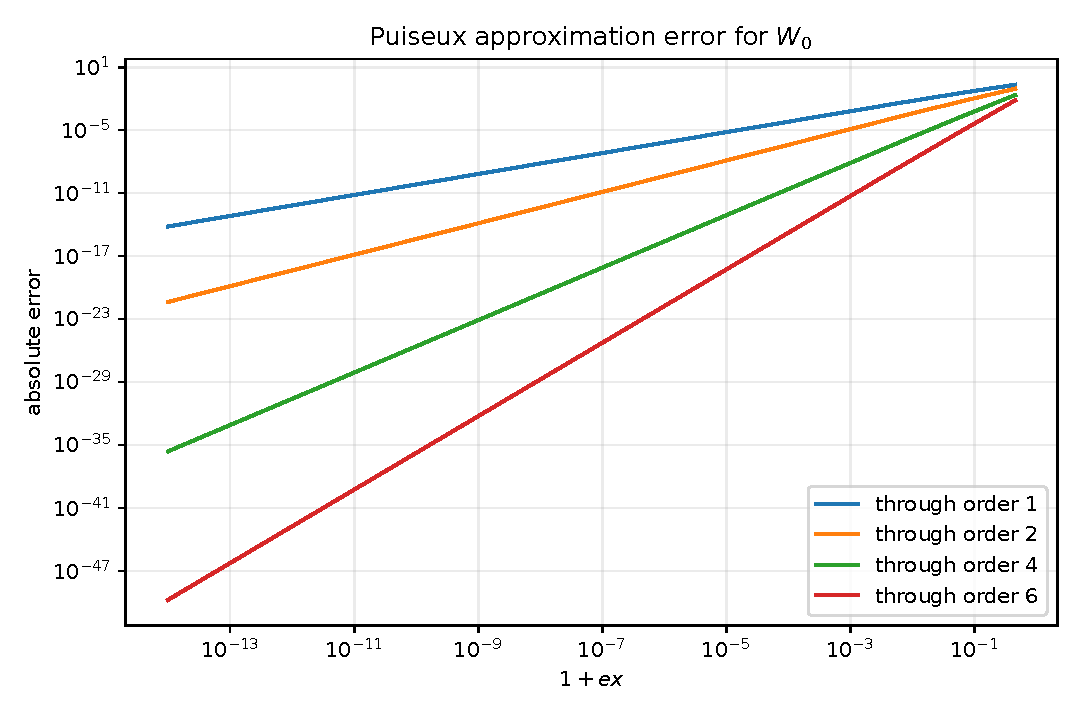
\includegraphics[width=.78\textwidth]{branch_point_error_W0.pdf}
\caption{Absolute errors of successive truncations of
\eqref{eq:puiseux-series} on the principal branch.}
\label{fig:brancherr0}
\end{figure}

\begin{figure}[H]
\centering
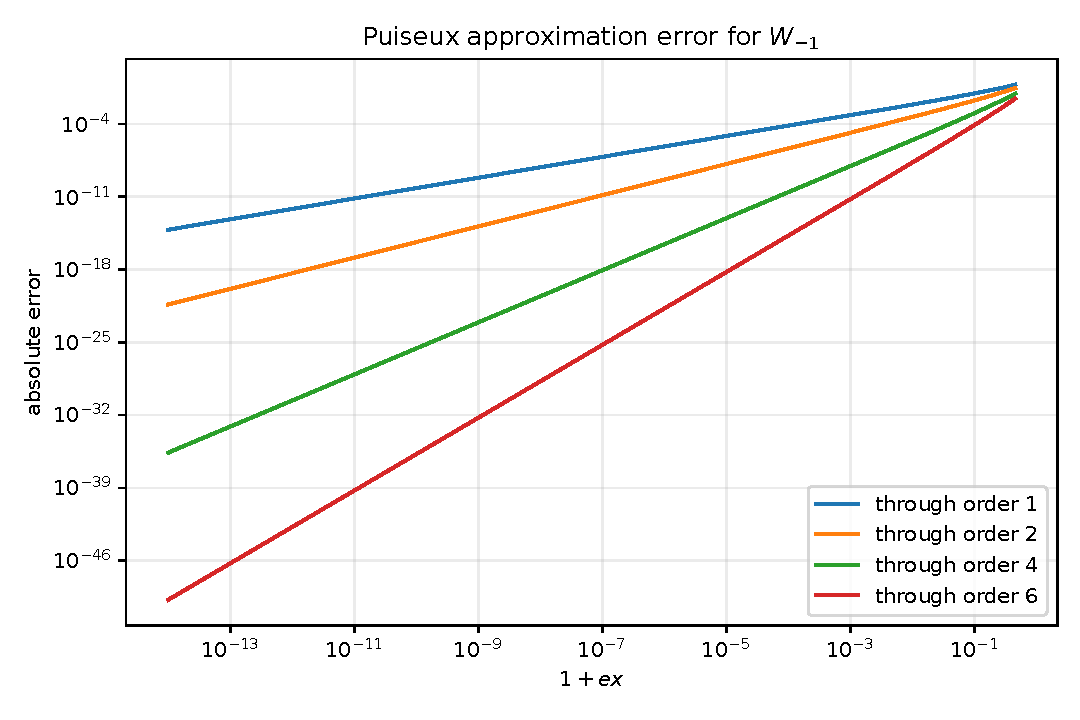
\includegraphics[width=.78\textwidth]{branch_point_error_Wm1.pdf}
\caption{The same signed expansion, now with \(p<0\), approximates
the nonprincipal branch.}
\label{fig:brancherrm}
\end{figure}

\subsection{An exponential branch-point coordinate}

A second useful parametrization is
\begin{equation}\label{eq:tparamx}
       x=-\EulerE^{-1-t^2/2}.
\end{equation}
Choose \(t>0\) for \(W_0\) and \(t<0\) for \(W_{-1}\).  If
\(W=-1+u\), then the defining equation becomes
\[
       (1-u)\EulerE^u=\EulerE^{-t^2/2},
\]
or
\begin{equation}\label{eq:t-u-relation}
       \frac{t^2}{2}=-u-\log(1-u).
\end{equation}
The right side begins with \(u^2/2\), so another inverse-series calculation
gives
\begin{equation}\label{eq:tseries}
 W=-1+t-\frac13t^2+\frac1{36}t^3+\frac1{270}t^4
      +\frac1{4320}t^5-\frac1{17010}t^6+\BigO(t^7).
\end{equation}
The proof is identical in structure to that of
\cref{thm:puiseux}: the signed analytic square root of
\(2[-u-\log(1-u)]\) has derivative \(1\) at the origin and therefore has a
local analytic inverse.

\begin{literaturenote}
The NIST DLMF~\cite{dlmf} and the foundational paper of Corless et
al.~\cite{corless1996} tabulate many more branch-point coefficients.  The exponential coordinate
\eqref{eq:tparamx} is particularly convenient in rigorous numerical work,
because \(t^2/2=-1-\log(-x)\) is computed accurately even when \(x\) is
represented in logarithmic form.
\end{literaturenote}

\section{Logarithmic asymptotic expansions}\label{sec:asymptotics}

The two unbounded real limits are
\[
       \Wz(x)\longrightarrow+\infty\quad(x\to+\infty),
       \qquad
       \Wm(x)\longrightarrow-\infty\quad(x\to0^-).
\]
They are governed by the same algebra.  The first approximation follows by
taking logarithms:
\[
       W+\log\AbsoluteValue W=\log\AbsoluteValue x.
\]
If \(\AbsoluteValue W\) is large, then \(W\) is approximately \(\log\AbsoluteValue x\), and a
second approximation subtracts the logarithm of that first approximation.

\subsection{Unsigned Stirling numbers}

The unsigned Stirling number of the first kind
\(\stirling{n}{j}\) is defined by
\begin{equation}\label{eq:stirling-def}
 t(t+1)\cdots(t+n-1)
 =\sum_{j=0}^n\stirling{n}{j}t^j.
\end{equation}
It counts permutations of \(n\) objects having \(j\) cycles, but only its
algebraic role is needed here.  The recurrence
\begin{equation}\label{eq:stirling-rec}
 \stirling{n}{j}
 =\stirling{n-1}{j-1}+(n-1)\stirling{n-1}{j}
\end{equation}
follows by multiplying the product for \(n-1\) by \(t+n-1\).

\begin{lemma}[Exponential generating function]\label{lem:stirling-egf}
For \(r\geq0\),
\begin{equation}\label{eq:stirling-egf}
 \frac{[-\log(1-z)]^r}{r!}
 =\sum_{n=r}^{\infty}\stirling{n}{r}\frac{z^n}{n!},
 \qquad |z|<1.
\end{equation}
Consequently,
\begin{equation}\label{eq:stirling-derivative-egf}
 \frac{[-\log(1-z)]^r}{r!(1-z)}
 =\sum_{n=r}^{\infty}
   \stirling{n+1}{r+1}\frac{z^n}{n!}.
\end{equation}
\end{lemma}

\begin{proof}
Let the right side of \eqref{eq:stirling-egf} be \(F_r(z)\).
Using \eqref{eq:stirling-rec} and shifting indices shows
\[
       F_r'(z)=\frac{F_{r-1}(z)}{1-z},\qquad F_r(0)=0
       \quad(r\geq1),
\]
while \(F_0(z)=1\).  The functions
\([-\log(1-z)]^r/r!\) satisfy the same differential recurrence and initial
conditions, so induction on \(r\) proves \eqref{eq:stirling-egf}.
Differentiate the formula with \(r+1\) in place of \(r\) to obtain
\eqref{eq:stirling-derivative-egf}.
\end{proof}

Define polynomials
\begin{equation}\label{eq:Pn-asym}
 \mathcal P_n(L)
 =\sum_{m=1}^n
   \frac{(-1)^{n-m}}{m!}
   \stirling{n}{n-m+1}L^m.
\end{equation}
The first four are
\begin{align}
 \mathcal P_1(L)&=L,\label{eq:P1}\\
 \mathcal P_2(L)&=\frac{L(-2+L)}2,\label{eq:P2}\\
 \mathcal P_3(L)&=\frac{L(6-9L+2L^2)}6,\label{eq:P3}\\
 \mathcal P_4(L)&=\frac{L(-12+36L-22L^2+3L^3)}{12}.
 \label{eq:P4}
\end{align}

\begin{theorem}[Unified complete real asymptotic expansion]\label{thm:fullasym}
For either of the following limits,
\[
 \begin{array}{c|c|c}
 \text{branch and limit}&L_1&L_2\\ \hline
 \Wz(x),\ x\to+\infty&\log x&\log\log x\\
 \Wm(x),\ x\to0^-&\log(-x)&\log[-\log(-x)]
 \end{array}
\]
one has, for every fixed \(N\geq1\),
\begin{equation}\label{eq:fullasym}
 W(x)=L_1-L_2+
 \sum_{n=1}^{N}\frac{\mathcal P_n(L_2)}{L_1^n}
 +\BigO\left(
 \frac{L_2^{N+1}}{\AbsoluteValue{L_1}^{N+1}}
 \right).
\end{equation}
Equivalently, the formal complete expansion is
\begin{equation}\label{eq:doubleasym}
 W(x)\sim L_1-L_2+
 \sum_{k=0}^{\infty}\sum_{m=1}^{\infty}
 \frac{(-1)^k}{m!}
 \stirling{k+m}{k+1}
 \frac{L_2^m}{L_1^{k+m}}.
\end{equation}
\end{theorem}

\begin{proof}
Set
\[
       W=L_1-L_2+v,\qquad
       \sigma=\frac1{L_1},\qquad
       \tau=\frac{L_2}{L_1}.
\]
For the principal positive branch,
\(\log x=W+\log W\).  Factoring \(L_1\) from \(W\) gives
\[
 0=v+\log(1-\tau+\sigma v).
\]
For the negative branch, \(\log(-x)=W+\log(-W)\); because \(L_1<0\),
factoring \(-L_1\) from \(-W\) gives exactly the same equation.  Hence
\begin{equation}\label{eq:vimplicit}
       \tau=1-\EulerE^{-v}+\sigma v.
\end{equation}

Apply Lagrange inversion to the inverse of the right side:
\begin{align}
 v
 &=\sum_{m=1}^{\infty}\frac{\tau^m}{m}
 [t^{m-1}]
 \left(\frac{t}{1-\EulerE^{-t}+\sigma t}\right)^m\notag\\
 &=\sum_{m=1}^{\infty}\sum_{k=0}^{\infty}
 \frac{(-1)^k}{m}
 \binom{m+k-1}{k}\sigma^k\tau^m
 [t^{m-1}]
 \left(\frac{t}{1-\EulerE^{-t}}\right)^{m+k}.
 \label{eq:asym-lagrange}
\end{align}
We claim that
\begin{equation}\label{eq:keycoeff-asym}
 [t^{m-1}]
 \left(\frac{t}{1-\EulerE^{-t}}\right)^{m+k}
 =\frac{k!}{(m+k-1)!}\stirling{m+k}{k+1}.
\end{equation}
To prove it, write the coefficient as a formal residue:
\[
 \ResidueOperator_{t=0}\frac{t^k}{(1-\EulerE^{-t})^{m+k}}\Differential t.
\]
Make the substitution \(z=1-\EulerE^{-t}\), so
\(t=-\log(1-z)\) and \(\Differential t=\Differential z/(1-z)\).  The residue becomes the
coefficient of \(z^{m+k-1}\) in
\[
       \frac{[-\log(1-z)]^k}{1-z}.
\]
Formula \eqref{eq:stirling-derivative-egf} says that this coefficient is the
right side of \eqref{eq:keycoeff-asym}.

Substitution into \eqref{eq:asym-lagrange} simplifies the numerical factor:
\[
 \frac1m\binom{m+k-1}{k}\frac{k!}{(m+k-1)!}
 =\frac1{m!}.
\]
Therefore
\[
 v=\sum_{m\geq1}\sum_{k\geq0}
 \frac{(-1)^k}{m!}\stirling{m+k}{k+1}
 \sigma^k\tau^m.
\]
Since \(\sigma^k\tau^m=L_2^m/L_1^{k+m}\), this is
\eqref{eq:doubleasym}; collecting terms with \(k+m=n\) gives
\eqref{eq:Pn-asym}.

Finally, the implicit function in \eqref{eq:vimplicit} has derivative \(1\)
with respect to \(v\) at \((v,\sigma,\tau)=(0,0,0)\).  Hence \(v\) is
analytic in \((\sigma,\tau)\) near the origin.  Its Taylor remainder after
total degree \(N\) is
\(\BigO((|\sigma|+|\tau|)^{N+1})\).  In both limits,
\(\sigma\to0\), \(\tau\to0\), and
\(|\tau|=L_2/|L_1|\) eventually dominates \(|\sigma|\).  This proves the
remainder estimate in \eqref{eq:fullasym}.
\end{proof}

\subsection{The expansion written separately for each branch}

For \(x\to+\infty\), set \(A=\log x\) and \(B=\log A\).  Then
\begin{align}
 \Wz(x)={}&A-B+\frac{B}{A}
 +\frac{B(-2+B)}{2A^2}
 +\frac{B(6-9B+2B^2)}{6A^3}\notag\\
 &+\frac{B(-12+36B-22B^2+3B^3)}{12A^4}
 +\BigO\left(\frac{B^5}{A^5}\right).
 \label{eq:asymW0explicit}
\end{align}

For \(x\to0^-\), set
\[
       \eta=\log\frac1{-x},\qquad B=\log\eta.
\]
Since \(L_1=-\eta\),
\begin{align}
 \Wm(x)={}&-\eta-B-\frac{B}{\eta}
 +\frac{B(B-2)}{2\eta^2}
 -\frac{B(2B^2-9B+6)}{6\eta^3}\notag\\
 &+\frac{B(3B^3-22B^2+36B-12)}{12\eta^4}
 +\BigO\left(\frac{B^5}{\eta^5}\right).
 \label{eq:asymWmexplicit}
\end{align}

\begin{figure}[H]
\centering
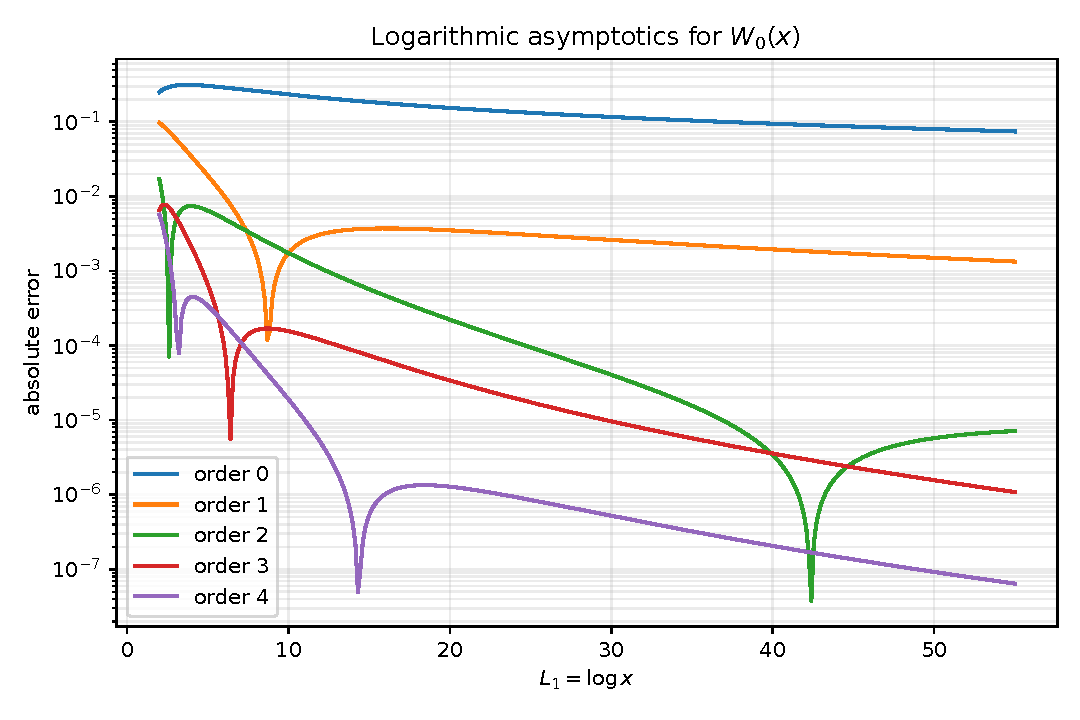
\includegraphics[width=.78\textwidth]{asymptotic_error_W0.pdf}
\caption{Truncation errors in the logarithmic expansion for \(\Wz\).
The horizontal coordinate is \(A=\log x\), so the right edge represents
astronomically large \(x\).}
\label{fig:asym0}
\end{figure}

\begin{figure}[H]
\centering
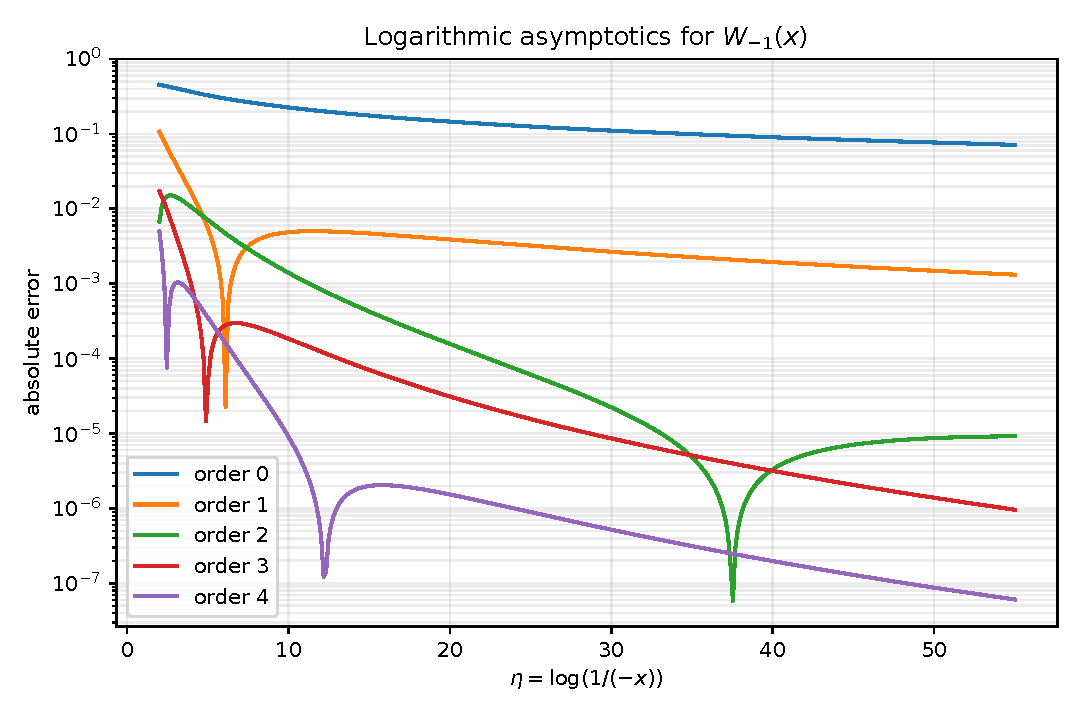
\includegraphics[width=.78\textwidth]{asymptotic_error_Wm1.pdf}
\caption{The same coefficient polynomials approximate \(\Wm(x)\) as
\(x\to0^-\), after the sign of \(L_1\) is changed.}
\label{fig:asymm}
\end{figure}

\begin{remark}[Asymptotic does not mean ``keep every term'']
For a fixed moderate argument, adding terms can eventually stop improving an
asymptotic approximation.  One should compare successive terms and stop near
the smallest one.  For genuinely large \(|L_1|\), however, each fixed-order
truncation in \cref{thm:fullasym} has the proved error order shown there.
\end{remark}



\section{Rigorous elementary bounds}\label{sec:bounds}

Bounds serve three purposes: they explain the shape of the graph, provide
quick approximations, and furnish guaranteed starting values for iteration.

\begin{lemma}[Two logarithm inequalities]\label{lem:logineq}
For \(t>-1\),
\begin{equation}\label{eq:logineq}
       \frac{t}{1+t}\leq\log(1+t)\leq t,
\end{equation}
with equality only at \(t=0\).
\end{lemma}

\begin{proof}
For the upper bound, let \(g(t)=t-\log(1+t)\).  Then
\(g'(t)=t/(1+t)\), so \(g\) decreases to \(g(0)=0\) on \((-1,0)\) and
increases from \(0\) on \((0,\infty)\).  Thus \(g\geq0\).

For the lower bound, let
\(h(t)=\log(1+t)-t/(1+t)\).  Then
\(h'(t)=t/(1+t)^2\).  The same monotonicity argument gives \(h\geq0\).
\end{proof}

\subsection{Bounds for the principal branch on \texorpdfstring{\(x\geq0\)}{x >= 0}}

\begin{theorem}[Global elementary principal-branch bounds]\label{thm:W0positivebounds}
For every \(x\geq0\),
\begin{equation}\label{eq:W0positivebounds}
 \boxed{\displaystyle
 \frac{x}{1+x}\leq\Wz(x)\leq\log(1+x)\leq x.}
\end{equation}
All inequalities are strict when \(x>0\), except where an accidental equality
is forced at \(x=0\).
\end{theorem}

\begin{proof}
Let \(w=\Wz(x)\geq0\), so \(x=w\EulerE^w\).  The elementary inequality
\(1-\EulerE^{-w}\leq w\) is equivalent both to
\[
       \frac{x}{1+x}\leq w
\]
and to
\[
       \EulerE^w\leq1+x,
\]
the latter being \(w\leq\log(1+x)\).  Finally
\(\log(1+x)\leq x\) is \cref{lem:logineq}.
\end{proof}

The first rational lower bound is also the \([1/1]\) Pade approximant of
\(\Wz\) at the origin.  Its role is therefore both analytic and numerical.

\begin{theorem}[Logarithmic bounds for large positive arguments]\label{thm:W0logbounds}
Let \(x>\EulerE\), \(L=\log x>1\).  Then
\begin{equation}\label{eq:W0logbounds}
 L-\log L
 <\Wz(x)
 <L-\log(L-\log L)
 <L.
\end{equation}
At \(x=\EulerE\), the first lower bound is an equality:
\(\Wz(\EulerE)=1\).
\end{theorem}

\begin{proof}
The function \(f(w)=w\EulerE^w\) is increasing for \(w>0\).  Since
\[
       L\EulerE^L=Lx>x,
\]
we have \(W_0(x)<L\).  Put \(a=L-\log L>0\).  Then
\[
       a\EulerE^a
       =(L-\log L)\frac{x}{L}
       =x\left(1-\frac{\log L}{L}\right)<x,
\]
so \(a<W_0(x)\).  The equation \(W_0=L-\log W_0\) and the lower bound
\(W_0>a\) imply
\[
       W_0=L-\log W_0<L-\log a.
\]
Finally, the function \(h(L)=L-\log L\) is strictly increasing for
\(L>1\), and \(h(1)=1\).  Thus \(a=h(L)>1\), so \(\log a>0\) and
\(L-\log a<L\).
\end{proof}

Repeated use of the decreasing map \(g(w)=L-\log w\) produces alternating
upper and lower bounds.  For example, starting with
\[
       \ell_0=L-\log L,\qquad u_0=L,
\]
the implication
\[
       \ell\leq W_0\leq u
       \quad\Longrightarrow\quad
       L-\log u\leq W_0\leq L-\log\ell
\]
follows immediately from the fact that \(g\) is decreasing.

\subsection{Bounds on the negative part of the principal branch}

\begin{theorem}[Two square-root bounds and a linear bound]\label{thm:W0negativebounds}
For \(-1/\EulerE<x<0\),
\begin{equation}\label{eq:W0negativebounds}
 -1+\sqrt{1+\EulerE x}
 <\Wz(x)
 <-1+\sqrt{2(1+\EulerE x)},
\end{equation}
and also
\begin{equation}\label{eq:W0xbound}
       \Wz(x)<x.
\end{equation}
The first lower bound becomes exact at both endpoints in the limiting sense.
\end{theorem}

\begin{proof}
Write \(w=-1+s\) with \(0<s<1\).  Then
\[
       1+\EulerE x=1+(s-1)\EulerE^s.
\]
The lower inequality is equivalent to
\[
       s^2>1+(s-1)\EulerE^s.
\]
Since \(s-1<0\), this in turn is equivalent to
\(1+s<\EulerE^s\), which is strict for \(s>0\).

For the upper square-root bound, define
\[
 H(s)=2[1-(1-s)\EulerE^s]-s^2.
\]
Then \(H(0)=0\) and
\[
       H'(s)=2s(\EulerE^s-1)>0
\]
for \(s>0\).  Thus
\(s^2<2(1+\EulerE x)\), proving the upper bound.

Finally \(x=w\EulerE^w\).  Since \(w<0\) and \(0<\EulerE^w<1\), multiplication of
the negative number \(w\) by \(\EulerE^w\) moves it toward zero, so \(w<x\).
\end{proof}

Near \(x=0\), the bound \(W_0(x)<x\) is much sharper than the upper
square-root bound; near the branch point, the square-root bounds reveal the
correct scale.

\subsection{Bounds for the nonprincipal branch near the branch point}

The following result, due to Chatzigeorgiou~\cite{chatzigeorgiou2013}, is
particularly useful because its proof needs only elementary inequalities.

\begin{theorem}[Two-sided \(W_{-1}\) bound]\label{thm:chatzbound}
For \(u>0\),
\begin{equation}\label{eq:chatzbound}
 \boxed{\displaystyle
 -1-\sqrt{2u}-u
 <\Wm(-\EulerE^{-1-u})
 <-1-\sqrt{2u}-\frac23u.}
\end{equation}
\end{theorem}

\begin{proof}
Write
\[
       \Wm(-\EulerE^{-1-u})=-1-v,\qquad v>0.
\]
The defining equation gives
\[
       (1+v)\EulerE^{-v}=\EulerE^{-u},
\]
hence
\begin{equation}\label{eq:u-v}
       u=v-\log(1+v).
\end{equation}
The desired inequalities are equivalent to
\begin{equation}\label{eq:v-bounds}
       \sqrt{2u}+\frac23u<v<\sqrt{2u}+u.
\end{equation}

For the upper bound, \(v-u=\log(1+v)\).  Put
\(t=\log(1+v)>0\), so \(v=\EulerE^t-1\) and
\(u=\EulerE^t-1-t\).  The strict exponential inequality
\(\EulerE^t>1+t+t^2/2\) gives
\[
       t<\sqrt{2u},
\]
and hence \(v=u+t<u+\sqrt{2u}\).

For the lower bound, note first that \(v-\frac23u=(v+2t)/3>0\).
It is therefore enough to square.  The required inequality is equivalent to
\[
       (v+2t)^2>18u.
\]
Substituting \(v=\EulerE^t-1\) and \(u=\EulerE^t-1-t\), define
\[
 F(t)=(\EulerE^t-1+2t)^2-18(\EulerE^t-1-t).
\]
A direct differentiation gives
\[
 F(0)=F'(0)=F''(0)=F'''(0)=0,
\]
and
\[
       F^{(4)}(t)=4\EulerE^t(t+4\EulerE^t-1)>0\qquad(t>0).
\]
Successive integrations from \(0\) show
\(F'''(t)>0\), then \(F''(t)>0\), then \(F'(t)>0\), and finally
\(F(t)>0\).  This proves the lower inequality in
\eqref{eq:v-bounds}, and therefore \eqref{eq:chatzbound}.
\end{proof}

\begin{corollary}[A one-line branch-point approximation]\label{cor:Wm-midpoint}
With \(u=-1-\log(-x)>0\), define
\begin{equation}\label{eq:Wm-midpoint}
 A_{-1}(x)=-1-\sqrt{2u}-\frac56u.
\end{equation}
Then
\begin{equation}\label{eq:Wm-midpoint-error}
       \AbsoluteValue{\Wm(x)-A_{-1}(x)}<\frac{u}{6}.
\end{equation}
\end{corollary}

\begin{proof}
The approximation is the midpoint of the two bounds in
\eqref{eq:chatzbound}; their distance is \(u/3\).
\end{proof}

\begin{figure}[H]
\centering
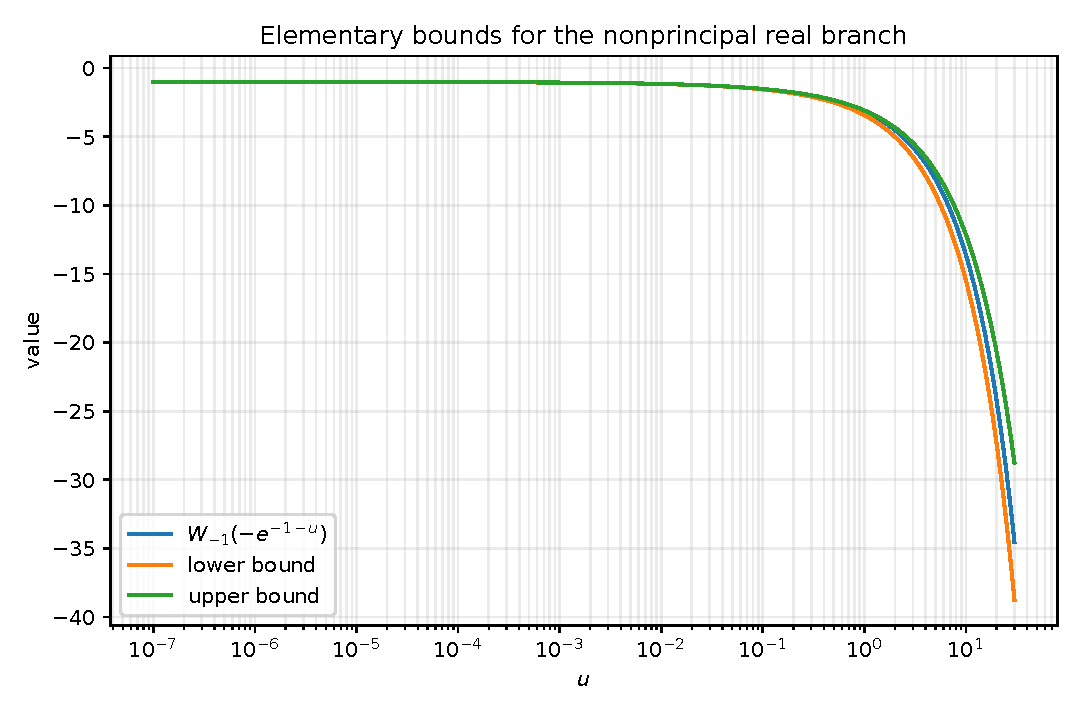
\includegraphics[width=.78\textwidth]{Wm1_bounds.pdf}
\caption{The two elementary bounds of \cref{thm:chatzbound}.  They are
especially effective near \(u=0\), which is the branch point.}
\label{fig:Wmbounds}
\end{figure}

A simpler square-root consequence, useful when only \(x\) is available, is
\[
       \Wm(x)<-1-\sqrt{2(1+\EulerE x)}.
\]
Indeed, with \(w=-1-v\),
\[
 v^2-2[1-(1+v)\EulerE^{-v}]
\]
has derivative \(2v(1-\EulerE^{-v})>0\) and vanishes at \(v=0\).

\subsection{Bounds for \texorpdfstring{\(W_{-1}\)}{W-1} near zero}

The preceding \(u\)-bounds capture the branch point.  A different pair
captures the logarithmic singularity.

\begin{theorem}[Near-zero logarithmic bounds]\label{thm:Wmzerobounds}
Let \(-1/\EulerE<x<0\), and put
\[
       \eta=\log\frac1{-x}>1.
\]
Then
\begin{equation}\label{eq:Wmzerobounds}
 -\eta-\frac{\eta\log\eta}{\eta-1}
 \leq\Wm(x)
 <-\eta-\log\eta.
\end{equation}
\end{theorem}

\begin{proof}
Let \(y=-\Wm(x)>1\).  Then
\[
       y-\log y=\eta,\qquad\text{or}\qquad y=\eta+\log y.
\]
Since \(y>\eta\), one has
\[
       y>\eta+\log\eta,
\]
which gives the upper bound for \(\Wm=-y\).

For the other direction, set
\[
       B=\eta+\frac{\eta\log\eta}{\eta-1}
       =\eta+r,\qquad
       r=\frac{\eta\log\eta}{\eta-1}.
\]
Because \(\log(1+s)\leq s\),
\[
 \log B
 =\log\eta+\log\left(1+\frac r\eta\right)
 \leq\log\eta+\frac r\eta
 =r.
\]
Thus \(B-\log B\geq\eta\).  The function
\(z-\log z\) is strictly increasing for \(z>1\), and
\(y-\log y=\eta\), so \(y\leq B\).  Multiplying by \(-1\) proves the lower
bound in \eqref{eq:Wmzerobounds}.
\end{proof}

The interval width in \eqref{eq:Wmzerobounds} is
\[
       \frac{\log\eta}{\eta-1},
\]
which tends to zero.  Thus the two leading terms
\(-\eta-\log\eta\) are not merely asymptotically plausible; they are enclosed
by an elementary shrinking bracket.

\section{Rational and continued-fraction approximations}\label{sec:rational}

\subsection{Pade approximants at the origin}

A \([r/s]\) Pade approximant is a rational function \(P_r(x)/Q_s(x)\)
whose Taylor series agrees with the target through as many terms as possible,
with \(Q_s(0)=1\).  Solving the resulting linear coefficient equations for
\(\Wz\) gives
\begin{align}
 R_{1,1}(x)&=\frac{x}{1+x},\label{eq:pade11}\\
 R_{2,2}(x)&=\frac{2x(4x+3)}{5x^2+14x+6},\label{eq:pade22}\\
 R_{3,3}(x)&=
 \frac{3x(451x^2+912x+340)}
 {665x^3+3579x^2+3756x+1020}.\label{eq:pade33}
\end{align}

\begin{proposition}[Orders of contact]\label{prop:pade-errors}
At the origin,
\begin{align}
 \Wz(x)-R_{1,1}(x)&=\frac12x^3+\BigO(x^4),\\
 \Wz(x)-R_{2,2}(x)&=\frac{17}{72}x^5+\BigO(x^6),\\
 \Wz(x)-R_{3,3}(x)&=\frac{13489}{122400}x^7+\BigO(x^8).
\end{align}
None of these three rational functions has a pole on the real domain
\([-1/\EulerE,\infty)\) of \(\Wz\).
\end{proposition}

\begin{proof}
Expand each denominator as a geometric power series at zero, multiply by its
numerator, and compare with \eqref{eq:Wseries}.  This gives the displayed
first unmatched terms.  For \(R_{1,1}\), the only pole is \(-1\).  The roots
of the quadratic denominator in \(R_{2,2}\) are
\[
       \frac{-7\pm\sqrt{19}}5,
\]
and both are less than \(-1/\EulerE\).

For the cubic denominator, write
\[
       D(x)=665x^3+3579x^2+3756x+1020.
\]
The exponential series gives \(\EulerE>8/3\), hence
\(-1/\EulerE>-3/8\).  On \([-3/8,\infty)\), the quadratic
\[
       \frac{D'(x)}3=665x^2+2386x+1252
\]
is increasing, because its derivative \(1330x+2386\) is positive there;
its value at \(-3/8\) is \(28849/64>0\).  Thus \(D\) is increasing on
that interval, and
\[
       D(-3/8)=\frac{40821}{512}>0.
\]
It follows that \(D(x)>0\) for every \(x\geq-1/\EulerE\).  Hence the cubic
approximant has no pole on the principal real domain.
\end{proof}

\begin{figure}[H]
\centering
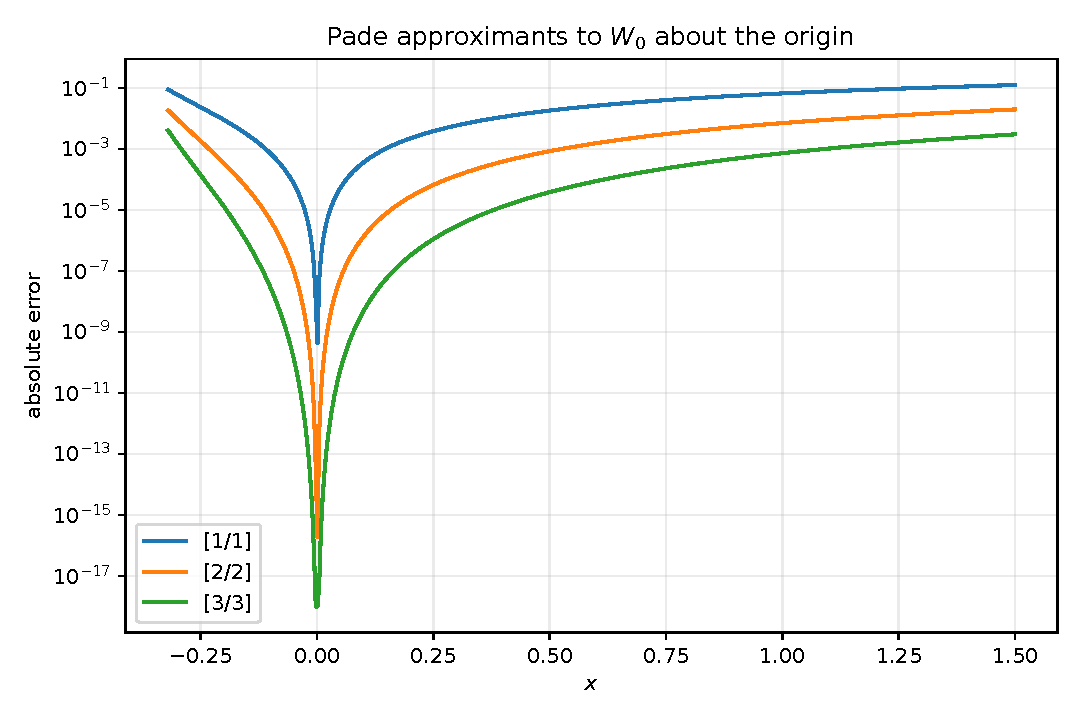
\includegraphics[width=.78\textwidth]{pade_errors.pdf}
\caption{Absolute errors of three diagonal Pade approximants.  Their main
advantage over a Taylor polynomial is sensible behavior beyond the disk
\(\AbsoluteValue{x}<1/\EulerE\).}
\label{fig:pade}
\end{figure}

These approximants belong naturally to \(W_0\).  The branch \(W_{-1}\) has
no Taylor series at \(x=0\); for it, one should first use the branch-point
variable \(p\), the exponential variable \(t\), or the logarithmic variable
\(\eta\), and then approximate the transformed function.

\subsection{Euler's continued fraction}

For a generalized continued fraction, write
\[
 b_0+\underset{n=1}{\mathbf K^N}\frac{\alpha_n}{\beta_n}
 =
 b_0+\cfrac{\alpha_1}{\beta_1+
       \cfrac{\alpha_2}{\beta_2+\cdots+
       \cfrac{\alpha_N}{\beta_N}}}.
\]

\begin{lemma}[Euler connection]\label{lem:euler-cf}
Let \(c_0,c_1,\ldots\) be nonzero where ratios are used, and put
\(r_n=c_n/c_{n-1}\).  The \(N\)-th convergent of
\begin{equation}\label{eq:euler-general}
 c_0+\cfrac{c_1}{1+
   \underset{n=2}{\mathbf K^N}
   \frac{-r_n}{1+r_n}}
\end{equation}
is exactly the partial sum \(\sum_{n=0}^Nc_n\).
\end{lemma}

\begin{proof}
The numerator and denominator continuants \(P_n,Q_n\) of a generalized
continued fraction obey
\[
 P_n=\beta_nP_{n-1}+\alpha_nP_{n-2},\qquad
 Q_n=\beta_nQ_{n-1}+\alpha_nQ_{n-2}.
\]
This recurrence follows by clearing the last denominator in the nested
fraction.  Here
\[
 \alpha_1=c_1,\quad\beta_1=1,\qquad
 \alpha_n=-r_n,\quad\beta_n=1+r_n\quad(n\geq2),
\]
with \(P_0=c_0,Q_0=1\).  The first convergent is
\(P_1/Q_1=c_0+c_1\).  If
\(P_{n-1}=\sum_{j=0}^{n-1}c_j\),
\(P_{n-2}=\sum_{j=0}^{n-2}c_j\), and
\(Q_{n-1}=Q_{n-2}=1\), then
\[
 P_n=(1+r_n)\sum_{j=0}^{n-1}c_j
      -r_n\sum_{j=0}^{n-2}c_j
    =\sum_{j=0}^{n-1}c_j+r_nc_{n-1}
    =\sum_{j=0}^nc_j,
\]
while \(Q_n=(1+r_n)-r_n=1\).  Induction proves the claim.
\end{proof}

For the Lambert series, let
\[
       c_n=\frac{(-n)^{n-1}}{n!}x^n\qquad(n\geq1).
\]
A calculation gives
\[
 \frac{c_n}{c_{n-1}}
 =-\left(1-\frac1n\right)^{2-n}x=:a_nx.
\]

\begin{theorem}[Euler continued fraction for \(W_0\)]\label{thm:eulerW}
For \(\AbsoluteValue{x}<1/\EulerE\),
\begin{equation}\label{eq:eulerW}
 \boxed{\displaystyle
 \Wz(x)=
 \frac{x}{
  1+\underset{n=2}{\mathbf K^\infty}
  \frac{-a_nx}{1+a_nx}},
 \qquad
 a_n=-\left(1-\frac1n\right)^{2-n}.}
\end{equation}
The convergents are exactly the partial sums of the Maclaurin series.
\end{theorem}

\begin{proof}
Apply \cref{lem:euler-cf} with \(c_0=0\) and the displayed ratios.
Each convergent equals a Maclaurin partial sum, and those partial sums
converge to \(\Wz(x)\) for \(\AbsoluteValue{x}<1/\EulerE\).
\end{proof}

\begin{literaturenote}
The paper of Corcino, Corcino, and Mez\H{o} in the supplied archive develops
more sophisticated regular and associated continued fractions, including
coefficient formulas through Hankel determinants and numerical studies of
their convergence.  Formula \eqref{eq:eulerW} is the elementary Euler
connection from which that discussion begins.
\end{literaturenote}


\section{Contour and real integral representations}\label{sec:integralreps}

Integral representations are useful for proofs of monotonicity, for
quadrature, and for connecting \(W\) with complex analysis.  We begin with a
formula that applies to every branch.

\subsection{A local contour representation for all branches}

\begin{theorem}[Inverse-function residue formula]\label{thm:contour-all}
Let \(z\) be a regular value of \(f(\zeta)=\zeta\EulerE^\zeta\), and let
\(\Gamma_k\) be a small positively oriented contour enclosing the one simple
root \(\zeta=W_k(z)\) and no other root of \(f(\zeta)=z\).  Then, for every
integer \(m\geq0\),
\begin{equation}\label{eq:contour-all}
 W_k(z)^m
 =\frac{1}{2\pi\ImaginaryUnit}\int_{\Gamma_k}
 \frac{\zeta^m\EulerE^\zeta(1+\zeta)}
      {\zeta\EulerE^\zeta-z}\Differential\zeta.
\end{equation}
For \(m=1\), this is an integral representation of \(W_k(z)\) itself.
\end{theorem}

\begin{proof}
The denominator has a simple zero at \(\zeta=W_k(z)\), because
\(f'(\zeta)=\EulerE^\zeta(1+\zeta)\neq0\) at a regular value.  The residue of the
integrand there is
\[
 \frac{\zeta^m f'(\zeta)}{f'(\zeta)}
 \bigg|_{\zeta=W_k(z)}
 =W_k(z)^m.
\]
The residue theorem proves the formula.
\end{proof}

This representation includes \(W_{-1}\) whenever a contour isolates that
preimage.  What follows is more special: a positive real integral for the principal
branch, in the family studied by Kalugin, Jeffrey, and
Corless~\cite{kalugin2012}.

\subsection{The principal-branch cut parametrization}

For \(0<v<\pi\), define
\begin{equation}\label{eq:av}
       a(v)=v\EulerE^{-v\cot v}\csc v.
\end{equation}

\begin{lemma}[Properties of \(a(v)\)]\label{lem:av}
The function \(a\) is strictly increasing and maps \((0,\pi)\) onto
\((1/\EulerE,\infty)\).  Moreover,
\begin{equation}\label{eq:aderivative}
 \frac{v a'(v)}{a(v)}
 =1-2v\cot v+v^2\csc^2v
 =(1-v\cot v)^2+v^2>0.
\end{equation}
\end{lemma}

\begin{proof}
Taking logarithms of \eqref{eq:av} and differentiating gives
\[
 \frac{a'}a=\frac1v-2\cot v+v\csc^2v,
\]
which is \eqref{eq:aderivative}.  Its final expression is positive.

As \(v\to0\), the expansions
\(\sin v\sim v\) and \(v\cot v\to1\) give \(a(v)\to1/\EulerE\).
As \(v\to\pi^-\), one has \(\csc v\to+\infty\) and
\(-v\cot v\to+\infty\), so \(a(v)\to\infty\).  Strict monotonicity now gives
the claimed range.
\end{proof}

Why does this function appear?  On the upper edge of the principal branch
cut, write
\[
       W_0(-a+\ImaginaryUnit0)=u+\ImaginaryUnit v,\qquad 0<v<\pi.
\]
The condition that \((u+\ImaginaryUnit v)\EulerE^{u+\ImaginaryUnit v}\) be negative real forces
\[
       u=-v\cot v,
\]
and its real value is
\[
       -v\EulerE^{-v\cot v}\csc v=-a(v).
\]
Thus \(v\) parametrizes the entire cut from \(-1/\EulerE\) to \(-\infty\).

\begin{theorem}[Stieltjes and logarithmic integrals]\label{thm:stieltjes}
For \(z\in\ComplexNumbers\setminus(-\infty,-1/\EulerE]\),
\begin{align}
 W_0'(z)
 &=\frac1\pi\int_0^\pi\frac{\Differential v}{z+a(v)},\label{eq:Wprime-stieltjes}\\
 W_0(z)
 &=\frac1\pi\int_0^\pi
   \PrincipalLogarithm\left(1+\frac{z}{a(v)}\right)\Differential v,\label{eq:W-log-integral}\\
 W_0(z)
 &=\frac{z}{\pi}\int_0^\pi
 \frac{(1-v\cot v)^2+v^2}{z+a(v)}\Differential v.
 \label{eq:W-stieltjes}
\end{align}
For real \(z>-1/\EulerE\), all three integrals are real and the ordinary real
logarithm may be used in \eqref{eq:W-log-integral}.
\end{theorem}

\begin{proof}
We first prove \eqref{eq:Wprime-stieltjes}.  Let
\(F(z)=W_0'(z)\).  It is analytic off the cut, behaves as
\(\BigO(1/z)\) at infinity, and has an integrable inverse-square-root
singularity at \(-1/\EulerE\).  On the upper edge of the cut,
\[
       W_0(-a(v)+\ImaginaryUnit0)=-v\cot v+\ImaginaryUnit v.
\]
Differentiating with respect to \(v\), while
\(z=-a(v)\), gives
\[
 F(-a(v)+\ImaginaryUnit0)
 =-\frac{(-v\cot v)'+\ImaginaryUnit}{a'(v)}.
\]
The lower boundary value is its complex conjugate.  Hence the jump is
\begin{equation}\label{eq:Fjump}
       F_+-F_-=-\frac{2\ImaginaryUnit}{a'(v)}.
\end{equation}

Apply Cauchy's formula on a large keyhole contour surrounding the cut.
The outer circle contributes zero in the limit because
\(F(z)=\BigO(1/z)\); a small circle around the branch point contributes zero
because its length is order \(r\) and \(F\) is order \(r^{-1/2}\).
The two sides of the cut therefore give
\[
 F(z)=\frac1{2\pi\ImaginaryUnit}
 \int_{-\infty}^{-1/\EulerE}
 \frac{F_+(t)-F_-(t)}{t-z}\Differential t.
\]
Set \(t=-a(v)\).  As \(t\) runs from \(-\infty\) to \(-1/\EulerE\),
\(v\) runs from \(\pi\) to \(0\).  Using \eqref{eq:Fjump}, the integral
becomes
\[
       F(z)=\frac1\pi\int_0^\pi\frac{\Differential v}{z+a(v)},
\]
as claimed.

Integrate this identity from \(0\) to \(z\) along any path in the slit plane.
Since \(W_0(0)=0\), and since differentiation under the integral is justified
on compact subsets away from the cut,
\[
 W_0(z)=\frac1\pi\int_0^\pi
 \left(\int_0^z\frac{\Differential s}{s+a(v)}\right)\Differential v
 =\frac1\pi\int_0^\pi
 \PrincipalLogarithm\left(1+\frac{z}{a(v)}\right)\Differential v.
\]
This proves \eqref{eq:W-log-integral}.

Finally let
\(h(v)=\PrincipalLogarithm(1+z/a(v))\).  The boundary term
\([vh(v)]_0^\pi\) vanishes: the factor \(v\) handles \(v=0\), and
\(a(v)\to\infty\) handles \(v=\pi\).  Integration by parts gives
\[
 \int_0^\pi h(v)\Differential v
 =z\int_0^\pi\frac{v a'(v)}{a(v)[z+a(v)]}\Differential v.
\]
Insert \eqref{eq:aderivative} to obtain \eqref{eq:W-stieltjes}.
\end{proof}

\begin{corollary}[Alternating signs of all principal-branch derivatives]
For every integer \(n\geq0\) and every real \(x>-1/\EulerE\),
\begin{equation}\label{eq:complete-monotone}
 (-1)^n W_0^{(n+1)}(x)
 =\frac{n!}{\pi}\int_0^\pi
 \frac{\Differential v}{[x+a(v)]^{n+1}}>0.
\end{equation}
Thus \(W_0'\) is completely monotone: \(W_0'>0\),
\(W_0''<0\), \(W_0'''>0\), and so on.
\end{corollary}

\begin{proof}
Differentiate \eqref{eq:Wprime-stieltjes} \(n\) times under the integral.
For \(x>-1/\EulerE\), \cref{lem:av} gives \(x+a(v)>0\), so the integrand on
the right of \eqref{eq:complete-monotone} is positive.
\end{proof}

This all-orders sign property is special to the principal branch.  It cannot
extend to \(W_{-1}\), whose second derivative changes sign at
\(-2/\EulerE^2\) by \cref{thm:curvature}.

\begin{corollary}[An integral for rooted-tree numbers]\label{cor:tree-integral}
For every integer \(m\geq1\),
\begin{equation}\label{eq:tree-integral}
 \frac1\pi\int_0^\pi a(v)^{-m}\Differential v
 =\frac{m^{m-1}}{(m-1)!}.
\end{equation}
\end{corollary}

\begin{proof}
Set \(x=0\) and \(n=m-1\) in
\eqref{eq:complete-monotone}.  The left side is
\[
       (-1)^{m-1}W_0^{(m)}(0)
       =m^{m-1}
\]
by \eqref{eq:derivatives-zero}.  Divide by \((m-1)!\).
\end{proof}

Expanding the logarithm in \eqref{eq:W-log-integral} and using
\eqref{eq:tree-integral} gives a second proof of the Maclaurin series:
\[
 \frac1\pi\int_0^\pi\sum_{m\geq1}
 \frac{(-1)^{m-1}}m\frac{z^m}{a(v)^m}\Differential v
 =
 \sum_{m\geq1}\frac{(-m)^{m-1}}{m!}z^m.
\]
This identity ties together three representations that at first seem
unrelated: rooted labelled trees, a branch-cut parametrization, and the
inverse of \(w\EulerE^w\).


\section{Numerical evaluation}\label{sec:numerics}

A computer does not evaluate a special function by magic.  It combines:
\begin{enumerate}
\item a representation adapted to the part of the domain,
\item a starting approximation,
\item a rapidly convergent correction,
\item and a reliable stopping or error test.
\end{enumerate}
The branch point, the origin, and large arguments require different
representations.

\subsection{Residuals give certified a posteriori errors}

\begin{theorem}[Residual error bound]\label{thm:residual}
Let \(r=W_k(x)\), let \(\LambertRootApproximation\) be an approximation on the same real
inverse interval, and let \(I\) be the closed interval joining \(r\) and
\(\LambertRootApproximation\).  If \(I\) does not contain \(-1\), put
\[
       m_I=\min_{t\in I}\AbsoluteValue{\EulerE^t(1+t)}.
\]
Then
\begin{equation}\label{eq:residual-bound}
 \AbsoluteValue{\LambertRootApproximation-r}
 \leq
 \frac{\AbsoluteValue{\LambertRootApproximation\EulerE^{\LambertRootApproximation}-x}}{m_I}.
\end{equation}
For \(x\neq0\), an overflow-resistant alternative uses
\[
       G_x(w)=w+\log\AbsoluteValue w-\log\AbsoluteValue x.
\]
If, in addition, \(I\) avoids zero and
\[
       \mu_I=\min_{t\in I}\AbsoluteValue{1+1/t}>0,
\]
then
\begin{equation}\label{eq:log-residual-bound}
       \AbsoluteValue{\LambertRootApproximation-r}
       \leq\frac{\AbsoluteValue{G_x(\LambertRootApproximation)}}{\mu_I}.
\end{equation}
\end{theorem}

\begin{proof}
Apply the mean value theorem to
\(f(t)=t\EulerE^t-x\):
\[
 f(\LambertRootApproximation)-f(r)
 =f'(\xi)(\LambertRootApproximation-r)
\]
for some \(\xi\in I\).  Since \(f(r)=0\) and
\(\AbsoluteValue{f'(\xi)}\geq m_I\), \eqref{eq:residual-bound} follows.
The proof of \eqref{eq:log-residual-bound} is identical, using
\(G_x(r)=0\) and \(G_x'(t)=1+1/t\).
\end{proof}

At the branch point \(m_I\) and \(\mu_I\) can be small.  This is not a
defect of the estimate: \cref{eq:condition} shows that the inverse problem
itself is ill-conditioned there.  The signed variable \(p\) is the correct
coordinate in that regime.

\subsection{Newton and Halley iterations}

For
\[
       f_x(w)=w\EulerE^w-x,
\]
Newton's method is
\begin{equation}\label{eq:newton-original}
 w^+
 =w-\frac{w\EulerE^w-x}{\EulerE^w(1+w)}
 =\frac{w^2+x\EulerE^{-w}}{1+w}.
\end{equation}
Halley's method is
\begin{equation}\label{eq:halley}
 w^+
 =w-\frac{2f_x(w)f_x'(w)}
          {2f_x'(w)^2-f_x(w)f_x''(w)},
 \qquad
 f_x''(w)=\EulerE^w(w+2).
\end{equation}

\begin{theorem}[Local orders of convergence]\label{thm:newton-halley-orders}
Let \(r\) be a simple root of a three-times continuously differentiable
function \(f\), so \(f(r)=0\) and \(f'(r)\neq0\).  If \(w=r+e\) is
sufficiently close to \(r\), Newton's method has
\[
       e^+=\frac{f''(r)}{2f'(r)}e^2+\BigO(e^3),
\]
while Halley's method has \(e^+=\BigO(e^3)\).  Applied to the Lambert
equation away from \(r=-1\), Newton is locally quadratic and Halley locally
cubic.
\end{theorem}

\begin{proof}
Write \(a=f'(r)\), \(b=f''(r)\), \(c=f'''(r)\).  Taylor expansion gives
\[
 f(r+e)=ae+\frac b2e^2+\frac c6e^3+\BigO(e^4),
\]
\[
 f'(r+e)=a+be+\frac c2e^2+\BigO(e^3).
\]
Division yields
\[
       \frac{f(r+e)}{f'(r+e)}
       =e-\frac{b}{2a}e^2+\BigO(e^3),
\]
which proves the Newton formula.

For Halley, substitute the same expansions into
\[
       \frac{2ff'}{2(f')^2-ff''}.
\]
Both numerator and denominator have the same relative linear term, so their
quotient is \(e+\BigO(e^3)\); the \(e^2\) term cancels.  Subtracting this
correction from \(e\) leaves \(\BigO(e^3)\).
\end{proof}

The root at the common branch point is not simple:
\(f'(-1)=0\).  One should return \(-1\) exactly when \(x=-1/\EulerE\), or use
the square-root expansion for nearby inputs.

\subsection{Logarithmic Newton iteration}

For nonzero \(x\), solve instead
\[
       G_x(w)=w+\log\AbsoluteValue w-\log\AbsoluteValue x=0.
\]
Newton's formula simplifies to
\begin{equation}\label{eq:lognewton}
 \boxed{\displaystyle
 N_x(w)=\frac{w}{1+w}
 \left(1+\log\AbsoluteValue{\frac{x}{w}}\right).}
\end{equation}
This form is central in guaranteed high-precision algorithms because it
avoids forming \(\EulerE^w\).

We first prove a global one-step ordering theorem.

\begin{theorem}[Branch-safe monotone Newton step]\label{thm:lognewton-order}
Let \(r=W_k(x)\), and suppose \(w\) has the same sign as \(x\).
\begin{enumerate}[label=\textup{(\roman*)}]
\item If \(0<w<r\), then \(w<N_x(w)<r\).
\item If \(-1<r<w<0\), then \(r<N_x(w)<w\).
\item If \(w<r<-1\), then \(w<N_x(w)<r\).
\end{enumerate}
\end{theorem}

\begin{proof}
Put \(t=r/w>0\).  Since
\(\log\AbsoluteValue x=r+\log\AbsoluteValue r\), direct algebra gives the exact identities
\begin{align}
 N_x(w)-w
 &=\frac{w}{1+w}\left[w(t-1)+\log t\right],
 \label{eq:Nminusw}\\
 r-N_x(w)
 &=\frac{w}{1+w}\left[t-1-\log t\right].
 \label{eq:rminusN}
\end{align}
For every \(t>0\), \(t\neq1\),
\begin{equation}\label{eq:log-t-bounds}
       \frac{t-1}{t}<\log t<t-1,
\end{equation}
which is \cref{lem:logineq} after a change of variable.

In case (i), \(t>1\), \(w/(1+w)>0\), and both brackets in
\eqref{eq:Nminusw} and \eqref{eq:rminusN} are positive.  Hence
\(w<N_x(w)<r\).

In case (ii), \(t>1\) and \(w/(1+w)<0\).  Since \(r=wt>-1\),
\(w>-1/t\), and therefore
\[
 w(t-1)+\log t
 >-\frac{t-1}{t}+\log t>0.
\]
Thus \eqref{eq:Nminusw} gives \(N_x(w)<w\), while
\eqref{eq:rminusN} gives \(r<N_x(w)\).

In case (iii), \(0<t<1\) and \(w/(1+w)>0\).  Since \(r=wt<-1\),
one has \(w<-1/t\).  Multiplying by the negative number \(t-1\) gives
\[
 w(t-1)>\frac{1-t}{t}.
\]
The left inequality of \eqref{eq:log-t-bounds} is
\(\log t>-(1-t)/t\), so the bracket in \eqref{eq:Nminusw} is positive.
The bracket in \eqref{eq:rminusN} is always positive.  Hence
\(w<N_x(w)<r\).
\end{proof}

\begin{theorem}[Elementary globally convergent starts]\label{thm:globalstarts}
For a real input in the stated branch domain, choose
\begin{equation}\label{eq:globalstarts}
 w_0=
 \begin{cases}
  x/(1+x),&k=0,\quad 0<x<\EulerE,\\
  \log x-\log\log x,&k=0,\quad x\geq\EulerE,\\
  x,&k=0,\quad -1/\EulerE<x<0,\\
  -1-\sqrt{2u}-u,&k=-1,\quad
       -1/\EulerE<x<0,\quad u=-1-\log(-x).
 \end{cases}
\end{equation}
Then \(w_{n+1}=N_x(w_n)\) is well defined, remains on the selected branch
interval, is monotone, and converges to \(W_k(x)\).
\end{theorem}

\begin{proof}
For \(0<x<\EulerE\), \cref{thm:W0positivebounds} gives
\(0<w_0<W_0(x)\), so case (i) of
\cref{thm:lognewton-order} applies.  For \(x>\EulerE\),
\cref{thm:W0logbounds} gives the same ordering; at \(x=\EulerE\), the start is
the exact value \(1\).

For \(-1/\EulerE<x<0\) on \(W_0\), \eqref{eq:W0xbound} gives
\(-1<W_0(x)<w_0=x<0\), so case (ii) applies.  On \(W_{-1}\),
\cref{thm:chatzbound} gives
\(w_0<W_{-1}(x)<-1\), so case (iii) applies.

In each case the sequence is monotone and bounded by the root, so it has a
limit \(\ell\) in the same interval.  Continuity gives
\(N_x(\ell)=\ell\).  Since \(\ell\neq0,-1\), this fixed-point equation
reduces to
\[
       \log\AbsoluteValue{x/\ell}=\ell,
\]
or \(x=\ell\EulerE^\ell\).  Uniqueness on the selected inverse interval gives
\(\ell=W_k(x)\).
\end{proof}

\begin{corollary}[Quadratic error constant]\label{cor:lognewton-local}
Let \(r=W_k(x)\neq-1,0\), and let \(e_n=w_n-r\) for the logarithmic Newton
iteration.  Then
\begin{equation}\label{eq:lognewton-error}
 e_{n+1}
 =-\frac{1}{2r(1+r)}e_n^2+\BigO(e_n^3).
\end{equation}
\end{corollary}

\begin{proof}
Apply the Newton error formula of
\cref{thm:newton-halley-orders} to
\(G_x'(w)=1+1/w\) and \(G_x''(w)=-1/w^2\).
\end{proof}

\begin{figure}[H]
\centering
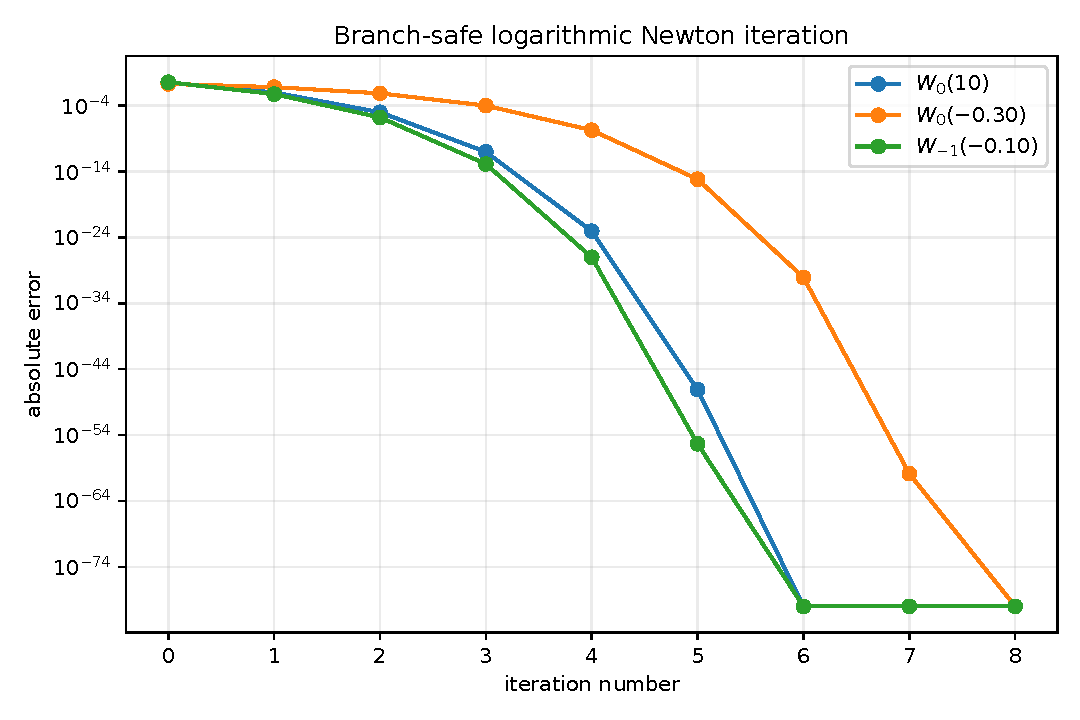
\includegraphics[width=.78\textwidth]{logarithmic_newton_convergence.pdf}
\caption{Monotone, eventually quadratic convergence of
\eqref{eq:lognewton} in three different branch regimes.}
\label{fig:lognewton}
\end{figure}

\subsection{A practical branch-aware algorithm}

For ordinary floating-point work, the following strategy is robust.

\begin{algorithm}[Real Lambert \(W\)]\label{alg:realW}
Given a real \(x\) and branch \(k\in\{0,-1\}\):
\begin{enumerate}
\item Reject inputs outside the branch domain.  Return \(-1\) exactly at
\(x=-1/\EulerE\), and return \(0\) for \(W_0(0)\).
\item If \(1+\EulerE x\) is tiny, evaluate the signed Puiseux series
\eqref{eq:puiseux-series}.
\item If \(k=0\) and \(|x|\) is small, use the Maclaurin series or a Pade
approximant.
\item If \(k=0\) and \(x\) is large, use
\eqref{eq:asymW0explicit} as a start.  If \(k=-1\) and \(x\) is close to
zero, use \eqref{eq:asymWmexplicit}.
\item Otherwise use a guaranteed start from \eqref{eq:globalstarts}.
\item Apply logarithmic Newton or Halley until the logarithmic residual and
the change in \(w\) are both below the requested tolerance.
\end{enumerate}
\end{algorithm}

If the input \(x<0\) is so small that it underflows, store
\(\lambda=\log(-x)\) instead.  Formula \eqref{eq:lognewton} then becomes
\begin{equation}\label{eq:loginput-newton}
       N_\lambda(w)
       =\frac{w}{1+w}\left(1+\lambda-\log(-w)\right),
\end{equation}
which never needs \(x\) itself.

\begin{literaturenote}
The 2022 paper by Lajos L\H{o}czi~\cite{loczi2022} in the supplied archive
develops guaranteed-precision versions of logarithmic Newton iteration, including
piecewise starting values and explicit error estimates over the full real
domains.  The paper by Iacono and Boyd~\cite{iacono2017} constructs global analytic
approximations and iteration-based refinements for \(W_0\).  Howard's Schr\"oder-series work~\cite{howard2025} studies higher-order
root-solving expansions.  The
present article emphasizes a shorter set of starts for which monotone
convergence can be proved directly by \cref{thm:lognewton-order}.
\end{literaturenote}

\subsection{Which approximation should be used?}

\begin{center}
\begin{tabularx}{.96\textwidth}{@{}lXl@{}}
\toprule
Regime & Recommended representation & Natural small parameter\\
\midrule
\(W_0\), \(x\approx0\) &
Maclaurin series or Pade approximant & \(x\)\\
Either branch, \(x\approx-1/\EulerE\) &
signed Puiseux series & \(p=\pm\sqrt{2(1+\EulerE x)}\)\\
\(W_0\), \(x\gg1\) &
logarithmic asymptotic series & \((\log\log x)/\log x\)\\
\(W_{-1}\), \(x\to0^-\) &
logarithmic asymptotic series & \(\log\eta/\eta\)\\
Moderate \(x\), high accuracy &
logarithmic Newton or Halley & current residual\\
Certified value &
monotone bracket plus residual bound & bracket width\\
\bottomrule
\end{tabularx}
\end{center}

There is no single best formula.  A high-quality implementation is a
carefully organized collection of mathematically equivalent formulas, each
used where it is well conditioned.


\section{Solving transcendental equations}\label{sec:equations}

The main skill is to isolate an expression of the form
\[
       Y\EulerE^Y=Z.
\]
Branch selection is then decided by the allowable range of the original
unknown, not by algebra alone.

\subsection{A linear term plus a logarithm}

\begin{theorem}\label{thm:axblogx}
Let \(a,b,c\in\RealNumbers\), with \(ab\neq0\), and seek \(x>0\) satisfying
\[
       ax+b\log x=c.
\]
Every real solution is
\begin{equation}\label{eq:axblogx}
       x=\frac ba\,
       W_k\left(\frac ab\EulerE^{c/b}\right),
\end{equation}
where a real branch is chosen so that the right side is positive.
\end{theorem}

\begin{proof}
Rearrange and exponentiate:
\[
       x=\EulerE^{c/b}\EulerE^{-(a/b)x}.
\]
Therefore
\[
       \frac abx\exp\left(\frac abx\right)
       =\frac ab\EulerE^{c/b}.
\]
Apply a real branch of \(W\), then multiply by \(b/a\).
Every reversible step preserves all positive solutions.
\end{proof}

Two important special cases are
\[
       x+\log x=c
       \quad\Longrightarrow\quad
       x=W_0(\EulerE^c),
\]
and
\begin{equation}\label{eq:xminuslogx}
       x-\log x=c
       \quad\Longrightarrow\quad
       x=-W_k(-\EulerE^{-c}).
\end{equation}
For \(c>1\), \eqref{eq:xminuslogx} has two positive solutions:
\(-W_0(-\EulerE^{-c})\in(0,1)\) and
\(-W_{-1}(-\EulerE^{-c})\in(1,\infty)\).  At \(c=1\), they coalesce at
\(x=1\).  This is exactly the two-branch geometry of
\cref{eq:vminuslogv}.

\subsection{A power times an exponential}

\begin{theorem}\label{thm:xpowerexp}
Let \(p\neq0\), \(q\neq0\), and suppose a consistent real \(p\)-th root of
\(A\) has been selected.  Solutions of
\[
       x^p\EulerE^{qx}=A
\]
that are compatible with that root are
\begin{equation}\label{eq:xpowerexp}
       x=\frac pq
       W_k\left(\frac qp A^{1/p}\right).
\end{equation}
\end{theorem}

\begin{proof}
Taking the selected \(p\)-th root gives
\(x\EulerE^{(q/p)x}=A^{1/p}\).  Multiplication by \(q/p\) produces the defining
Lambert equation.  Conversely, substitution verifies every value in
\eqref{eq:xpowerexp}.
\end{proof}

When \(p\) is even, taking a real root can introduce two signs.  Each sign
must be treated separately, and each resulting Lambert argument may itself
admit two real branches.

\begin{remark}[Endpoint-safe integer-power inverse package]
For \(m\in\NaturalNumbers\setminus\{0\}\), \(A>0\), and \(\beta>0\), the project sets
\[
 S_{m,A,\beta}(t)=At^m\EulerE^{-\beta t},
 \qquad
 P_{m,A,\beta}=A\left(\frac m\beta\EulerE^{-1}\right)^m
\]
and defines principal and lower Lambert phases \(\lambda_0\) and
\(\lambda_{-1}\).  Their exact endpoint-inclusive images are
\[
 \lambda_0\bigl([0,P_{m,A,\beta}]\bigr)
   =\left[0,\frac m\beta\right],
 \qquad
 \lambda_{-1}\bigl((0,P_{m,A,\beta}]\bigr)
   =\left[\frac m\beta,\infty\right].
\]
These are \path{principalPowerExponentialPhase_image_Icc} and
\path{lowerPowerExponentialPhase_image_Ioc}.  The theorems
\path{principalPowerExponentialPhase_invOn} and
\path{lowerPowerExponentialPhase_invOn} further say that each phase and
\(S_{m,A,\beta}\) are two-sided setwise inverses on the corresponding
displayed interval pair.  All four declarations are in
\path{PowerExponentialLambertInverse.lean}.  Thus this is a branch-explicit,
endpoint-safe integer-power specialization of \cref{thm:xpowerexp}, without
making an arbitrary-real-power root claim.

The normalized Lambert argument is continuous by
\path{powerExponentialLambertArgument_continuous}; the full phase statements
are \path{principalPowerExponentialPhase_continuousOn_Icc} on
\([0,P_{m,A,\beta}]\) and
\path{lowerPowerExponentialPhase_continuousOn_Ioc} on
\((0,P_{m,A,\beta}]\).  Moreover, if
\(0<x\leq P_{m,A,\beta}\) and \(\lambda\geq0\), then the exact equivalence
\[
 S_{m,A,\beta}(\lambda)=x
 \quad\Longleftrightarrow\quad
 \lambda=\lambda_0(x)\ \text{or}\ \lambda=\lambda_{-1}(x)
\]
is \path{powerExponentialSaddle_eq_iff_eq_principal_or_eq_lower}.  Strictly
inside the value interval the alternatives are distinct, by
\path{principalPowerExponentialPhase_ne_lowerPowerExponentialPhase}.  The
nonnegativity restriction is essential when even \(m\) permits additional
negative roots.

One further differentiation is formalized in
\path{PowerExponentialLambertCurvature.lean}.  For either
\(k\in\{0,-1\}\) and every \(0<x<P_{m,A,\beta}\), it gives
\begin{equation}\label{eq:power-exponential-phase-second-derivative}
 \lambda_k''(x)
 =\frac{\lambda_k(x)
   \left[m-\bigl(m-\beta\lambda_k(x)\bigr)^2\right]}
 {x^2\bigl(m-\beta\lambda_k(x)\bigr)^3}.
\end{equation}
The derivative witnesses are
\path{deriv_principalPowerExponentialPhase_hasDerivAt} and
\path{deriv_lowerPowerExponentialPhase_hasDerivAt}; the corresponding exact
formulas are \path{deriv_deriv_principalPowerExponentialPhase} and
\path{deriv_deriv_lowerPowerExponentialPhase}.  This generic module is
deliberately formula-only.  The sign and zero classifications at
\(\beta\lambda_0=m-\sqrt{m}\) and
\(\beta\lambda_{-1}=m+\sqrt{m}\), and the resulting generic strict-shape
theorems, are not yet packaged as Lean declarations.

The current zero-endpoint asymptotic package is exactly
\path{PowerExponentialLambertAsymptotics.lean}.  It proves
\path{principalPowerExponentialPhase_isEquivalent_rpow}, namely
\[
 \lambda_0(x)\sim\left(\frac{x}{A}\right)^{1/m}
 \qquad (x\downarrow0),
\]
and \path{tendsto_lowerPowerExponentialPhase_nhdsGT_zero_atTop}, namely
\(\lambda_{-1}(x)\to+\infty\).  For the intrinsic variable
\[
 \varepsilon(x)=\frac{\beta}{m}
   \left(\frac{x}{A}\right)^{1/m},
\]
\path{lowerPowerExponentialPhase_sub_intrinsicMain_tendsto_zero} gives only
the two-term statement
\[
 \lambda_{-1}(x)+\frac{m}{\beta}
 \bigl(\log\varepsilon(x)-\log|\log\varepsilon(x)|\bigr)
 \longrightarrow 0.
\]
No cleaned normalization in \(L=\log(A/x)\), nor a full generic asymptotic
series, is claimed by that module.

At \((m,A,\beta)=(1,1,\log2)\), the profile is
\(t2^{-t}\), its peak is \(\EulerE^{-1}/\log2\), and the principal specialization
is \path{fabiusPrincipalLambertPhase}.  The exact two-root equivalence and
strict interior distinctness become
\path{fabiusSaddle_eq_iff_eq_principal_or_eq_lower} and
\path{fabiusPrincipalLambertPhase_ne_fabiusLambertPhase}; continuity on the
closed principal and positive endpoint-inclusive lower value intervals is
\path{fabiusPrincipalLambertPhase_continuousOn_Icc} and
\path{fabiusLambertPhase_continuousOn_Ioc}.  Finally,
\path{fabiusPrincipalLambertPhase_isEquivalent_id} states that the principal
Fabius phase is asymptotic to \(x\) at zero, while
\path{lowerPowerExponentialPhase_one_one_log_two} in
\path{PowerExponentialLambertFabius}\texttt{.lean} identifies the lower generic phase
exactly with the Fabius lower-Lambert phase.

The separate specialization
\path{PowerExponentialLambertFabiusCurvature.lean} packages the complete
classical curvature geometry.  Put
\[
 L=\log2,\qquad P=\frac{\EulerE^{-1}}L,
 \qquad x_*=\frac{2\EulerE^{-2}}L.
\]
The definition \path{fabiusLambertInflectionInput} is \(x_*\),
\path{fabiusLambertInflectionInput_mem_Ioo} proves \(0<x_*<P\), and
\path{fabiusLambertPhase_inflectionInput} gives
\(\lambda_{-1}(x_*)=2/L\).  On \(0<x<P\),
\path{deriv_deriv_fabiusLambertPhase} states
\begin{equation}\label{eq:fabius-lower-phase-second-derivative}
 \lambda_{-1}''(x)
 =\frac{L\lambda_{-1}(x)^2\bigl(2-L\lambda_{-1}(x)\bigr)}
 {x^2\bigl(1-L\lambda_{-1}(x)\bigr)^3}.
\end{equation}
The declarations \path{deriv_deriv_fabiusLambertPhase_pos_iff},
\path{deriv_deriv_fabiusLambertPhase_neg_iff}, and
\path{deriv_deriv_fabiusLambertPhase_eq_zero_iff} say respectively that its
sign is positive for \(x<x_*\), negative for \(x_*<x\), and zero exactly at
\(x=x_*\); the named zero is
\path{deriv_deriv_fabiusLambertPhase_inflectionInput}.  Consequently
\path{strictConvexOn_fabiusLambertPhase_left} gives strict convexity on
\((0,x_*]\), while \path{strictConcaveOn_fabiusLambertPhase_right} gives
strict concavity on \([x_*,P]\).

The principal specialization is global to the left of the peak, not merely
restricted to positive profile inputs.  The bridge
\path{fabiusPrincipalLambertPhase_eq_principalLambertW} is
\[
 \lambda_0(x)=-\frac1L\Wz(-Lx).
\]
The declarations \path{fabiusPrincipalLambertPhase_continuousOn_Iic},
\path{fabiusPrincipalLambertPhase_hasDerivAt}, and
\path{deriv_fabiusPrincipalLambertPhase} give continuity on
\((-\infty,P]\) and first-order calculus on \((-\infty,P)\).
The derivative witness
\path{deriv_fabiusPrincipalLambertPhase_hasDerivAt} and exact formula
\path{deriv_deriv_fabiusPrincipalLambertPhase} give, for \(x<P\),
\begin{equation}\label{eq:fabius-principal-phase-second-derivative}
 \lambda_0''(x)
 =L\frac{\EulerE^{-2\Wz(-Lx)}\bigl(\Wz(-Lx)+2\bigr)}
          {\bigl(\Wz(-Lx)+1\bigr)^3}>0.
\end{equation}
Strict positivity is
\path{deriv_deriv_fabiusPrincipalLambertPhase_pos}, the regular value
\(\lambda_0''(0)=2L\) is
\path{deriv_deriv_fabiusPrincipalLambertPhase_zero}, and
\path{strictConvexOn_fabiusPrincipalLambertPhase} proves strict convexity on
the whole closed half-line \((-\infty,P]\).
\end{remark}

\subsection{An exponential equal to an affine function}

\begin{theorem}\label{thm:exp-affine}
Let \(\alpha\beta\neq0\).  Every solution of
\begin{equation}\label{eq:exp-affine}
       \EulerE^{\alpha x}=\beta x+\gamma
\end{equation}
is
\begin{equation}\label{eq:exp-affine-sol}
 \boxed{\displaystyle
 x=-\frac{\gamma}{\beta}
   -\frac1\alpha
 W_k\left(
  -\frac{\alpha}{\beta}
  \EulerE^{-\alpha\gamma/\beta}
 \right).}
\end{equation}
Real solutions correspond exactly to real branches available at the
displayed argument.
\end{theorem}

\begin{proof}
Set \(y=\beta x+\gamma\), so \(x=(y-\gamma)/\beta\).  Equation
\eqref{eq:exp-affine} becomes
\[
       \EulerE^{\alpha(y-\gamma)/\beta}=y.
\]
Multiplying by \(\exp(-\alpha y/\beta)\) and then by
\(-\alpha/\beta\) gives
\[
 \left(-\frac{\alpha y}{\beta}\right)
 \exp\left(-\frac{\alpha y}{\beta}\right)
 =
 -\frac{\alpha}{\beta}\EulerE^{-\alpha\gamma/\beta}.
\]
Apply \(W_k\), solve for \(y\), and then for \(x\).
\end{proof}

\begin{example}
The equation \(\EulerE^x=3x\) has argument \(-1/3\in(-1/\EulerE,0)\), so it has
two positive solutions:
\[
       x=-W_0(-1/3),\qquad x=-W_{-1}(-1/3).
\]
The two intersections of an exponential and a line are precisely the two
real Lambert branches.
\end{example}

\subsection{The equation \texorpdfstring{\(x^x=A\)}{x to the x equals A}}

\begin{theorem}[All positive solutions of \(x^x=A\)]\label{thm:xtox}
Let \(A>0\).  Positive solutions of \(x^x=A\) are
\begin{equation}\label{eq:xtox}
       x=\exp(W_k(\log A)).
\end{equation}
Their number is:
\begin{itemize}
\item one if \(A>1\);
\item one if \(A=1\), namely \(x=1\);
\item two if \(\EulerE^{-1/\EulerE}<A<1\);
\item one double minimum solution if \(A=\EulerE^{-1/\EulerE}\), namely
\(x=\EulerE^{-1}\);
\item none if \(0<A<\EulerE^{-1/\EulerE}\).
\end{itemize}
\end{theorem}

\begin{proof}
Put \(y=\log x\), so \(x=\EulerE^y\).  Taking logarithms of \(x^x=A\) gives
\[
       y\EulerE^y=\log A.
\]
Thus \(y=W_k(\log A)\), proving \eqref{eq:xtox}.  If \(\log A>0\), only
\(W_0\) is real.  If \(-1/\EulerE<\log A<0\), both \(W_0\) and \(W_{-1}\)
are real.  At \(\log A=-1/\EulerE\), they meet.  Below that value no real branch
exists.

For a direct calculus check, the derivative of
\(\log(x^x)=x\log x\) is \(1+\log x\), so \(x^x\) has its positive minimum
at \(x=\EulerE^{-1}\), with value \(\EulerE^{-1/\EulerE}\).
\end{proof}

\subsection{Fixed points of exponentiation}

A positive fixed point of
\[
       y=x^y
\]
satisfies
\begin{equation}\label{eq:power-tower-candidate}
       y=-\frac{W_k(-\log x)}{\log x}
       \qquad(x\neq1).
\end{equation}

\begin{proof}
Taking logarithms gives \(\log y=y\log x\).  Set
\(z=-y\log x\).  Then
\[
       z\EulerE^z=(-y\log x)\EulerE^{-y\log x}
             =(-y\log x)\frac1y
             =-\log x.
\]
Thus \(z=W_k(-\log x)\), which gives
\eqref{eq:power-tower-candidate}.
\end{proof}

For \(0<x<1\), the argument \(-\log x\) is positive and there is one positive
fixed point.  For \(1<x<\EulerE^{1/\EulerE}\), the argument lies in
\((-1/\EulerE,0)\), so there are two positive fixed points.  At
\(x=\EulerE^{1/\EulerE}\), they merge at \(y=\EulerE\).  This statement concerns
solutions of the fixed-point equation; convergence of the iterated power
tower is a separate dynamical question.

\subsection{A Planck-type maximization problem}

\begin{theorem}\label{thm:planckmax}
Let \(n>1\).  The function
\[
       F_n(x)=\frac{x^n}{\EulerE^x-1},\qquad x>0,
\]
has a unique critical point, which is its global maximum, at
\begin{equation}\label{eq:planckmax}
       x_n=n+W_0(-n\EulerE^{-n}).
\end{equation}
The second real branch gives
\[
       n+W_{-1}(-n\EulerE^{-n})=0,
\]
the boundary point rather than an interior maximum.
\end{theorem}

\begin{proof}
Logarithmic differentiation gives
\[
 \frac{F_n'(x)}{F_n(x)}
 =\frac nx-\frac{\EulerE^x}{\EulerE^x-1}.
\]
A critical point satisfies
\[
       n(\EulerE^x-1)=x\EulerE^x,
\]
or
\[
       (n-x)\EulerE^x=n.
\]
Put \(y=x-n\).  Then
\[
       y\EulerE^y=-n\EulerE^{-n},
\]
so \(x=n+W_k(-n\EulerE^{-n})\).  Since \(-n\leq-1\),
\cref{cor:inverse} gives
\(W_{-1}(-n\EulerE^{-n})=-n\), hence the boundary value \(x=0\).
The principal value lies in \((-1,0)\), so
\(x_n\in(n-1,n)\).

Finally \(F_n(x)\to0\) both as \(x\downarrow0\) (because \(n>1\)) and as
\(x\to\infty\).  The critical-point equation has only the one interior
solution just found, so that solution is the global maximum.
\end{proof}

\section{Applications}\label{sec:applications}

The point of a special function is not merely to rename an equation.  A
closed form exposes parameter dependence, branch multiplicity, asymptotic
regimes, and reliable initial values for computation.

\subsection{Michaelis--Menten substrate depletion}

Consider
\begin{equation}\label{eq:mm-ode}
       \frac{\Differential S}{\Differential t}
       =-\frac{V_{\max}S}{K_M+S},
       \qquad S(0)=S_0>0.
\end{equation}

\begin{theorem}\label{thm:mm}
The solution is
\begin{equation}\label{eq:mm-solution}
 S(t)=K_M W_0\left(
 \frac{S_0}{K_M}
 \exp\left[
 \frac{S_0}{K_M}-\frac{V_{\max}t}{K_M}
 \right]\right).
\end{equation}
\end{theorem}

\begin{proof}
Separate variables:
\[
       \left(1+\frac{K_M}{S}\right)\Differential S=-V_{\max}\Differential t.
\]
Integration and the initial condition give
\[
       S+K_M\log S
       =S_0+K_M\log S_0-V_{\max}t.
\]
Put \(y=S/K_M\) and \(y_0=S_0/K_M\).  Constants involving
\(\log K_M\) cancel, leaving
\[
       y+\log y=y_0+\log y_0-\frac{V_{\max}t}{K_M}.
\]
Exponentiation gives
\[
       y\EulerE^y
       =y_0\exp\left(y_0-\frac{V_{\max}t}{K_M}\right).
\]
The right side is positive, so the only real branch is \(W_0\), proving
\eqref{eq:mm-solution}.
\end{proof}

The archive paper by Goli\v{c}nik~\cite{golicnik2012} develops this and
related biochemical kinetic examples in detail.  Formula \eqref{eq:mm-solution} makes it possible to
differentiate with respect to parameters without repeatedly solving an
implicit equation.

\subsection{A diode with a series resistor}

Let \(I_S>0\) be the saturation current, \(R_S>0\) the series resistance,
and \(nV_T>0\) the thermal-voltage scale.  The Shockley law and the circuit
voltage relation are
\[
       I=I_S\left(\EulerE^{V_D/(nV_T)}-1\right),
       \qquad V=V_D+IR_S.
\]

\begin{theorem}\label{thm:diode}
The current is
\begin{equation}\label{eq:diode}
 I=
 \frac{nV_T}{R_S}
 W_0\left(
 \frac{R_SI_S}{nV_T}
 \exp\left[\frac{V+R_SI_S}{nV_T}\right]\right)-I_S.
\end{equation}
\end{theorem}

\begin{proof}
Let \(Y=I+I_S\).  Substitution of \(V_D=V-IR_S\) gives
\[
 Y=I_S\exp\left(\frac{V-R_S(Y-I_S)}{nV_T}\right).
\]
Therefore
\[
 Y\exp\left(\frac{R_SY}{nV_T}\right)
 =
 I_S\exp\left(\frac{V+R_SI_S}{nV_T}\right).
\]
Multiplication by \(R_S/(nV_T)\) produces a positive Lambert argument, so
\(W_0\) is the unique real branch.  Solving for \(I=Y-I_S\) gives
\eqref{eq:diode}.
\end{proof}

This branch-explicit form underlies the transistor and diode analyses in
Banwell's paper~\cite{banwell2000}.

\subsection{Characteristic exponents of a delay equation}

Consider
\begin{equation}\label{eq:dde}
       y'(t)=a\,y(t-\tau),\qquad \tau>0.
\end{equation}

\begin{theorem}\label{thm:dde}
Exponential modes \(y(t)=\EulerE^{\lambda t}\) have exponents
\begin{equation}\label{eq:dde-spectrum}
       \lambda_k=\frac1\tau W_k(a\tau),
       \qquad k\in\IntegerNumbers.
\end{equation}
\end{theorem}

\begin{proof}
Substitution gives
\[
       \lambda\EulerE^{\lambda t}
       =a\EulerE^{\lambda(t-\tau)},
\]
so \(\lambda=a\EulerE^{-\lambda\tau}\).  Hence
\[
       (\lambda\tau)\EulerE^{\lambda\tau}=a\tau,
\]
and \eqref{eq:dde-spectrum} follows.
\end{proof}

Here the infinitely many complex branches are not optional decoration:
they form the characteristic spectrum.  If
\(-1/\EulerE<a\tau<0\), the two real branches give two real characteristic
exponents in addition to the complex ones.

\subsection{The final-size equation of an epidemic model}

A common normalized SIR final-size equation is
\begin{equation}\label{eq:sir}
       \log\frac{s_\infty}{s_0}
       =-R_0(1-s_\infty),
\end{equation}
where \(R_0>0\) and \(0<s_\infty\leq s_0\leq1\).

\begin{theorem}\label{thm:sir}
Assume \(R_0>0\).  Every positive algebraic solution is
\begin{equation}\label{eq:sir-sol}
       s_\infty
       =-\frac1{R_0}
       W_k(-R_0s_0\EulerE^{-R_0}).
\end{equation}
The physically admissible branch must also satisfy
\(s_\infty\leq s_0\) and the assumptions under which
\eqref{eq:sir} was derived.
\end{theorem}

\begin{proof}
Exponentiating \eqref{eq:sir} gives
\[
       s_\infty=s_0\EulerE^{-R_0}\EulerE^{R_0s_\infty}.
\]
Thus
\[
 (-R_0s_\infty)\EulerE^{-R_0s_\infty}
 =-R_0s_0\EulerE^{-R_0},
\]
which proves \eqref{eq:sir-sol}.
\end{proof}

When two real branches are available, one may be a mathematically valid but
physically inadmissible root.  For example, if \(s_0=1\) and \(R_0>1\),
the identity
\[
       W_{-1}(-R_0\EulerE^{-R_0})=-R_0
\]
gives \(s_\infty=1\), the no-outbreak root, while \(W_0\) gives the smaller
nontrivial root.  Initial conditions and model interpretation decide which
one is relevant.

\subsection{Inverting the prime-number scale}

The rough relation
\[
       n\approx\frac{x}{\log x}
\]
arises when inverting the prime number theorem.  For \(n\geq\EulerE\), solving
the equality exactly and selecting its large solution gives
\begin{equation}\label{eq:primeinverse}
       x=-nW_{-1}(-1/n).
\end{equation}

\begin{proof}
Put \(y=\log x\), so \(x=\EulerE^y\).  The equation
\(x/\log x=n\) becomes
\[
       \frac{\EulerE^y}{y}=n,
\]
or
\[
       (-y)\EulerE^{-y}=-\frac1n.
\]
The large solution has \(y>1\), so \(-y<-1\), which selects \(W_{-1}\):
\(y=-W_{-1}(-1/n)\).  Exponentiating and using
\(\EulerE^{-W(z)}=W(z)/z\) gives
\(x=-nW_{-1}(-1/n)\).
\end{proof}

The principal branch would give a small root near \(x=1\), not the
large-\(x\) inverse relevant to primes.  Formula
\eqref{eq:asymWmexplicit} immediately yields
\[
 -nW_{-1}(-1/n)
 =n\left(\log n+\log\log n
 +\frac{\log\log n}{\log n}+\cdots\right),
\]
illustrating why the nonprincipal branch naturally enters prime asymptotics.
The archive paper by Visser develops this viewpoint for bounds on the
\(n\)-th prime.


\section{Series in a logarithmic argument}\label{sec:omega-series}

For positive arguments it is sometimes better to expand the Wright omega
function
\[
       \omega(t)=W_0(\EulerE^t)
\]
than to expand \(W_0(x)\) directly.  Its defining equation
\[
       \omega+\log\omega=t
\]
has no exponentially large quantity.

\begin{theorem}[Expansion centered at \(x=\EulerE\)]\label{thm:omega-e-series}
Let \(h=\log x-1\).  For \(x>0\) sufficiently close to \(\EulerE\),
\begin{align}
 W_0(x)
 ={}&1+\frac h2+\frac{h^2}{16}
 -\frac{h^3}{192}-\frac{h^4}{3072}
 +\frac{13h^5}{61440}
 +\BigO(h^6).\label{eq:omega-e-series}
\end{align}
\end{theorem}

\begin{proof}
Write \(\omega=1+s\) and \(t=1+h\).  The defining equation becomes
\[
       h=s+\log(1+s)
        =2s-\frac12s^2+\frac13s^3-\frac14s^4+\cdots.
\]
The derivative of the right side at \(s=0\) is \(2\neq0\), so it has an
analytic local inverse.  Substitute
\(s=c_1h+c_2h^2+\cdots\) and compare coefficients.  Successive comparison
gives
\[
 c_1=\frac12,\quad c_2=\frac1{16},\quad
 c_3=-\frac1{192},\quad c_4=-\frac1{3072},\quad
 c_5=\frac{13}{61440},
\]
which proves \eqref{eq:omega-e-series}.
\end{proof}

This representation, discussed in the Schroeder-series material in the
archive, is useful when an application supplies \(\log x\) directly.  Its
nonprincipal real analogue is not an ordinary Taylor series at the common
endpoint: if
\[
       \nu(\eta)=-W_{-1}(-\EulerE^{-\eta}),
\]
then \(\nu-\log\nu=\eta\) and the derivative with respect to \(\nu\)
vanishes at \((\eta,\nu)=(1,1)\).  The correct local expansion is therefore
the signed square-root series \eqref{eq:tseries}, not a Taylor series.  This
is another manifestation of the branch-point asymmetry.

\section{A brief guide to the complex branches}\label{sec:complex}

A complete construction of the Riemann surface belongs to complex analysis,
but the main ideas follow directly from the defining map.

\subsection{Local branches and the critical value}

The complex derivative of \(f(w)=w\EulerE^w\) is
\[
       f'(w)=\EulerE^w(1+w).
\]
Thus \(w=-1\) is the only finite critical point, and its critical value is
\(-1/\EulerE\).  At every other preimage \(w_*\), the complex inverse function
theorem gives a unique analytic local branch through \(w_*\).  Near
\(-1/\EulerE\), the same calculation as in \cref{sec:branchpoint} gives the
complex square-root coordinate
\[
       p=\sqrt{2(1+\EulerE z)}.
\]

At \(z=0\), the principal branch is regular and satisfies \(W_0(0)=0\).
The other branches escape to complex infinity as \(z\to0\), creating
logarithmic branching.

\subsection{Indexing and the all-branch asymptotic expansion}

For nonzero \(z\), choose a determination of \(\PrincipalLogarithm z\) and define
\[
       L_{1,k}=\PrincipalLogarithm z+2\pi\ImaginaryUnit k,\qquad
       L_{2,k}=\PrincipalLogarithm L_{1,k}.
\]
For large \(\AbsoluteValue{k}\), a solution is close to
\(L_{1,k}-L_{2,k}\).  The standard indexing \(W_k\) is chosen so that
\begin{equation}\label{eq:complex-leading}
       W_k(z)=L_{1,k}-L_{2,k}+\LittleO(1)
       \qquad(\AbsoluteValue{k}\to\infty),
\end{equation}
with consistent continuation away from branch cuts.

\begin{theorem}[Complex all-branch expansion]\label{thm:complex-asym}
Whenever \(\AbsoluteValue{L_{1,k}}\to\infty\) while the logarithms are chosen
consistently,
\begin{equation}\label{eq:complex-asym}
 W_k(z)\sim L_{1,k}-L_{2,k}
 +\sum_{n=1}^{\infty}
 \frac{\mathcal P_n(L_{2,k})}{L_{1,k}^n},
\end{equation}
with the same Stirling polynomials \(\mathcal P_n\) as in
\eqref{eq:Pn-asym}.
\end{theorem}

\begin{proof}
The complex equation is
\[
       W+\PrincipalLogarithm W=L_{1,k}.
\]
Set \(W=L_{1,k}-L_{2,k}+v\).  On a neighborhood where the logarithms are
consistent, exactly the algebra of \cref{thm:fullasym} gives
\[
       \tau=1-\EulerE^{-v}+\sigma v,\qquad
       \sigma=1/L_{1,k},\quad \tau=L_{2,k}/L_{1,k}.
\]
The Lagrange-inversion calculation and coefficient identity are algebraic
and remain valid over \(\ComplexNumbers\).  This proves
\eqref{eq:complex-asym}.
\end{proof}

This proof also shows that, for sufficiently large \(\AbsoluteValue{k}\), there is a
solution near \(L_{1,k}-L_{2,k}\): the implicit function theorem solves for
\(v\) when \(\sigma\) and \(\tau\) are small.  Hence a nonzero complex
argument has infinitely many Lambert values.

\subsection{Derivative and conjugation}

Every regular complex branch satisfies
\[
       W_k'(z)=\frac{W_k(z)}{z[1+W_k(z)]}.
\]
For a positive real \(x\), complex conjugation preserves
\(w\EulerE^w=x\).  Consistency with the asymptotic indexing gives
\[
       W_{-k}(x)=\overline{W_k(x)}.
\]
Thus nonreal values occur in conjugate pairs.

\begin{literaturenote}
Under the standard DLMF convention, \(W_0\) is analytic on
\(\ComplexNumbers\setminus(-\infty,-1/\EulerE]\); the other branches are organized
with cuts associated with the negative real axis and the logarithmic point
at zero.  Exact boundary labels require care because approaching a cut from
above or below can change the branch index.  The foundational paper of
Corless et al. and DLMF Section 4.13 give the complete sheet structure and
the standard conventions.
\end{literaturenote}

\section{What the supplied archive contributes}\label{sec:archive}

The archive is not treated as a collection of interchangeable authorities.
The foundational and reference sources establish notation and standard
formulas; later papers contribute targeted approximations, bounds,
algorithms, and applications.  The following map records how the material
was used.

\begin{longtable}{@{}>{\raggedright\arraybackslash}p{.29\textwidth}>{\raggedright\arraybackslash}p{.65\textwidth}@{}}
\toprule
Source in the archive & Main contribution to this article\\
\midrule
\endhead
Corless, Gonnet, Hare, Jeffrey, and Knuth (1996)~\cite{corless1996} &
Modern branch notation; Maclaurin, branch-point, and all-branch asymptotic
expansions; symbolic integration and numerical evaluation.  This is the
foundational modern reference.\\
\addlinespace
NIST DLMF, Section 4.13~\cite{dlmf} &
Canonical definitions, branch domains, coefficient conventions, asymptotic
formula, and the principal-branch integral representations proved in
\cref{sec:integralreps}.\\
\addlinespace
Barry et al. (2000)~\cite{barry2000} &
Piecewise analytic approximations for both real branches, with special care
at endpoints and with formulas designed as iteration starts.\\
\addlinespace
Banwell (2000)~\cite{banwell2000} &
Use of \(W_0\) to obtain explicit current--voltage formulas in diode and
bipolar-transistor circuits; see \cref{thm:diode}.\\
\addlinespace
Goli\v{c}nik (2012)~\cite{golicnik2012} &
Closed forms in biochemical kinetics, including integrated
Michaelis--Menten equations; see \cref{thm:mm}.\\
\addlinespace
Chatzigeorgiou (2013)~\cite{chatzigeorgiou2013} &
Elementary bounds for \(W_{-1}(-\EulerE^{-1-u})\).  A self-contained proof and
a midpoint error estimate appear in
\cref{thm:chatzbound,cor:Wm-midpoint}.\\
\addlinespace
Corcino, Corcino, and Mez\H{o} (2019)~\cite{corcino2019} &
Regular, associated, and Euler continued fractions.  The elementary Euler
fraction and its complete partial-sum proof appear in
\cref{thm:eulerW}.\\
\addlinespace
Iacono and Boyd (2017)~\cite{iacono2017} &
Global analytic approximations and iterative refinements for the principal
real branch, as well as approximation-based inequalities.\\
\addlinespace
L\H{o}czi (2022)~\cite{loczi2022} &
Guaranteed and arbitrary-precision evaluation on the full real domains,
especially logarithmic Newton recursions and explicit error control.\\
\addlinespace
Howard (2025) and the accompanying manuscript~\cite{howard2025} &
Schroeder-type and transformed series, including expansions in
\(\log x\), branch-point series, and comparisons of approximation regimes;
see \cref{sec:omega-series}.\\
\addlinespace
Lehtonen (2016)~\cite{lehtonen2016} &
A survey of ecological and evolutionary models whose implicit equations are
naturally inverted by Lambert \(W\).\\
\addlinespace
Visser (2018)~\cite{visser2018} &
Use of \(W_{-1}\) in explicit approximations and bounds for the \(n\)-th
prime; see \cref{eq:primeinverse}.\\
\addlinespace
ProductLog notebook and expository PDF/TXT files &
Computer-algebra notation, numerical cross-checks, and a broad inventory of
identities.  These were used as navigational aids rather than as primary
proof sources.\\
\bottomrule
\end{longtable}

Published maximum-error claims for fitted approximations depend on their
stated domains and numerical searches.  Rather than reproduce every fitted
constant, this article concentrates on formulas whose correctness and error
behavior can be proved directly: Taylor and Puiseux remainders, asymptotic
orders, two-sided bounds, residual certificates, and monotone Newton
iteration.  The supplied Python program independently checks representative
numerical behavior at high precision.

\section{Summary and a branch-safe workflow}\label{sec:summary}

The Lambert function is best understood not as one mysterious formula but as
a family of inverse maps.  The real-variable theory can be organized around
five decisions.

\begin{enumerate}[label=\textbf{Step \arabic*.},leftmargin=*]
\item \textbf{Count the real solutions before choosing a symbol.}
For \(-1/\EulerE<x<0\), there are two values.  The value in \((-1,0)\) is
\(W_0(x)\); the value in \(( -\infty,-1)\) is \(W_{-1}(x)\).

\item \textbf{Use the coordinate adapted to the endpoint.}
Near \(x=0\), use the Maclaurin series for \(W_0\).  Near the common branch
point, use the signed square-root coordinate
\(p=\pm\sqrt{2(1+\EulerE x)}\).  At the unbounded ends, use logarithmic
coordinates.

\item \textbf{Keep branch qualifications in inverse identities.}
The equation \(W(w\EulerE^w)=w\) is true only on the inverse interval belonging
to the selected branch.  This is exactly analogous to the restricted ranges
used for inverse trigonometric functions.

\item \textbf{For numerical work, combine an approximation with a
correction and a certificate.}
The branch-aware starts of \cref{thm:globalstarts}, logarithmic Newton
iteration, and the residual bounds of \cref{thm:residual} form a complete
real-variable procedure.

\item \textbf{Expect most algebraic identities to be branch-independent,
but most inequalities to be branch-dependent.}
The derivative, antiderivative, contour, and asymptotic calculations begin
from \(w\EulerE^w=x\) and therefore apply on every regular branch.  Monotonicity,
curvature, signs, and bounds depend on the range of the selected inverse.
\end{enumerate}

The two real branches are more symmetric than is sometimes suggested.
They share the same branch point, signed Puiseux series, logarithmic
asymptotic coefficient polynomials, inverse-function calculus, and monotone
logarithmic Newton map.  Their essential differences are global: \(W_0\) is
increasing and concave on its real domain, whereas \(W_{-1}\) is decreasing,
changes curvature once, and has a logarithmic singularity at zero.  The exact
pairing formulas of \cref{sec:pairing} make this balance particularly clear.

\section{Complements from the parallel treatments}\label{sec:complements}

The three parallel treatments merged into this volume derived the same core
theory --- branches, derivatives, Maclaurin and Puiseux series, asymptotic
polynomials, bounds, and Newton iteration --- with identical constants
throughout.  This section preserves their layers that the spine above does
not contain.  Attributions name the source package; the four-way concordance
is in \cref{app:concordance}.

\subsection{Power towers and iterated exponentials}

The fixed-point equation of the infinite tower
\(t_1=a\), \(t_{n+1}=a^{t_n}\) was solved in
\cref{sec:equations}; the monograph treatment settles \emph{convergence}
completely.

\begin{theorem}[Exact real power-tower interval]\label{cmp:thm:powertower}
For \(a>0\), the sequence of finite towers converges if and only if
\begin{equation}\label{cmp:eq:tower-interval}
 \EulerE^{-\EulerE}\le a\le\EulerE^{1/\EulerE},
\end{equation}
and throughout this interval its limit is
\(h=-W_0(-\log a)/\log a\) (with \(h=1\) at \(a=1\)).  For
\(1<a<\EulerE^{1/\EulerE}\), the second real branch \(W_{-1}\) gives another positive
solution of \(h=a^h\), which is repelling and is not the limit of the finite
towers.
\end{theorem}

\begin{proof}[Proof (monograph treatment)]
At a fixed point of \(g(x)=a^x\), \(g'(h)=h\log a=\log h\), so local
attraction requires \(1/\EulerE<h<\EulerE\); mapping the endpoints through
\(a=h^{1/h}\) produces \eqref{cmp:eq:tower-interval}.  For
\(1<a\le\EulerE^{1/\EulerE}\), \(h^{1/h}\) increases on \([1,\EulerE]\), so there is a
unique fixed point \(h\in[1,\EulerE]\), and since \(a\le h\) and \(g\) is
increasing with \(g([a,h])\subseteq[a,h]\), the towers increase to \(h\)
(including the neutral endpoint \(a=\EulerE^{1/\EulerE}\)).  For
\(\EulerE^{-\EulerE}\le a<1\), \(g\) is decreasing: the odd and even subsequences
are monotone with limits \(p\le h\le q\) forming a two-cycle
\(p=g(q)\), \(q=g(p)\).  Writing \(u=-\log p\), \(v=-\log q\), a nontrivial
two-cycle forces \(A:=-\log a=u\EulerE^v=v\EulerE^u\), hence, with \(r=u/v>1\),
\[
 A=\frac{r\log r}{r-1}\,r^{1/(r-1)},
\]
whose logarithm is strictly increasing in \(\log r\) (this reduces to
\(2\sinh(s/2)>s\)) with infimum \(1\); so \(A>\EulerE\), contradicting
\(A\le\EulerE\).  Hence \(p=q=h\), including the neutral endpoint
\(a=\EulerE^{-\EulerE}\).  Outside the interval no convergence occurs: for
\(a>\EulerE^{1/\EulerE}\) there is no fixed point, and for \(0<a<\EulerE^{-\EulerE}\) the
unique fixed point has \(\AbsoluteValue{g'(h)}>1\) and the injectivity of \(g\)
prevents the iterates from reaching it exactly.  The \(W_{-1}\) fixed point
\(H>\EulerE\) has \(g'(H)=\log H>1\).
\end{proof}

The companion equation \(x^y=y^x\) (fourth treatment): for positive
\(x\ne1\), it is equivalent to \((\log y)/y=(\log x)/x=:a\), so
\begin{equation}\label{cmp:eq:xyyx}
 y=-\frac1aW_k(-a),
\end{equation}
one branch reproducing \(y=x\) and, for \(0<a<1/\EulerE\), the other giving the
nontrivial partner (e.g.\ \(x=2\), \(y=4\)); the branches merge at
\(x=y=\EulerE\).

\subsection{Fixed-point, Schr\"oder, and inverse-Taylor methods}

Two evaluation methods complement the monotone Newton theory of
\cref{sec:numerics}.

\begin{proposition}[Logarithmic fixed-point iteration]
\label{cmp:prop:fixed-point}
The iteration \(w_{n+1}=\log(x/w_n)\) has fixed points exactly at the
nonzero branch values, with multiplier \(-1/W\) there.  It is locally
attracting exactly when \(\AbsoluteValue W>1\).  Thus the principal iteration attracts
only for \(x>\EulerE\), while the lower one attracts throughout
\(-1/\EulerE<x<0\).  Contraction fails at \(W_0(\EulerE)=1\) and at the branch point.
Where the iteration converges, its rate is only linear.
\end{proposition}

\begin{theorem}[Inverse-Taylor (Schr\"oder-type) corrections; monograph
treatment]\label{cmp:thm:inverse-taylor}
Let \(y\ne-1\) approximate a branch value, \(z_0=y\EulerE^y\), and
\(\Delta=x-z_0\).  Then
\begin{equation}\label{cmp:eq:schroeder}
 W(x)=y+\frac{\EulerE^{-y}}{1+y}\Delta
 -\frac{\EulerE^{-2y}(y+2)}{2(1+y)^3}\Delta^2
 +\frac{\EulerE^{-3y}(2y^2+8y+9)}{6(1+y)^5}\Delta^3
 +\BigO(\Delta^4),
\end{equation}
the coefficients being \(W^{(j)}(z_0)/j!\) from
\cref{thm:higherder}.  The linear truncation is exactly Newton's method for
\(w\EulerE^w=x\); truncation after \(\Delta^m\) turns an error
\(\varepsilon=y-W(x)\) into \(\BigO(\varepsilon^{m+1})\).  The quadratic
truncation costs little more than Newton and gives third-order local
accuracy; the powers of \((1+y)^{-1}\) warn against poor seeds near the
branch point.
\end{theorem}

Convenient global seeds for one or two corrections (monograph treatment):
\(y_0=\log(1+x)\) for \(W_0\), \(x>0\) (an upper bound by
\cref{thm:W0positivebounds}); \(y_0=x\) for \(W_0\) on \((-1/\EulerE,0)\);
\(y_0=-T-\log T\) with \(T=\log(1/(-x))\) for \(W_{-1}\); and the Puiseux
or logarithmic expansions at the ends.

\subsection{Structural identities and the branch-exchange involution}

The fourth treatment records several exact structures worth keeping
explicit.

\begin{itemize}
\item\textbf{Branch-exchange involution.}  For \(0<t\le1\),
\(\sigma(t)=-W_{-1}(-t\EulerE^{-t})\ge1\) satisfies
\(t\EulerE^{-t}=\sigma(t)\EulerE^{-\sigma(t)}\), and
\(s\mapsto-W_0(-s\EulerE^{-s})\) inverts it: the two real branches encode the
two inverse sides of the unimodal map \(q\mapsto q\EulerE^{-q}\).  (The exact
pair parametrization of \cref{sec:pairing} is the same involution in the
gap coordinate \(\Delta\).)
\item\textbf{Scaling.}  If \(w=W_k(x)\) and \(n\in\NaturalNumbers\), then
\[
 (nw)\EulerE^{nw}=\frac{nx^n}{w^{\,n-1}},
 \qquad\text{so}\qquad
 nW_k(x)=W_\ell\!\left(\frac{nx^n}{W_k(x)^{n-1}}\right)
\]
on the branch containing the value; similarly for complex \(\alpha\) with
consistent powers.
\item\textbf{Fixed points of \(W\).}  \(W_k(z)=z\) forces \(z\EulerE^z=z\),
i.e.\ \(z=0\) or \(z=2\pi\ImaginaryUnit n\); on the real principal branch the only
fixed point is \(0\).
\item\textbf{Unwinding.}  The frequently written identity
\(W_k(z)=\PrincipalLogarithm z-\PrincipalLogarithm W_k(z)+2\pi\ImaginaryUnit m\) carries a mandatory integer \(m\)
recording the logarithm discrepancy; on the real branches with absolute
values, \(W+\log\AbsoluteValue W=\log\AbsoluteValue x\) holds unambiguously.
\item\textbf{Closed Puiseux coefficients.}  Writing the branch-point
relation as \(u=q\,u/G(u)\) with
\(G(u)=u\sqrt{2\bigl(1+(u-1)\EulerE^u\bigr)/u^2}\), Lagrange inversion gives
the coefficients of the unified series \(S\) of \cref{thm:puiseux} in
closed form,
\begin{equation}\label{cmp:eq:puiseux-lagrange}
 a_n=\frac1n\,[t^{n-1}]\left(\frac t{G(t)}\right)^{\!n}.
\end{equation}
\item\textbf{Monodromy.}  Circling once around \(-1/\EulerE\) changes
\(p=\sqrt{2(1+\EulerE z)}\) to \(-p\) and interchanges the two local sheets ---
on the real side, exactly \(W_0\leftrightarrow W_{-1}\) (third treatment).
\end{itemize}

\subsection{A transcendence consequence}

\begin{theorem}[Fourth treatment]\label{cmp:thm:transcendence}
If \(z\ne0\) is algebraic, every value \(W_k(z)\) is transcendental.
\end{theorem}

\begin{proof}
If \(w=W_k(z)\) were algebraic (and nonzero, since \(z\ne0\)), then
Lindemann--Weierstrass makes \(\EulerE^w\) transcendental, contradicting
\(\EulerE^w=z/w\) algebraic.
\end{proof}

In particular the omega constant \(\Omega=W_0(1)\) is transcendental.
Values at transcendental arguments may still be algebraic --- e.g.\
\(W_0(\EulerE)=1\) and every manufactured value \(W_k(a\EulerE^a)=a\).

\subsection{A practitioner's toolkit}

Three habits from the third treatment simplify calculations in which \(W\)
appears inside a larger model.

\begin{itemize}
\item\textbf{Parameter sensitivity.}  If
\(w(\theta)=W_k(q(\theta))\) on a fixed branch, then
\[
 \nabla_\theta w=\frac{w}{q(1+w)}\,\nabla_\theta q
\]
away from \(q=0\), \(w=-1\) (with the limiting value
\(w'=q'\) at a principal-branch zero): every parameter derivative inherits
the branch-point factor \((1+w)^{-1}\).
\item\textbf{Differentiate in \(w\), not in \(x\).}  For differentiable
\(H\),
\(\tfrac{\Differential}{\Differential x}H(W(x))=H'(W(x))\,\EulerE^{-W(x)}/(1+W(x))\); computing
\(\Differential H/\Differential w\) first usually avoids nested quotient rules.
\item\textbf{Parametrize by \(w\).}  The substitution \(x=w\EulerE^w\) traces
each real branch with no numerical inversion (\(w\ge-1\) for \(W_0\),
\(w\le-1\) for \(W_{-1}\)); a conjectured inequality
\(A(x)\le W_0(x)\le B(x)\) becomes the inverse-free statement
\(A(w\EulerE^w)\le w\le B(w\EulerE^w)\).
\end{itemize}

Floating-point hazards (monograph and fourth treatments): near the branch
point, never form \(1+\EulerE x\) by naive subtraction when \(x\) is given as
\(-1/\EulerE+h\) --- compute \(p=\sqrt{2\EulerE h}\) from \(h\) directly or use
fused operations; for inputs so extreme that \(x\) overflows or underflows,
carry \(\log\AbsoluteValue x\) and use the logarithmic Newton map
\eqref{eq:loginput-newton}; and prefer the residual
\(w+\log\AbsoluteValue w-\log\AbsoluteValue x\) to \(w\EulerE^w-x\) as a stopping test.

\subsection{Further worked applications}

\begin{itemize}
\item\textbf{Optimal patch residence (marginal value theorem).}  With gain
\(G(t)=A(1-\EulerE^{-bt})\) and travel time \(\tau\), the rate-maximizing
residence time solves \(\EulerE^{bt}=1+b(t+\tau)\), and with \(y=1+b(t+\tau)>1\),
\begin{equation}\label{cmp:eq:patch}
 t_*=\frac{-W_{-1}(-\EulerE^{-1-b\tau})-1-b\tau}{b}:
\end{equation}
the principal branch would give negative residence time --- a clean case
where omitting \(W_{-1}\) loses the only admissible solution
\cite{lehtonen2016}.
\item\textbf{Wien displacement.}  Maximizing \(x^5/(\EulerE^x-1)\) gives
\((5-x)\EulerE^x=5\), so \(x_*=5+W_0(-5\EulerE^{-5})\approx4.9651142317\); the
lower branch returns the boundary root \(x=0\) via
\(W_{-1}(-5\EulerE^{-5})=-5\).  (Compare \cref{thm:planckmax} with \(n=5\).)
\item\textbf{Fall time with linear drag.}  From
\(s(t)=v_\infty[t-(1-\EulerE^{-\gamma t})/\gamma]\) and
\(A=1+\gamma s/v_\infty\ge1\),
\(t=[A+W_0(-\EulerE^{-A})]/\gamma\); the lower branch gives the negative-time
root of the extended equation.
\item\textbf{Schwarzschild tortoise coordinate.}  Inverting
\(r_*=r+2M\log(r/2M-1)\) for \(r>2M\):
\begin{equation}\label{cmp:eq:tortoise}
 r=2M\left[1+W_0\!\bigl(\EulerE^{\,r_*/(2M)-1}\bigr)\right],
\end{equation}
with the Wright omega form avoiding overflow for large \(r_*\).
\item\textbf{Prime counting.}  From \(p_n>n\log n\), inverting
\(u\log u\) gives
\(\pi(x)<x/W_0(x)=\EulerE^{W_0(x)}\) for \(x\ge2\), and
\(\pi(x)\sim x/W_0(x)\) restates the prime number theorem; the \(n\)th-prime
scale inversion is \eqref{eq:primeinverse}.
\end{itemize}

Every application above reduces to one of three normal forms (fourth
treatment): \((ax+b)\EulerE^{cx+d}=r\), solved by \(W\) directly;
\(x+\log x=c\), natural for \(W_0\)/Wright omega; and \(x-\log x=c\), the
two-branch inversion of \cref{eq:vminuslogv}.  Recognizing the form matters
more than any single formula.

\subsection{Generalizations and open directions}

The \emph{\(r\)-Lambert function} solves \(w\EulerE^w+rw=z\)
\cite{mezobaricz2017}; it has
\(W_r'(z)=\bigl[\EulerE^{W_r}(1+W_r)+r\bigr]^{-1}\), and its branch points are
images of the critical points \(\EulerE^w(1+w)+r=0\), themselves expressible by
ordinary \(W\).  More generally, equations
\(\EulerE^x\prod_i(x-t_i)/\prod_j(x-s_j)=a\) define generalized Lambert
functions; the practical diagnostic is that ordinary \(W\) applies exactly
when all appearances of the unknown gather into a single affine factor times
the exponential of an affine factor (\cref{thm:exp-affine}), and otherwise a
genuine generalization is required.  Approachable further directions
collected by the fourth treatment: minimax rational approximations after
mapping each unbounded branch to a finite interval; interval arithmetic with
sharp enclosures at the square-root point; the interlacing of
continued-fraction poles with the branch cut; real-variable analogues of
branch monodromy in parameter-dependent models where two physical roots
merge; and comparisons of \(W\), Wright omega, and \(r\)-Lambert
formulations for stiff delay equations.

\section{Role in the Fabius--Rvachev corpus}\label{sec:corpus-role}

Within this repository the Lambert function is not an isolated special
function: the lower real branch \(W_{-1}\) is the canonical coordinate of
the endpoint theory of the Fabius--Rvachev system.  The left-endpoint
asymptotics of the geometric-uniform laws have leading scale
\(-\log^2(1/x)/(2\log a)\), and inverting the associated saddle equations
produces exactly the coordinate \(-W_{-1}(-c\,x)\) with base-dependent
normalization \(c\) --- the dyadic all-orders endpoint and inverse-endpoint
expansions, their periodic Gamma--zeta phases, and the general-base
transform-level theory live in the exponents-and-\(q\)-series volume
(Parts VI--VII) and in the inverse-endpoint volume of this draft corpus,
with the exact phase-locked interpolation algebra formalized in
\path{LambertPhaseLockedRichardson.lean}.  A new finite algebraic rewrite
tranche identifies the complete-homogeneous factors in those exact moments
with complete Bell polynomials.  The division-free identity
\path{bellComplete_completeHomogeneousBellInput} and its factorially
normalized form
\path{completeHomogeneousEvalOn_eq_factorialNormalize_completeBellPolynomial}
are proved in \path{CompleteHomogeneousBell.lean}; the input at index
\(k+1\) is \(k!\) times the \((k+1)\)-st power sum.  The specialization in
\path{LambertPhaseLockedBell.lean} takes the alphabet
\((\lambda+j)^{-1}\), \(0\leq j\leq r\):
\path{completeHomogeneousEvalOn_shiftedReciprocal_eq_bell} rewrites its
degree-\(n\) complete-homogeneous value, while
\path{sum_shiftedReciprocalLagrangeWeight_mul_invPow_card_add_eq_bell} and
\path{sum_shiftedReciprocalLagrangeWeight_mul_invPow_eq_bell} give the exact
Bell forms of the residual moments at exponents \(r+1+n\) and \(r+s\)
(\(s\geq1\)), respectively.  The direct normalized specialization is stated
for a field with rational-algebra structure, and the weighted moment forms
assume characteristic zero.  Within that setting field inversion is total,
so no positivity or nonzero-shift hypothesis is added.

On the analytic side, the downstream modules
\path{FabiusLambertPhaseLockedPullback.lean},
\path{CompleteHomogeneousAsymptotics.lean},
\path{LambertReciprocalAsymptotics.lean}, and
\path{FabiusLambertPhaseExtraction.lean} now combine the arbitrary-order
endpoint remainder with the growing reciprocal row: for every fixed row
order \(r\) and residual depth \(S\), the periodic estimator minus its first
\(S\) exact residuals differs from the periodic endpoint term by
\(\BigO(\lambda^{-r-1-S})\), and it converges to the corresponding periodic
value along every integer phase ray.  This is a finite Poincar\'e statement,
and the Bell conversion is likewise an exact finite rewrite.  Neither gives
convergence of an infinite residual series, a multiplicative relative-error
hierarchy, a derivative extractor, uniformity in growing row order or
residual depth, or the outstanding sign control for those extensions.  The
two-term inversion
\(\log(1/G^{-1}(y))=\sqrt{2L\log(1/y)}-\tfrac12\log\log(1/y)+\BigO(1)\)
proved there is precisely the leading behavior of \(-W_{-1}\) in the
logarithmic regime of \cref{sec:asymptotics}, and the fixed-point/cocycle
structure behind those expansions is the \(v-\log v=u\) geometry of
\cref{eq:vminuslogv}.  This volume supplies the function-level foundations
--- branches, expansions, bounds, and certified evaluation --- on which
those corpus layers stand.

\clearpage
\appendix

\section{A complete proof of Lagrange--Buer\-mann inversion}
\label{app:lagrange}

This appendix proves the coefficient theorem used in the Maclaurin and
asymptotic sections.  The proof is algebraic and therefore works for formal
power series; no question of numerical convergence is involved.

\subsection{Formal residues}

For a Laurent series \(A(t)=\sum_{j\in\IntegerNumbers}a_jt^j\), define
\[
       \ResidueOperator_{t=0} A(t)\Differential t=a_{-1}.
\]
Two elementary rules will be used.

\begin{lemma}[Derivative and substitution rules]\label{lem:formal-residue}
Let \(A(t)\) be a formal Laurent series.
\begin{enumerate}[label=\textup{(\roman*)}]
\item \(\ResidueOperator A'(t)\Differential t=0\).
\item If \(y=y(x)=c_1x+c_2x^2+\cdots\) with \(c_1\neq0\), then
\begin{equation}\label{eq:formal-change}
       \ResidueOperator_{x=0}A(y(x))y'(x)\Differential x
       =\ResidueOperator_{y=0}A(y)\Differential y.
\end{equation}
\end{enumerate}
\end{lemma}

\begin{proof}
For (i), the derivative of \(a_jt^j\) is \(ja_jt^{j-1}\).  A term in
\(t^{-1}\) could arise only from \(j=0\), but its coefficient is then zero.

For (ii), linearity reduces the proof to \(A(y)=y^m\).  If \(m\neq-1\),
then
\[
       y(x)^m y'(x)
       =\frac1{m+1}\frac{\Differential}{\Differential x}y(x)^{m+1},
\]
whose residue is zero by part (i); the residue of \(y^m\Differential y\) is also zero.
If \(m=-1\), write \(y(x)=c_1x[1+xB(x)]\).  Then
\[
       \frac{y'(x)}{y(x)}
       =\frac1x+\frac{\Differential}{\Differential x}\log[1+xB(x)],
\]
so its residue is \(1\), exactly the residue of \(\Differential y/y\).  This proves
the substitution rule term by term.
\end{proof}

\subsection{Proof of the inversion formula}

Suppose
\begin{equation}\label{eq:appendix-implicit}
       y=x\phi(y),\qquad \phi(0)\neq0.
\end{equation}
There is a unique formal solution \(y(x)=c_1x+c_2x^2+\cdots\): after
substituting the two series, the coefficient of \(x^n\) determines \(c_n\)
from the preceding coefficients, beginning with \(c_1=\phi(0)\).

Let \(H\) be a formal power series and \(n\geq1\).  Coefficient extraction
is a residue:
\begin{equation}\label{eq:coeff-residue}
       [x^n]H(y(x))
       =\ResidueOperator_{x=0}\frac{H(y(x))}{x^{n+1}}\Differential x.
\end{equation}
From \eqref{eq:appendix-implicit},
\[
       x=\frac{y}{\phi(y)},
       \qquad
       \Differential x=\frac{\phi(y)-y\phi'(y)}{\phi(y)^2}\Differential y.
\]
The substitution rule of \cref{lem:formal-residue} therefore changes
\eqref{eq:coeff-residue} into
\begin{align}
 [x^n]H(y(x))
 &=\ResidueOperator_{y=0}
 \left[
 \frac{H(y)\phi(y)^n}{y^{n+1}}
 -\frac{H(y)\phi(y)^{n-1}\phi'(y)}{y^n}
 \right]\Differential y.
 \label{eq:lagrange-mid}
\end{align}
Now differentiate
\[
       \frac{H(y)\phi(y)^n}{y^n}.
\]
Its residue is zero, so
\begin{align*}
 0={}&\ResidueOperator_{y=0}\left[
 \frac{H'(y)\phi(y)^n}{y^n}
 +n\frac{H(y)\phi(y)^{n-1}\phi'(y)}{y^n}
 -n\frac{H(y)\phi(y)^n}{y^{n+1}}
 \right]\Differential y.
\end{align*}
Rearranging and comparing with \eqref{eq:lagrange-mid} gives
\[
 [x^n]H(y(x))
 =\frac1n\ResidueOperator_{y=0}
       \frac{H'(y)\phi(y)^n}{y^n}\Differential y
 =\frac1n[y^{n-1}]H'(y)\phi(y)^n.
\]
This is \eqref{eq:lagrange}.  Taking \(H(y)=y^m\) gives
\[
 [x^n]y(x)^m
 =\frac{m}{n}[y^{n-m}]\phi(y)^n,
\]
which is \eqref{eq:lagrange-power}.  Thus every form of Lagrange inversion
used in the article has now been proved.

\section{Coefficient tables and exact recurrences}\label{app:coefficients}

The formulas in the main text are designed to generate coefficients, not
merely to list them.  The following tables are convenient for checking hand
calculations and computer implementations.

\subsection{Maclaurin coefficients}

Write
\[
       W_0(x)=\sum_{n\geq1}c_nx^n,
       \qquad c_n=\frac{(-n)^{n-1}}{n!}.
\]
The first ten coefficients are
\begin{center}
\begin{tabular}{@{}c r@{\qquad}c r@{}}
\toprule
\(n\)&\(c_n\)&\(n\)&\(c_n\)\\
\midrule
1&\(1\)&6&\(-54/5\)\\
2&\(-1\)&7&\(16807/720\)\\
3&\(3/2\)&8&\(-16384/315\)\\
4&\(-8/3\)&9&\(531441/4480\)\\
5&\(125/24\)&10&\(-156250/567\)\\
\bottomrule
\end{tabular}
\end{center}
The last entry is intentionally left in a moderately factored rational form;
the closed formula is usually more informative than a decimal expansion.

\subsection{Signed branch-point coefficients}

With \(p=\pm\sqrt{2(1+\EulerE x)}\), write
\[
       W=-1+\sum_{n\geq1}a_np^n.
\]
The first nine coefficients, generated by
\eqref{eq:brec}--\eqref{eq:arec}, are
\begin{center}
\begin{tabular}{@{}c r@{\qquad}c r@{}}
\toprule
\(n\)&\(a_n\)&\(n\)&\(a_n\)\\
\midrule
1&\(1\)&6&\(-221/8505\)\\
2&\(-1/3\)&7&\(680863/43545600\)\\
3&\(11/72\)&8&\(-1963/204120\)\\
4&\(-43/540\)&9&\(226287557/37623398400\)\\
5&\(769/17280\)&&\\
\bottomrule
\end{tabular}
\end{center}
The same table serves both branches; only the sign of \(p\) changes.

\subsection{Derivative polynomials}

The recurrence in \cref{thm:higherder} begins
\begin{align*}
 P_1(w)&=1,\\
 P_2(w)&=-(w+2),\\
 P_3(w)&=2w^2+8w+9,\\
 P_4(w)&=-(6w^3+36w^2+79w+64),\\
 P_5(w)&=24w^4+192w^3+622w^2+974w+625.
\end{align*}
Consequently
\[
 W_k^{(n)}(x)
 =\frac{\EulerE^{-nW_k(x)}P_n(W_k(x))}
       {[1+W_k(x)]^{2n-1}}.
\]
This form avoids differentiating an increasingly complicated quotient from
scratch.

\section{Numerical experiments and reproducibility}\label{app:numerics}

The archive accompanying this article contains
\texttt{numerical\_experiments.py}.  It uses
\texttt{mpmath} at 80 decimal digits to obtain reference values and then
implements, independently, the approximations proved in the article:

\begin{itemize}
\item the signed branch-point series for both real branches;
\item the logarithmic asymptotic expansion for \(W_0\) and \(W_{-1}\);
\item the three Pad\'e approximants of \cref{sec:rational};
\item the two-sided \(W_{-1}\) bounds;
\item the branch-safe logarithmic Newton iteration.
\end{itemize}

From the directory containing the source, run
\begin{lstlisting}[language=bash]
python3 numerical_experiments.py --output-dir figures
\end{lstlisting}
The required packages are \texttt{mpmath}, \texttt{numpy}, and
\texttt{matplotlib}; the script does not use network access.  Every plotting
function writes a vector PDF, so the figures remain sharp when enlarged.
The reference values and defining-equation residuals are also written to
\texttt{numerical\_values.txt}.

\lstinputlisting[
  language={},
  basicstyle=\ttfamily\footnotesize,
  breaklines=true,
  caption={High-precision reference values generated by the supplied script.}
]{numerical_values.txt}

The reference implementation is not used as a hidden proof.  Its purpose is
to detect transcription mistakes, illustrate the proved convergence orders,
and make every graph reproducible.  Analytic statements in the main text are
established independently of the plots.

\section{Problems with complete solutions}\label{app:problems}

These exercises review the main ideas without requiring complex analysis.

\subsection*{Problems}
\begin{enumerate}[label=\textbf{P\arabic*.},leftmargin=*]
\item Prove that the equation \(w\EulerE^w=-1/10\) has exactly two real
solutions, and locate each one in an interval of length \(1\).

\item Let \(a\geq-1\).  Prove \(W_0(a\EulerE^a)=a\).  Let \(a\leq-1\).
Prove \(W_{-1}(a\EulerE^a)=a\).  Explain why the branch restrictions cannot be
removed.

\item Solve \(x+2\log x=5\) for \(x>0\).

\item Evaluate
\(\displaystyle\int_{-1/\EulerE}^{0}W_{-1}(x)\Differential x\).

\item Show directly from the defining equation that
\[
       \frac{\Differential}{\Differential x}\EulerE^{W_0(x)}
       =\frac1{1+W_0(x)}
       \qquad(x>-1/\EulerE).
\]

\item For \(-1/\EulerE<x<0\), prove
\(W_0(x)+W_{-1}(x)<-2\) without differentiating either branch.

\item Determine the number of positive real solutions of \(x^x=A\) for
\(A>0\), and express them with the correct Lambert branches.

\item Derive the first three nonconstant terms in the expansion of
\(W_0(x)\) at \(x=0\) by substituting
\(W_0(x)=a_1x+a_2x^2+a_3x^3+\BigO(x^4)\) into the defining equation.

\item Let \(x>\EulerE\), \(L=\log x\).  Prove that
\(L-\log L<W_0(x)<L\).

\item Suppose an approximation \(w\) to a selected real Lambert value
satisfies \(w\neq0,-1\).  Derive one logarithmic Newton step without using
\(\EulerE^w\).
\end{enumerate}

\subsection*{Solutions}
\begin{enumerate}[label=\textbf{S\arabic*.},leftmargin=*]
\item Since \(-1/\EulerE<-1/10<0\), \cref{thm:realbranches} gives exactly two
solutions.  On \((-1,0)\),
\((-1)\EulerE^{-1}<-1/10<0\), so the principal solution lies in \((-1,0)\).
For the lower branch,
\[-4\EulerE^{-4}\approx-0.0733>-0.1,
  \qquad -3\EulerE^{-3}\approx-0.1494<-0.1.
\]
Because \(w\EulerE^w\) is decreasing on \(( -\infty,-1)\), the second solution
lies in \((-4,-3)\).

\item The map \(w\mapsto w\EulerE^w\) is one-to-one from \([-1,\infty)\) onto
\([-1/\EulerE,\infty)\), so its inverse there sends \(a\EulerE^a\) back to \(a\).
This is \(W_0\).  The same argument on \(( -\infty,-1]\), where the map is
one-to-one onto \([-1/\EulerE,0)\), gives the \(W_{-1}\) identity.  Without the
range restriction, an input in \((-1/\EulerE,0)\) has two preimages, so a single
inverse formula cannot select both.

\item Divide by \(2\): \(x/2+\log x=5/2\).  Exponentiation gives
\(x\EulerE^{x/2}=\EulerE^{5/2}\).  Hence
\[
       \frac{x}{2}\EulerE^{x/2}=\frac12\EulerE^{5/2},
       \qquad
       x=2W_0\left(\frac12\EulerE^{5/2}\right).
\]
The argument is positive, so only \(W_0\) is real.

\item By \eqref{eq:defintWm}, the answer is \(-3/\EulerE\).  Directly, put
\(w=W_{-1}(x)\).  Then \(w\) runs from \(-1\) to \(-\infty\), and
\[
 \int w\EulerE^w(1+w)\Differential w
 =\left[\EulerE^w(w^2-w+1)\right]_{-1}^{-\infty}
 =-\frac3\EulerE.
\]

\item Differentiate and use \eqref{eq:firstder}:
\[
 \frac{\Differential}{\Differential x}\EulerE^{W_0(x)}
 =\EulerE^{W_0(x)}W_0'(x)
 =\EulerE^{W_0(x)}\frac{\EulerE^{-W_0(x)}}{1+W_0(x)}.
\]
The factors cancel.

\item Let \(\Delta=W_0(x)-W_{-1}(x)>0\).  By
\eqref{eq:pair-sum}, the sum is
\(-\Delta\coth(\Delta/2)\).  Put \(y=\Delta/2\).  The function
\(y\cosh y-\sinh y\) has value \(0\) at \(0\) and positive derivative
\(y\sinh y\), so \(y\coth y>1\).  The sum is therefore less than \(-2\).

\item Put \(u=\log x\).  Then \(x^x=A\) becomes
\(u\EulerE^u=\log A\), so
\[
       x=\exp[W_k(\log A)].
\]
If \(A>1\), then \(\log A>0\) and there is one solution, from \(W_0\).
If \(A=1\), the positive solution is \(x=1\).  If
\(\EulerE^{-1/\EulerE}<A<1\), then \(-1/\EulerE<\log A<0\) and there are two
solutions, from \(W_0\) and \(W_{-1}\).  If
\(A=\EulerE^{-1/\EulerE}\), the two coalesce at \(x=\EulerE^{-1}\).  If
\(0<A<\EulerE^{-1/\EulerE}\), there is no positive real solution.

\item Expand \(\EulerE^W=1+W+W^2/2+\BigO(x^3)\).  Then
\[
 W\EulerE^W=W+W^2+\frac12W^3+\BigO(x^4).
\]
Substitution gives
\[
 a_1x+(a_2+a_1^2)x^2+
 (a_3+2a_1a_2+a_1^3/2)x^3+\BigO(x^4)=x.
\]
Thus \(a_1=1\), \(a_2=-1\), and \(a_3=3/2\).

\item Since \(L\EulerE^L=Lx>x\) and \(w\EulerE^w\) is increasing for
\(w>0\), one has \(W_0(x)<L\).  Put \(a=L-\log L\).  Then
\[
       a\EulerE^a=x\left(1-\frac{\log L}{L}\right)<x,
\]
so the same monotonicity gives \(a<W_0(x)\).

\item Apply Newton's method to
\(G(w)=w+\log|w|-\log|x|\).  Since \(G'(w)=1+1/w\),
\begin{align*}
 w^+&=w-\frac{w+\log|w|-\log|x|}{1+1/w}\\
 &=\frac{w}{1+w}\left(1+\log\left|\frac{x}{w}\right|\right).
\end{align*}
This is \eqref{eq:lognewton}.
\end{enumerate}

\section{Compact formula sheet}\label{app:formula-sheet}

\begin{longtable}{@{}p{.26\textwidth}p{.68\textwidth}@{}}
\toprule
Topic & Formula and branch condition\\
\midrule
\endhead
Definition & \(W_k(x)\EulerE^{W_k(x)}=x\).\\
\addlinespace
Real domains & \(W_0:[-1/\EulerE,\infty)\to[-1,\infty)\), increasing;
\(W_{-1}:[-1/\EulerE,0)\to(-\infty,-1]\), decreasing.\\
\addlinespace
Derivative & On \(W_0\) for \(x>-1/\EulerE\), and on \(W_{-1}\) for
\(-1/\EulerE<x<0\),
\(W_k'(x)=\EulerE^{-W_k(x)}/[1+W_k(x)]\).  When \(x\neq0\), this is also
\(W_k(x)/\{x[1+W_k(x)]\}\); separately, \(W_0'(0)=1\).\\
\addlinespace
Second derivative & On the same smooth domains,
\(W_k''(x)=-\EulerE^{-2W_k(x)}[W_k(x)+2]/[1+W_k(x)]^3\).  When
\(x\neq0\), this is also
\(-W_k(x)^2[W_k(x)+2]/\{x^2[1+W_k(x)]^3\}\); separately,
\(W_0''(0)=-2\).\\
\addlinespace
Antiderivative &
\(\int W_k(x)\Differential x=\EulerE^{W_k(x)}[W_k(x)^2-W_k(x)+1]+C\).\\
\addlinespace
Maclaurin &
\(W_0(x)=\sum_{n\geq1}(-n)^{n-1}x^n/n!\), \(|x|<1/\EulerE\).\\
\addlinespace
Branch point &
\(W_{0,-1}(x)=-1+p-p^2/3+11p^3/72-\cdots\),
\(p=\pm\sqrt{2(1+\EulerE x)}\).\\
\addlinespace
Large \(W_0\) &
\(W_0(x)=L_1-L_2+L_2/L_1+\cdots\),
\(L_1=\log x\), \(L_2=\log L_1\).\\
\addlinespace
Small-negative \(W_{-1}\) & Same coefficient formula with
\(L_1=\log(-x)<0\), \(L_2=\log[-L_1]\).\\
\addlinespace
Exact branch pair &
If \(\Delta=W_0-W_{-1}\), then
\(W_0=-\Delta/(\EulerE^\Delta-1)\) and
\(W_{-1}=-\Delta/(1-\EulerE^{-\Delta})\).\\
\addlinespace
Logarithmic Newton &
\(w^+=\dfrac{w}{1+w}\left(1+\log\left|x/w\right|\right)\).\\
\addlinespace
Residual certificate &
\(|w-W_k(x)|\leq|w\EulerE^w-x|/\min_I|\EulerE^t(1+t)|\), provided the interval
\(I\) between \(w\) and the root avoids \(-1\).\\
\bottomrule
\end{longtable}

\section{Lean formalization crosswalk}\label{app:lean-crosswalk}

The repository's Lean library carries a two-branch development of the real
Lambert function, and several of the foundational statements of this guide
are exact theorems there.  This appendix records the correspondence, in the
discipline of the other frontier volumes: a row names declarations, all in
namespace \lean{Fabius}, and a row is listed only when the Lean statement
has the displayed mathematical content.  Where the Lean statement is
weaker, more general, or differently normalized than the guide's, the
difference is stated.  Everything not listed here is unformalized.

The two branches are \decl{principalLambertW} (\(\Wz\), totalized, intended
domain \([-1/\EulerE,\infty)\); module \lean{PrincipalLambertW}) and
\decl{lowerLambertW} (\(\Wm\), intended domain \([-1/\EulerE,0)\); module
\lean{LowerLambertW}).  Both are defined as the logarithm of an inverse of
\(u\mapsto u\log u\) on the appropriate ray, so ``\(W(x)\)'' is a total
real function whose values off the intended domain are junk; every theorem
below carries the domain hypothesis explicitly.

The focused branch-pair and Bernoulli tranche is exhaustive at this checkpoint:
\lean{LambertWBranchPairing} has \(0+7\) public definitions/theorems,
\lean{LambertWGapBijection} has \(4+16\), and
\lean{LambertWBranchSymmetry} has \(0+9\), while
\lean{LambertWBranchGapBernoulli} has \(0+5\).  Their four-module union is
therefore four definitions and 37 theorems, 41 public declarations in all.
The preceding exact-radius checkpoint had the then-current census 903/11,447; the
complex value-completion theorem brought the next historical checkpoint to
903/11,448.  The later sibling
\path{GeometricUniformMomentPolynomial.lean} module has \(1+8\) public
definitions/theorems and raised the next historical census to 904/11,457.
Its companion \path{GeometricUniformMomentPolynomialBridge.lean} has the
exhaustive count \(0+1\) and raised the next historical census to 905/11,458.
Its sole
theorem,
\leansubtwo{geometricUniformMomentPolynomial_eval}{_eq_mgf_taylorCoefficient},
supplies the real-\(\lvert q\rvert<1\) actual-MGF normalization and makes
\nolinkurl{p7:eq:Pn-def} Exact in that regime.  It supplies no complex-q
infinite-product realization by itself.  The subsequent current \(1+3\)
\path{GeometricUniformComplexMomentProduct.lean} leaf consists of
\nolinkurl{geometricUniformComplexMomentProduct},
\nolinkurl{hasProdLocallyUniformly_geometricUniformComplexMomentProduct},
\nolinkurl{differentiable_geometricUniformComplexMomentProduct}, and
\leansubtwo{geometricUniformMomentPolynomial_eval}{_eq_complexMomentProduct_taylorCoefficient}.
For every complex \(\lVert q\rVert<1\), these give the actual locally uniform
product, prove complex differentiability on the whole plane, and identify its
normalized Taylor coefficient with the recursive polynomial.  This is a
complex analytic analogue, not a complex probability-moment extension of
\nolinkurl{p7:eq:Pn-def}, whose Exact status
remains restricted to real \(\lvert q\rvert<1\).  At this historical point the
canonical q-monograph compound \nolinkurl{thm:qF-moment-polynomial} remained
Partial because neither the global \texttt{RatFunc} identification nor its
pole-clearing polynomial continuation at roots was formalized.  The original
\(1+2\) complex surface raised the next
incoming-branch checkpoint to the historical 906/11,461, and in the merged
chronology it formed the historical 918/11,568 checkpoint; the subsequently
exposed differentiability theorem belongs only to the live census below.  The exhaustive
zero-definition/one-theorem \path{HalfQBinomialRootSimplicity.lean} leaf then
gave the merged-main 919/11,569 checkpoint.  Its
\nolinkurl{halfQBinomial_sum_rootMultiplicity_two_pow}, together with the
existing complete rational root classification, makes
\nolinkurl{cor:halfbase-root-locus} Exact.  No arbitrary-base or
arbitrary-field simplicity is claimed, and
\nolinkurl{cor:qbinom-inversion-law} remains Partial.  The subsequent
exhaustive \(1+2\)
\path{GeometricUniformExteriorComplexMomentGerm.lean} sibling consists of
\nolinkurl{geometricUniformExteriorComplexMomentGerm},
\nolinkurl{analyticAt_geometricUniformExteriorComplexMomentGerm}, and
\leansubtwo{geometricUniformMomentPolynomial_eval}{_eq_exteriorComplexMomentGerm_taylorCoefficient}.
For every complex \(q\) with \(1<\lVert q\rVert\), these define the actual
reciprocal germ, prove its analyticity at the origin, and identify its
normalized Taylor coefficient with the recursive polynomial.  No unit-circle
or global rational-function claim is made.  The exterior leaf raises the
census to 920/11,572.

The final exhaustive \(0+3\)
\path{GeometricUniformMomentPolynomialDegree.lean} sibling consists of
\nolinkurl{coeff_geometricUniformMomentPolynomial_choose_two},
\nolinkurl{coeff_geometricUniformMomentPolynomial_choose_two_sub_one}, and
\nolinkurl{geometricUniformMomentPolynomial_natDegree_eq}.  With
\(T_n=\binom n2\), these prove the top coefficient \(B_n(1)/n!\), the
subleading coefficient
\(-B_n(1)/n!+B_{n-1}(1)/(2(n-1)!)\) for \(n\geq2\), and degree \(T_n\) for
even \(n\) or \(n=1\), one less otherwise.  Here Lean's
\nolinkurl{bernoulli'} is \(B_n(1)=(-1)^nB_n\) under Mathlib's convention
\(B_1=-1/2\).  This makes \nolinkurl{p7:thm:Pn} and
\nolinkurl{prop:qF-P-degree-sharp} Exact.  At that checkpoint the global
\nolinkurl{thm:qF-moment-polynomial} was still Partial for the separate
\texttt{RatFunc}/root-continuation gap.  The sharp leaf raises the census to
the historical 921/11,575 checkpoint.  The exhaustive
\path{RvachevLaurentLeading.lean} \((1+6)\) sibling then gives 922/11,582 and
makes \nolinkurl{is:p2:thm:Laurent-leading} Exact.  The exhaustive
\path{FinitePrefixAppellRecovery.lean} \((11+17)\) sibling gives the
historical 923/11,610 checkpoint and makes
\nolinkurl{is:p2:thm:finite-prefix-expansion} and
\nolinkurl{is:p2:thm:exact-recovery} Exact as finite rational identities.
Retaining the unconditional public
\lean{complexQPochhammerInf_eq_qPochhammerInfIn} bridge gives the historical
semantic-union checkpoint 957/11,921.  Adding the residual-existence
certificate \lean{exists_eq_in_residual_interval} gives the current union
computed by \path{scripts/doc_audit.py} and pinned in
\path{docs/doc_audit_baseline.json}, with both documentation gap counts zero.
The q-Lucas manuscript result remains Partial: Lean proves
the evaluated primitive-root identity, not the polynomial congruence modulo
the cyclotomic polynomial.

The final exhaustive \(1+4\)
\path{GeometricUniformMomentRatFunc.lean} sibling consists of
\nolinkurl{geometricUniformMomentRatFunc},
\nolinkurl{qFactorial_mul_geometricUniformMomentRatFunc},
\nolinkurl{eval_geometricUniformMomentRatFunc_eq_complexMomentProduct_taylorCoefficient},
\nolinkurl{eval_geometricUniformMomentRatFunc_eq_exteriorComplexMomentGerm_taylorCoefficient},
and \nolinkurl{eval_geometricUniformMomentRatFunc_one}.  It packages one
\texttt{RatFunc} over the rationals, proves the global q-factorial clearing
identity, identifies that same rational function with both strict
off-unit-circle Taylor-coefficient regimes, and handles \(q=1\) through
\([n]_1!=n!\).  Together with the recursive polynomial leaf, this makes
\nolinkurl{thm:qF-moment-polynomial} Exact and gives the historical
924/11,615 checkpoint.  No analytic value, pole order, or divisor is asserted
at a genuine unit-root pole.  The later
\path{GeometricUniformMomentReciprocity.lean} sibling consists of one public
definition, \nolinkurl{geometricUniformComplexMomentGerm}, and five public
theorems:
\nolinkurl{geometricUniformComplexMomentGerm_of_norm_lt_one},
\nolinkurl{geometricUniformComplexMomentGerm_of_one_lt_norm},
\nolinkurl{analyticAt_geometricUniformComplexMomentGerm},
\nolinkurl{geometricUniformComplexMomentGerm_reciprocity}, and
\nolinkurl{geometricUniformComplexMomentGerm_moment_convolution}.  It identifies
the strict inner and exterior branches, proves analyticity at zero off the unit
circle, and proves for \(q\ne0\) and \(\lVert q\rVert\ne1\) the local germ
identity \(M_q(z)M_{q^{-1}}(-z)=1\) and its exact all-order binomial derivative
convolution.  Thus \nolinkurl{thm:qF-reciprocity} is Exact; no global pointwise
identity through genuine inner-product zeros is asserted.  The later
\nolinkurl{weightedSumDistribution_real_Ici_eq_rvachevUp_of_nonneg} and
\nolinkurl{integral_pow_weightedSumDistribution_eq_mul_intervalIntegral_rvachevUp}
theorems make \nolinkurl{prop:up-tail} and \nolinkurl{cor:up-moments} Exact.
The unrelated exhaustive (1+1)
\path{RvachevLegendreBiorthogonality.lean} leaf consists of
\nolinkurl{rvachevLegendreAnalysisKernel} and
\nolinkurl{rvachevLegendreBiorthogonality}; it closes the translated-kernel
definition and finite Legendre biorthogonality, but not the larger
Fourier--Bessel or projector claims.  These additions give the historical
925-module/11,619-declaration checkpoint.  Subsequent source-only
tranches, including the reciprocity sibling, give the historical reciprocity
checkpoint of 931 modules and 11,685 public declarations.  The subsequently
merged upstream \path{DyadicBoundaryIdentity.lean} and
\path{FinitePrefixThueMorseCollapse.lean} modules add two modules and ten
public declarations, making the historical dyadic/finite-prefix census 933
modules and 11,695 public declarations.  The incoming union adds one module
and fourteen public declarations: the new zero-definition/six-theorem
\path{ProuhetBaseTwoBridge.lean} module, one theorem added to
\path{DyadicBoundaryIdentity.lean}, and seven theorems added to
\path{ThueMorseNewmanSelfSimilarity.lean}.  That historical tranche reached
934 modules and 11,709 public declarations.  The frozen merge target now has
957 modules and 11,920 public declarations; retaining the unconditional
public \lean{complexQPochhammerInf_eq_qPochhammerInfIn} bridge gives the
historical semantic-union checkpoint 957/11,921, and the residual-existence
certificate is included in the current union computed by
\path{scripts/doc_audit.py} and pinned in
\path{docs/doc_audit_baseline.json}, with zero documentation gaps.  The rigorous q
forward ledger is 181 Exact / 79 Partial / 14 None / 8 interface rows, the relevant Dyadic
Gaussian--Thue--Morse chapter is 13/43/0/0, and its source concordance is
103 Lean-proved / 375 human-proved frontier / 60 non-applicable / 9 conjectures.
The q-Lucas row remains Partial because the Lean result is an evaluated
primitive-root identity, not the polynomial congruence modulo the cyclotomic
polynomial.

\begin{longtable}{@{}p{0.30\textwidth}p{0.42\textwidth}p{0.22\textwidth}@{}}
\toprule
Statement in this guide & Exact Lean declaration(s) & Remarks\\
\midrule
\endfirsthead
\toprule
Statement in this guide & Exact Lean declaration(s) & Remarks\\
\midrule
\endhead
\Cref{thm:realbranches}: \(\Wz\) is a strictly increasing bijection
\([-1/\EulerE,\infty)\to[-1,\infty)\), \(\Wm\) a strictly decreasing
bijection \([-1/\EulerE,0)\to(-\infty,-1]\), and every real solution of
\(w\EulerE^w=x\) is one of the two &
\decl{principalLambertW\_strictMonoOn},
\decl{principalLambertW\_image\_Ioi}, \decl{principalLambertW\_image\_Icc},
\decl{neg\_one\_le\_principalLambertW},
\decl{lowerLambertW\_strictAntiOn}, \decl{lowerLambertW\_image},
\decl{lowerLambertW\_le\_neg\_one},
\decl{eq\_principalLambertW\_or\_eq\_lowerLambertW} &
The last, in module \lean{LambertBranchDichotomy}, is the dichotomy:
\(w\EulerE^w=z\) forces \(w=\Wz(z)\) or \(w=\Wm(z)\).  The images are
stated for the open ray \((-1/\EulerE,\infty)\) and the interval
\([-1/\EulerE,0]\) on the principal side and the open interval
\((-1/\EulerE,0)\) on the lower side; the endpoint values are separate
lemmas.\\
\addlinespace
\Cref{cor:inverse}: \(\Wz(a\EulerE^a)=a\) for \(a\geq-1\) and
\(\Wm(a\EulerE^a)=a\) for \(a\leq-1\) &
\decl{principalLambertW\_unique},
\decl{lowerLambertW\_unique\_of\_mem\_Ico}; the defining equations
\(W(x)\EulerE^{W(x)}=x\) are \decl{principalLambertW\_mul\_exp} and
\decl{lowerLambertW\_mul\_exp\_of\_mem\_Ico} &
Stated as uniqueness: any \(w\geq-1\) with \(w\EulerE^w=z\) equals
\(\Wz(z)\), and dually for \(w\leq-1\).\\
\addlinespace
\Cref{thm:derivatives}, first and second derivatives &
\decl{deriv\_principalLambertW}, \decl{deriv\_deriv\_principalLambertW}
(module \lean{LambertWCurvature});
\decl{deriv\_lowerLambertW}, \decl{deriv\_deriv\_lowerLambertW} &
The principal-branch first derivative is in the form
\eqref{eq:firstder}, the lower-branch one in the form
\eqref{eq:firstder-x}; both second derivatives are in the exponential form
\eqref{eq:secondder-exp}.  \(\Wz'(0)=1\) is
\decl{principalLambertW\_isEquivalent\_zero}, stated as
\(\Wz(z)\sim z\) at \(0\).  Positivity of \(\Wz'\) is
\decl{deriv\_principalLambertW\_pos}.\\
\addlinespace
\Cref{thm:curvature}: \(\Wz\) strictly concave; \(\Wm\) strictly convex on
\((-1/\EulerE,-2/\EulerE^2)\), inflection at \(-2/\EulerE^2\), strictly
concave on \((-2/\EulerE^2,0)\) &
\decl{strictConcaveOn\_principalLambertW},
\decl{strictConvexOn\_lowerLambertW\_left},
\decl{strictConcaveOn\_lowerLambertW\_right},
\decl{deriv\_deriv\_lowerLambertW\_eq\_zero\_iff} &
Lean's concavity of \(\Wz\) is on the closed ray \([-1/\EulerE,\infty)\),
slightly more than stated here; the lower-branch pieces are on the closed
interval \([-1/\EulerE,-2/\EulerE^2]\) and the half-open
\([-2/\EulerE^2,0)\).  The inflection is stated as
\(\Wm''(x)=0\iff x=-2/\EulerE^2\) on the open domain.\\
\addlinespace
\Cref{thm:maclaurin}, \Cref{thm:cayley}: the Maclaurin coefficients
\((-n)^{n-1}/n!\) &
\decl{coeff\_lambertW} (module \lean{LambertWSeries}) &
A statement about the \emph{formal} series over \(\RationalNumbers\): the
compositional inverse of \(X\EulerE^{X}\) has \((n+1)\)-st coefficient
\((-(n+1))^n/(n+1)!\).  It is obtained from the library's
Lagrange--B\"urmann inversion (\Cref{thm:lagrange}), and carries no
statement about convergence, the radius \(1/\EulerE\), or the endpoint;
those remain unformalized.\\
\addlinespace
\Cref{thm:puiseux}, leading term: \(\Wz(x)+1\sim q\) and
\(\Wm(x)+1\sim-q\) as \(x\downarrow-1/\EulerE\), with
\(q=\sqrt{2(1+\EulerE x)}\) &
\decl{principalLambertW\_add\_one\_isEquivalent\_branchPoint},
\decl{lowerLambertW\_add\_one\_isEquivalent\_branchPoint} (module
\lean{LambertWBranchPointAsymptotics}); non-differentiability at the branch
point, \decl{principalLambertW\_not\_differentiableAt\_branchPoint} and
\decl{lowerLambertW\_not\_differentiableAt\_branchPoint} (module
\lean{LambertWBranchPointGeometry}) &
Only the leading square-root term is formal; the full signed Puiseux series
and its coefficients are not.\\
\addlinespace
\Cref{lem:logineq}: \(t/(1+t)\leq\log(1+t)\leq t\) for \(t>-1\) &
Mathlib: \nolinkurl{Real.log_le_sub_one_of_pos} and
\nolinkurl{Real.one_sub_inv_le_log_of_pos} &
Both halves are Mathlib lemmas (not repository declarations), stated at
\(1+t>0\); the strict upper form is
\nolinkurl{Real.log_lt_sub_one_of_pos}.\\
\addlinespace
\Cref{thm:W0positivebounds}: \(x/(1+x)\leq\Wz(x)\leq\log(1+x)\leq x\) for
\(x\geq0\), strict for \(x>0\) &
\decl{principalLambertW\_elementary\_bounds},
\decl{div\_one\_add\_le\_principalLambertW},
\decl{principalLambertW\_le\_log\_one\_add},
\decl{principalLambertW\_le\_self}, and the strict
\decl{div\_one\_add\_lt\_principalLambertW},
\decl{principalLambertW\_lt\_log\_one\_add} (module
\lean{LambertWElementaryBounds}) &
Proved from a single inequality with no Lambert content, valid for
\emph{every} real \(w\): \decl{exp\_le\_one\_add\_mul\_exp\_self},
\(\EulerE^w\leq1+w\EulerE^w\), strict for \(w\neq0\); the guide's
\(w=\Wz(x)\) is one instance, and \decl{le\_log\_one\_add\_mul\_exp} states
the upper bound for every real \(w\) in the form
\(w\leq\log(1+w\EulerE^w)\).\\
\addlinespace
\Cref{thm:Wmzerobounds}: for \(-1/\EulerE<x<0\) and
\(\eta=\log(1/(-x))\),
\(-\eta-\eta\log\eta/(\eta-1)\leq\Wm(x)<-\eta-\log\eta\) &
\decl{lowerLambertW\_near\_zero\_bounds}, with the halves
\decl{neg\_log\_sub\_div\_le\_lowerLambertW} and
\decl{lowerLambertW\_lt\_neg\_log\_sub} (module
\lean{LowerLambertW}) &
The mechanism is the bracket for the inverse of \(z-\log z\), stated with no
Lambert content for every \(y>1\) with \(y-\log y=\eta\):
\decl{SubLog.bracket\_of\_sub\_log\_eq}, from
\decl{SubLog.strictMonoOn\_sub\_log}.  The reduction
\(y=-\Wm(x)\), \(y-\log y=\eta\) is
\decl{neg\_lowerLambertW\_sub\_log\_eq}, and \(\eta>1\) on the whole domain is
\decl{one\_lt\_log\_one\_div\_neg}, so the denominator \(\eta-1\) is never a
side condition for the caller.\\
\addlinespace
\Cref{thm:higherder}: every derivative of either branch is
\(W^{(n)}=\EulerE^{-nW}P_n(W)/(1+W)^{2n-1}\) with
\(P_{n+1}=(1+w)P_n'-(nw+3n-1)P_n\) &
\decl{lambertDerivPoly}, \decl{lambertDerivPoly\_succ},
\decl{iteratedDeriv\_principalLambertW},
\decl{iteratedDeriv\_lowerLambertW} (module
\lean{LambertWHigherDerivatives}); the general engine is
\decl{AutonomousODE.iteratedDeriv\_eq\_comp} (module
\lean{AutonomousIteratedDeriv}) &
Lean's \(P_n\) is this guide's \(P_{n+1}\): the recurrence is stated as
\(P_{n+1}=(1+w)P_n'-((n+1)w+3n+2)P_n\) from \(P_0=1\), and the formula as
\(W^{(n+1)}=\EulerE^{-(n+1)W}P_n(W)/(1+W)^{2n+1}\), on the open domains
\((-1/\EulerE,\infty)\) and \((-1/\EulerE,0)\).  The engine is stated for an
arbitrary solution of an autonomous equation \(W'=\varphi\circ W\) on an open
set, with the derivative family as hypotheses, so it applies beyond Lambert's
function.\\
\addlinespace
\Cref{thm:antiderivatives}: \(\int W_k=\EulerE^{W_k}(W_k^2-W_k+1)
=x(W_k-1+1/W_k)\) and \(\int W_k/x=W_k+\tfrac12W_k^2\) &
\decl{hasDerivAt\_principalLambertW\_antiderivative},
\decl{hasDerivAt\_lowerLambertW\_antiderivative},
\decl{hasDerivAt\_principalLambertW\_add\_half\_sq},
\decl{hasDerivAt\_lowerLambertW\_add\_half\_sq} (module
\lean{LambertWAntiderivative}); the general forms
\decl{LambertAntiderivative.hasDerivAt\_exp\_mul\_sq\_sub\_add\_one},
\decl{LambertAntiderivative.hasDerivAt\_add\_half\_sq} and the two-form
identity \decl{LambertAntiderivative.exp\_mul\_sq\_sub\_add\_one\_eq} &
Stated as derivative facts (\(F'=W\), \(G'=W/x\)) on the open branch
domains, which is the content of the antiderivative statement.  The general
forms assume only \(W'=(\EulerE^{W}(1+W))^{-1}\) at the point, with
\(W\neq-1\), so they hold for any local inverse of \(w\mapsto w\EulerE^w\);
the \(x\)-form needs \(W\neq0\) and the \(W/x\) form needs \(x\neq0\), as in
the guide.\\
\addlinespace
\Cref{thm:W0logbounds}: for \(x>\EulerE\), \(L=\log x\),
\(L-\log L<\Wz(x)<L-\log(L-\log L)<L\) &
\decl{principalLambertW\_log\_bounds}, with the halves
\decl{log\_sub\_log\_log\_lt\_principalLambertW},
\decl{principalLambertW\_lt\_log\_sub\_log\_log\_sub\_log\_log},
\decl{principalLambertW\_lt\_log} (module \lean{LambertWLogBounds}); the
non-strict outer bracket for \(x\geq\EulerE\) is
\decl{principalLambertW\_log\_bracket} (module
\lean{PrincipalLambertWAtTop}) and the non-strict sharper upper bound
\decl{principalLambertW\_le\_log\_sub\_log\_log\_sub\_log\_log} &
Exact.  All from \(W+\log W=L\) (\decl{principalLambertW\_add\_log}) and
monotonicity of the logarithm; the equality \(\Wz(\EulerE)=1\) at the
endpoint is \decl{principalLambertW\_exp\_one}.\\
\addlinespace
\Cref{prop:addition}: \((a+b)\EulerE^{a+b}=xy(1/a+1/b)\) for Lambert
values \(a,b\neq0\) of \(x,y\), hence \(a+b=W_m(xy(1/a+1/b))\) on the branch
containing \(a+b\) &
\decl{mul\_exp\_add\_of\_mul\_exp} (the identity, for any reals satisfying
their defining equations), \decl{add\_eq\_principalLambertW\_of\_mul\_exp},
\decl{add\_eq\_lowerLambertW\_of\_mul\_exp},
\decl{principalLambertW\_add\_principalLambertW} (module
\lean{LambertWAdditionIdentity}) &
Exact.  The branch consequence is stated through the uniqueness theorems:
\(a+b\geq-1\) selects \(\Wz\), and \(a+b\leq-1\) with the product in
\([-1/\EulerE,0)\) selects \(\Wm\); for \(x,y>0\) the two principal values
add to the principal value, with no side condition.\\
\addlinespace
\Cref{thm:pairing}, forward direction: with \(\Delta=\Wz(x)-\Wm(x)>0\) on
\((-1/\EulerE,0)\), \(\Wz=-\Delta/(\EulerE^\Delta-1)\),
\(\Wm=-\Delta/(1-\EulerE^{-\Delta})
=-\Delta\EulerE^\Delta/(\EulerE^\Delta-1)\),
\(x=\Wz\EulerE^{\Wz}\) in the \(\Delta\)-form, and the \(t=\EulerE^\Delta\)
forms &
\decl{principalLambertW\_sub\_lowerLambertW\_pos},
\decl{lowerLambertW\_eq\_principalLambertW\_mul\_exp\_gap},
\decl{principalLambertW\_eq\_neg\_gap\_div},
\decl{lowerLambertW\_eq\_neg\_gap\_mul\_exp\_div},
\decl{lowerLambertW\_eq\_neg\_gap\_div\_one\_sub\_exp\_neg},
\decl{eq\_neg\_gap\_div\_mul\_exp},
\decl{principalLambertW\_lowerLambertW\_eq\_of\_exp\_gap} (module
\lean{LambertWBranchPairing}) &
Exact for the forward direction.  The whole computation is
\(\Wm=\Wz\EulerE^\Delta\) from dividing the two defining equations.\\
\addlinespace
\Cref{thm:pairing}, converse: every \(\Delta>0\) inserted into the formulas
produces one and only one \(x\in(-1/\EulerE,0)\), with the displayed values
equal to \(\Wz(x)\) and \(\Wm(x)\) &
\decl{gapPrincipal}, \decl{gapLower}, \decl{gapArg} (the three formulas as
functions of \(\Delta\)), \decl{branchGap} (the map
\(x\mapsto\Wz(x)-\Wm(x)\)); \decl{gapArg\_mem\_Ioo},
\decl{principalLambertW\_gapArg}, \decl{lowerLambertW\_gapArg},
\decl{branchGap\_gapArg}, \decl{gapArg\_branchGap}; the two directions
packaged as \decl{branchGap\_invOn} and \decl{branchGap\_bijOn}; and the
three \(t>1\) coordinate formulas are
\decl{principalLambertW\_gapArg\_log},
\decl{lowerLambertW\_gapArg\_log}, and \decl{gapArg\_log} (module
\lean{LambertWGapBijection}) &
Exact, and stated as a bijection: \(x\mapsto\Delta\) is a bijection from
\((-1/\EulerE,0)\) onto \((0,\infty)\) with the explicit inverse
\(\Delta\mapsto a(\Delta)\EulerE^{a(\Delta)}\), \(a(\Delta)=-\Delta/(\EulerE^\Delta-1)\).
The proof is uniqueness on each branch: \(b(\Delta)=a(\Delta)\EulerE^\Delta\)
equals \(a(\Delta)-\Delta\), so \(b\EulerE^b=a\EulerE^a\), and
\(-1<a<0\), \(b<-1\) are the tangent-line inequalities
\(\Delta<\EulerE^\Delta-1\) and \(\EulerE^\Delta(1-\Delta)<1\).\\
\addlinespace
\Cref{cor:pair-symmetric}: the exact quotient, sum, and product identities,
and \(\Wz(x)+\Wm(x)<-2\),
\(0<\Wz(x)\Wm(x)<1\) on \((-1/\EulerE,0)\) &
\decl{lowerLambertW\_div\_principalLambertW\_eq\_exp\_branchGap},
\decl{principalLambertW\_add\_lowerLambertW\_eq\_exp\_branchGap},
\decl{principalLambertW\_add\_lowerLambertW\_eq\_cosh\_div\_sinh\_branchGap},
\decl{principalLambertW\_mul\_lowerLambertW\_eq\_exp\_branchGap},
\decl{principalLambertW\_mul\_lowerLambertW\_eq\_sinh\_sq\_branchGap},
\decl{principalLambertW\_add\_lowerLambertW\_lt\_neg\_two},
\decl{principalLambertW\_mul\_lowerLambertW\_pos},
\decl{principalLambertW\_mul\_lowerLambertW\_lt\_one}, and
\decl{principalLambertW\_mul\_lowerLambertW\_mem\_Ioo} (module
\lean{LambertWBranchSymmetry}) &
Exact.  The exponential-rational sum and product forms strengthen the printed
hyperbolic identities, and the final theorem packages the two strict product
bounds.  The left endpoint is sharp: at \(x=-1/\EulerE\), both branches are
\(-1\), hence the sum is \(-2\) and the product is \(1\); the open hypotheses
are therefore essential.  The endpoint \(x=0\) remains excluded because the
lower real branch has no finite value there.\\
\addlinespace
\eqref{eq:bernoulli-gen}, with the standard removable-origin convention above,
and \eqref{eq:pair-Bernoulli-general}: the complex Bernoulli generating
identity and the compact paired series for \(0<\Delta<2\pi\) on
\(-1/\EulerE<x<0\), together with the exact convergence locus &
\decl{summable\_norm\_bernoulli\_mul\_pow\_div\_factorial},
\decl{summable\_bernoulli\_mul\_pow\_div\_factorial\_iff},
\decl{hasSum\_bernoulli\_mul\_pow\_div\_factorial},
\decl{hasSum\_bernoulli\_mul\_pow\_div\_factorial\_complex\_iff}, and
\decl{principalLambertW\_lowerLambertW\_eq\_bernoulliSeries} (module
\lean{LambertWBranchGapBernoulli}) &
{\footnotesize Exact for the complex generating identity, the compact real branch pair, and
the convergence locus.  The
first theorem proves absolute summability for every real
\(z\) with \(\lvert z\rvert<2\pi\); the second proves, for complex \(z\), that
the Bernoulli series is summable if and only if \(\lVert z\rVert<2\pi\), hence
it diverges on \(\lVert z\rVert=2\pi\) and throughout the exterior; the third
proves the actual all-index real sum \(z/(\exp z-1)\) when \(z\ne0\); the
fourth proves the complex \(\operatorname{HasSum}\) value
\(\lean{complexExpm1Div}(z)^{-1}\) if and only if
\(\lVert z\rVert<2\pi\); and the fifth specializes both real sums on the
strict common branch domain when the positive branch gap is below \(2\pi\).
At \(z=0\), the fourth theorem's target is the removable value \(1\); away
from zero it rewrites to the literal quotient.  This makes both displayed
identities in this row Exact under the stated convention, but claims no
equality with Lean's totalized quotient at zero.  The compiled radius proof
uses even Bernoulli--zeta coefficient bounds and a positive even subsequence;
it does not formalize the Guide's nearest-nonzero-zero explanation.  The
surrounding expanded displays and every Puiseux claim remain unpromoted.}\\
\addlinespace
\Cref{thm:W0negativebounds}: for \(-1/\EulerE<x<0\),
\(-1+\sqrt{1+\EulerE x}<\Wz(x)<-1+\sqrt{2(1+\EulerE x)}\) and \(\Wz(x)<x\) &
\decl{principalLambertW\_negative\_bounds}, with the halves
\decl{neg\_one\_add\_sqrt\_lt\_principalLambertW},
\decl{principalLambertW\_lt\_neg\_one\_add\_sqrt},
\decl{principalLambertW\_lt\_self\_of\_neg} (module
\lean{LambertWNegativeBounds}) &
Exact.  In the shifted variable \(s=\Wz+1\in(0,1)\) the two square-root bounds
are the exponential inequalities \(\EulerE^s>1+s\) and
\(\EulerE^s(1-s)<1-s^2/2\); the second is
\decl{exp\_mul\_one\_sub\_lt\_one\_sub\_half\_sq}, proved from its derivative
\(s(\EulerE^s-1)>0\), with no Lambert content.\\
\bottomrule
\end{longtable}

Not formalized, in the order they appear above: the moments of
\Cref{sec:integrals}, the local Taylor expansion, convergence of the
Maclaurin series, the full Puiseux and
logarithmic asymptotic expansions, the remaining bounds of
\Cref{sec:bounds} (the two-sided \(W_{-1}\) bound of
\Cref{thm:chatzbound}), and everything from
\Cref{sec:rational} onward.

\section{Concordance of the four merged treatments}\label{app:concordance}

This volume merges four independently written treatments that arrived
together in the corpus inbox: the \emph{spine} (the article whose body forms
the main text above), the \emph{monograph} treatment
(\path{Lambert-W-Article/}), the \emph{third} treatment
(\path{Lambert_W_article/}), and the \emph{fourth} treatment
(\path{Lambert-W-Function-article-4/}).  On the shared core the four agree
theorem for theorem and constant for constant; the check below was performed
before merging.

\begin{longtable}{@{}p{0.30\textwidth}p{0.64\textwidth}@{}}
\toprule
Topic & Status across the four treatments\\
\midrule
\endhead
Real branches, domains, curvature, inflection of \(\Wm\) at \(-2/\EulerE^2\) &
All four, identical statements and proofs.\\
\addlinespace
Derivative polynomials \(P_n\) with recurrence
\(P_{n+1}=(1+w)P_n'-(nw+3n-1)P_n\) &
All four; tables agree through \(P_5=24w^4+192w^3+622w^2+974w+625\).\\
\addlinespace
Maclaurin \((-n)^{n-1}/n!\), radius \(1/\EulerE\), tree function, Cayley &
All four; the spine adds the endpoint convergence via Raabe.\\
\addlinespace
Signed Puiseux series at \(-1/\EulerE\) &
All four; coefficients agree through \(a_9=226287557/37623398400\);
the fourth treatment adds the closed Lagrange form
\eqref{cmp:eq:puiseux-lagrange}.\\
\addlinespace
Asymptotic polynomials \(\mathcal P_n(L)\) via unsigned Stirling cycle
numbers &
All four, identical through \(n=4\); identical unified two-branch
statement.\\
\addlinespace
Elementary bounds (principal positive, principal negative, Chatzigeorgiou
\(\Wm\) bounds, near-zero logarithmic brackets) &
All four, identical constants; the spine's midpoint corollary
\eqref{eq:Wm-midpoint-error} is the sharpest packaged form.\\
\addlinespace
Pad\'e approximants and pole-freeness &
Spine, monograph, third treatment; identical
\(R_{1,1},R_{2,2},R_{3,3}\).\\
\addlinespace
Euler continued fraction = Maclaurin partial sums &
All four, identical.\\
\addlinespace
Contour/residue representation; Kalugin--Jeffrey--Corless cut integrals;
complete monotonicity of \(W_0'\) &
Spine in full; monograph and fourth treatment carry the contour and
Fourier--logarithm forms.\\
\addlinespace
Logarithmic Newton map, monotone global starts, residual certificates,
Halley &
All four; the spine's ordering theorem
(\cref{thm:lognewton-order}) is the most complete.\\
\addlinespace
Wright omega; \(v-\log v=u\) two-branch geometry &
All four.\\
\addlinespace
Applications: Michaelis--Menten, diode, delay spectrum, SIR final size,
primes &
All four (with varying selections); complements add patch residence, Wien,
linear drag, tortoise coordinate.\\
\addlinespace
Lagrange--B\"urmann proof, exercises with solutions, formula sheet &
Spine and fourth treatment (independent write-ups; the spine's is
retained).\\
\addlinespace
Unique layers preserved in \cref{sec:complements} &
Tower convergence theorem (monograph); inverse-Taylor corrections and seeds
(monograph); fixed-point iteration criterion, toolkit, monodromy (third);
\(x^y=y^x\), involution, transcendence, scaling, unwinding, \(r\)-Lambert,
extra applications, further-study list (fourth).\\
\bottomrule
\end{longtable}

The four verification programs are preserved with their packages under
\path{assets/} (three variants named
\texttt{lambert\_w\_experiments.py} and one
\texttt{numerical\_experiments.py}); each independently validates the shared
expansions, bounds, and iterations at high precision, and the spine's
program regenerates every figure of this volume.

\begin{thebibliography}{99}

\bibitem{banwell2000}
T.~C. Banwell,
``Bipolar transistor circuit analysis using the Lambert \(W\)-function,''
\emph{IEEE Transactions on Circuits and Systems I}, vol.~47, no.~11,
pp.~1621--1633, 2000.

\bibitem{barry2000}
D.~A. Barry, J.-Y. Parlange, L.~Li, H.~Prommer, C.~J. Cunningham, and
F.~Stagnitti,
``Analytical approximations for real values of the Lambert \(W\)-function,''
\emph{Mathematics and Computers in Simulation}, vol.~53, pp.~95--103,
2000, doi:10.1016/S0378-4754(00)00172-5.

\bibitem{chatzigeorgiou2013}
I.~Chatzigeorgiou,
``Bounds on the Lambert function and their application to the outage
analysis of user cooperation,''
\emph{IEEE Communications Letters}, vol.~17, no.~8, pp.~1505--1508, 2013.

\bibitem{corcino2019}
C.~B. Corcino, R.~B. Corcino, and I.~Mez\H{o},
``Continued fraction expansions for the Lambert \(W\) function,''
\emph{Aequationes Mathematicae}, vol.~93, pp.~485--498, 2019,
doi:10.1007/s00010-018-0559-2.

\bibitem{corless1996}
R.~M. Corless, G.~H. Gonnet, D.~E.~G. Hare, D.~J. Jeffrey, and D.~E. Knuth,
``On the Lambert \(W\) function,''
\emph{Advances in Computational Mathematics}, vol.~5, pp.~329--359, 1996,
doi:10.1007/BF02124750.

\bibitem{corless1997}
R.~M. Corless, D.~J. Jeffrey, and D.~E. Knuth,
``A sequence of series for the Lambert \(W\) function,'' in
\emph{Proceedings of ISSAC '97}, pp.~197--204, 1997.

\bibitem{dlmf}
NIST Digital Library of Mathematical Functions,
``Section 4.13: Lambert \(W\)-Function,''
\url{https://dlmf.nist.gov/4.13}.

\bibitem{golicnik2012}
M.~Goli\v{c}nik,
``On the Lambert \(W\) function and its utility in biochemical kinetics,''
\emph{Biochemical Engineering Journal}, vol.~63, pp.~116--123, 2012,
doi:10.1016/j.bej.2012.01.010.

\bibitem{howard2025}
R.~M. Howard,
``On Schr\"oder-type series expansions for the Lambert \(W\) function,''
\emph{AppliedMath}, vol.~5, article~66, 2025,
doi:10.3390/appliedmath5020066.

\bibitem{iacono2017}
R.~Iacono and J.~P. Boyd,
``New approximations to the principal real-valued branch of the Lambert
\(W\)-function,''
\emph{Advances in Computational Mathematics}, vol.~43, pp.~1403--1436,
2017, doi:10.1007/s10444-017-9530-3.

\bibitem{kalugin2012}
G.~A. Kalugin, D.~J. Jeffrey, and R.~M. Corless,
``Bernstein, Pick, Poisson and related integral expressions for Lambert
\(W\),''
\emph{Integral Transforms and Special Functions}, vol.~23, no.~11,
pp.~817--829, 2012, doi:10.1080/10652469.2011.640327.

\bibitem{lehtonen2016}
J.~Lehtonen,
``The Lambert \(W\) function in ecological and evolutionary models,''
\emph{Methods in Ecology and Evolution}, vol.~7, pp.~1110--1118, 2016,
doi:10.1111/2041-210X.12568.

\bibitem{loczi2022}
L.~L\H{o}czi,
``Guaranteed- and high-precision evaluation of the Lambert \(W\) function,''
\emph{Applied Mathematics and Computation}, vol.~433, article~127406, 2022,
doi:10.1016/j.amc.2022.127406.

\bibitem{mezobaricz2017}
I.~Mez\H{o} and \'A.~Baricz,
``On the generalization of the Lambert \(W\) function,''
\emph{Transactions of the American Mathematical Society}, vol.~369,
pp.~7917--7934, 2017.

\bibitem{visser2018}
M.~Visser,
``Primes and the Lambert \(W\) function,''
\emph{Mathematics}, vol.~6, no.~4, article~56, 2018,
doi:10.3390/math6040056.

\end{thebibliography}

\end{document}
